\documentclass[bsc,frontabs,twoside,singlespacing,parskip,deptreport]{infthesis}

\usepackage[round]{natbib}
\usepackage[hidelinks]{hyperref}

\usepackage{graphicx}

% Nice references including the words Figure, Section, etc
\renewcommand*{\chapterautorefname}{Chapter}
\renewcommand*{\sectionautorefname}{Section}
\renewcommand*{\subsectionautorefname}{Section}
\renewcommand*{\figureautorefname}{Fig.}
\renewcommand*{\tableautorefname}{Tab.}
\newcommand{\algorithmautorefname}{Alg.}
\renewcommand{\equationautorefname}{Eq.}

% Change font family and size in captions
\DeclareCaptionFont{captionfont}{\small\fontseries{n}\fontfamily{phv}\selectfont}
\captionsetup[table]{labelsep=period,font=captionfont,justification=centering}
\captionsetup[figure]{labelsep=period,font=captionfont,justification=centering}


%
% TABLES
%

\usepackage{multirow} % multi-row and multi-column table cells
\usepackage{makecell} % line breaks inside cells with \thead{} and \makecell{}
\usepackage{longtable} % allow table to span multiple pages

% Globally setting the vertical padding in tables
\renewcommand{\arraystretch}{1.1}

% Spacing around lines in tables
\def\abovestrut#1{\rule[0in]{0in}{#1}\ignorespaces}
\def\belowstrut#1{\rule[-#1]{0in}{#1}\ignorespaces}
\def\abovespace{\abovestrut{0.17in}}
\def\aroundspace{\abovestrut{0.17in}\belowstrut{0.10in}}
\def\belowspace{\belowstrut{0.10in}}


% For minipages with multiple figures, each with its own subcaption
\usepackage{subcaption}

\begin{document}

\title{\vspace{-5.0cm} \centering{\includeshield} \vspace{1cm} \\ Prosodic features \\in spoken language identification}

\author{Sam Su\v{c}\'ik}

\course{Master of Informatics}
\project{\vspace{3cm}{\bf MInf Project (Part 1) Report}}

\date{2019}

\abstract{
  TO-DO
}

\maketitle

\section*{Acknowledgements}{
  I would like to thank Paul Moore for productive collaboration while building the baseline system, Steve Renals for his supervision and optimism, and David Snyder for his advice. 
  My thanks extends to Sl\'avka He\v{z}elyov\'a who supported me throughout the academic year, to Anna Colvile, and to Anita Klementiev.
}

\tableofcontents

%TO-DO: re-think and re-write
\chapter{Introduction}{
  \label{chap:Introduction}
  \section{Motivation}{
    LID is useful in ASR, in voice assistants, emergency call routing, etc.
    Traditionally, acoustic features are used (influence of ASR on LID and SID). Prosodic LID is much rarer, although results show that prosodic information can help identify language \citep{Lin_et_al_2005}, and that both LID and ASR can benefit from using acoustic \textit{and} prosodic features \citep{Martinez_et_al_2013,Ghahremani_et_al_2014}.
    Just last year, a novel architecture for LID utilising \textit{x-vectors} was proposed by \cite{Snyder_et_al_2018}, dramatically improving the state-of-the-art results. Although the authors find that using bottleneck features from an ASR DNN yields better results than using the standard acoustic MFCC features, even the ASR DNN was trained just using MFCCs. Thus the work ignores the potential of speech information other than that captured by MFCCs.
  }
  \section{Aims}{
    In this work, I aim to reproduce the state-of-the-art x-vector LID system and explore the use of prosodic features in addition to acoustic ones. Because the system uses a relatively novel architecture, in which a TDNN aggregates information across a speech segment, I also compare two types of acoustic features, one which has such aggregation over time encoded (SDC) and one that only contains information about single frames (vanilla MFCC).
  }
  \section{Contributions}{
    \begin{enumerate}
      \item {
        Adapted an existing x-vector speaker verification implementation (based on \cite{Snyder_et_al_2018b}) for language identification
      }
      \item {
        Explored the choice of classifiers and chose a different one than \cite{Snyder_et_al_2018}
      }
      \item {
        Prepared the Global Phone corpus for LID with the x-vector system, extending the original partitioning of the corpus into datasets and analysing invalid data
      }
      \item {
        Built and evaluated a baseline, end-to-end x-vector LID system using 19 languages of the Global Phone corpus
      }
      \item {
        Explored, set and tuned important hyperparameters of the system, mainly the number of training epochs of the x-vector TDNN
      }
      \item {
        Researched literature concerning the use of acoustic and prosodic features in language identification, speaker verification and ASR
      }
      \item {
        Designed, run and evaluated experiments comparing two types of acoustic features (MFCC and SDC) and two prosodic features (pitch, energy), and their combinations
      }
      \item {
        Built a system which has the potential to be open-sourced as part of the Kaldi ASR toolkit, to be used by a wider community
      }
    \end{enumerate}
  }
}

\chapter{Background}{
  \label{chap:Background}
  This chapter elaborates on the key concepts relevant to my work, as shown in this condensed description of the project: Exploring \textbf{spoken language identification} in the context of the recently proposed \textbf{x-vector} system (contrasted with the more established state-of-the-art \textbf{i-vector} approach, followed by the more novel \textbf{d-vector} systems), focusing on utilising \textbf{prosodic information} in addition to the standard \textbf{acoustic information}.

  \section{The task: spoken language recognition}{
    \label{sec:LID}
    Spoken language recognition means recognising the language of a speech segment. The task is similar to speaker recognition and, in the past, similar systems have been used for the two tasks. Importantly, recognition is typically realised as one of two different tasks: 
    \begin{itemize}
      \item {Identification (multi-class classification): answering the question "For a speech segment $X$, which one (from a number of supported targets) is its target (language or speaker) $T_x$?"}
      \item {Verification (binary classification): "Is $T_x$ the target (language or speaker) of the speech segment $X$?"}
    \end{itemize}
    Identification is more suitable for use cases with a small and stable set of possible targets -- such as the set of supported languages. There, computing the probability of $T_x$ being each of the target languages is feasible. Verification, on the other hand, is more suitable for cases where the set of possible targets less constrained -- such as the large and changing set of possible speakers in speaker verification systems. There, it is often infeasible to compute the probability distribution over all possible values of $T_x$; instead, the system typically focuses only on evaluating the probability of $T_x$ being the hypothesised speaker. Throughout this work, I focus on \textit{language identificaion} (LID) with a \textit{closed set} of target languages (i.e. not including the option to identify a speech segment's language  as unknown/other).
  }

  \section{Shallow utterance-level approach to LID: i-vectors}{
    \label{sec:i-vectors}
    This approach, with its numerous variations, has now been the state of the art for 8 years -- since first introduced by \cite{Dehak_et_al_2011} for speaker recognition and later applied by \cite{Martinez_et_al_2011} in language recognition.
    
    \begin{figure}[h!]
      \centering
      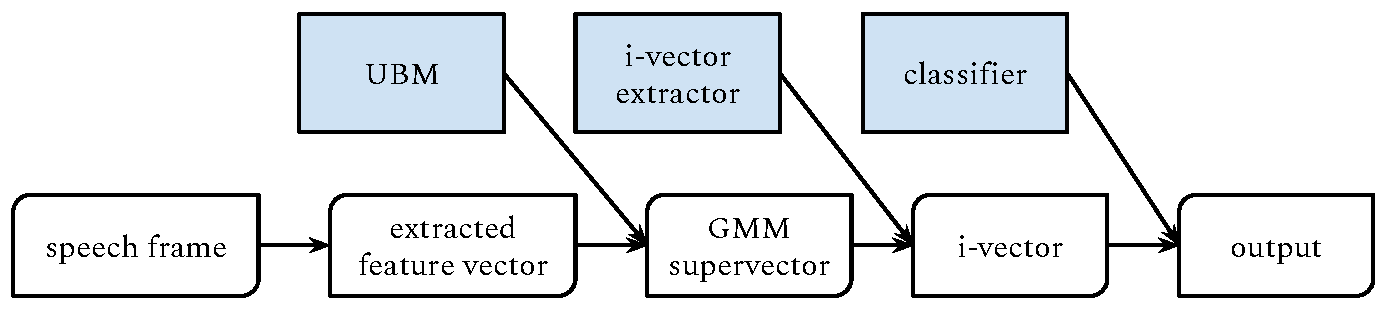
\includegraphics[width=14.5cm]{graphics/i-vectors}
      \vspace*{-1em}
      \caption{Language identification using a typical i-vector system.}
      \label{fig:i-vectors}
    \end{figure}

    The main components of a typical i-vector system, together with their use for prediction, are shown in \autoref{fig:i-vectors}. The universal background model (UBM) is a Gaussian mixture model (GMM) consisting of a large number (e.g. 2048) multivariate mixture components. The UBM is trained using the Expectation-Maximisation algorithm to model the observation space of frame-level feature vectors $\mathbf{x}$ computed from all training utterances (typically 39-dimensional vector using the MFCC features, see \autoref{sec:acoustic-feats}). Given the trained UBM, an utterance $X$ can be represented by a language- and channel-specific GMM supervector $M$ as:
    \begin{equation}
      \label{eq:supervector}
      M_X = m + Tw_X
    \end{equation}
    Here, $m$ is the language- and channel-independent GMM supervector of the UBM (consisting of the stacked means of all mixture components). $T$ is the \textit{total variability matrix} -- also called the i-vector extractor, and $w_x$ is the \textit{identity vector} (i-vector) of sample $X$. The total variability matrix $T$ is "a matrix of bases spanning the subspace covering the important [language and channel] variability in the supervector space" (\citeauthor[p.862]{Martinez_et_al_2011}). Effectively, $T$ projects between the high-dimensional GMM supervector space and the low-dimensional \textit{total variability subspace} (also called the \textit{i-vector space}). The i-vector $w_x$ is then a low-dimensional set of factors projecting the supervector onto the total variability subspace base vectors. The i-vector extractor $T$ is trained again using Expectation-Maximisation (for details see \citet[p. 100]{ivector_tutorial}). Without providing too much detail, I highlight the aspect that is most relevant to my work: training $T$ is based on calculating and further combining the 0\textsuperscript{th}, 1\textsuperscript{st} and 2\textsuperscript{nd} order statistics which are computed by \textit{summing over the frames} of an utterance.

    Once the i-vector extractor has been trained, any utterance can be represented by its i-vector. This enables training a relatively simple and fast classifier operating over the low-dimensional i-vectors. Different classifiers have been successfully used with the i-vector back end; for example, \citeauthor{Martinez_et_al_2011} initially tried using these, all achieving roughly equal performance:
    \begin{enumerate}
      \item {a linear generative model -- modelling the i-vectors of each language by a Gaussian, with a shared full covariance matrix across all language-modelling Gaussians}
      \item {a linear Support Vector Machine computing scores for all languages by doing binary classification in the one-versus-all fashion}
      \item {a two-class logistic regression also doing one-versus-all classification.}
    \end{enumerate}

    At test time, a sequence of feature vectors for utterance $X$ is projected using the UBM into the high-dimensional \textit{supervector space}, producing $M_X$. Then, $T$ is used to extract the utterance-level i-vector, which is processed by the classifier.

    Despite producing utterance-level scores, I describe the i-vector pipeline as shallow because it aggregates frame-level information over time very early (when projecting $X$ into the supervector space), effectively treating an utterance as a bag of frames and disregarding any temporal patterns spanning over multiple frames.
  }

  \section{Less shallow approach: d-vectors}{
    \label{sec:d-vectors}
    % in short: creating utterance-level representations by extracting frame-level information and averaging over frames
    % main difference compared to i-vectors: looking at sequences, i.e. taking each frame's surrounding context into account (this was done by both Variani and Tkachenko)
    % nothing changes about the classifiers, just a different way of producing vectors
    Introduced for speaker verification by \citet{Variani_et_al_2014} and later adapted and applied to language identification by \citet{dvectors_lid}, this approach uses neural networks to extract frame-level information, which is then aggregated across frames to produce utterance- or language-level vectors. Importantly, nothing changes about the final classification stage itself: It is the differences in producing the vector representations what makes i-vectors, d-vectors and x-vectors differ from each other.
    

    % context aggregation done using standard DNN but Tkachenko used TDNN, more familiar from ASR acoustic models and better suited for processing sequences (translation-invariant)
    The biggest change introduced in d-vector systems compared to i-vectors is the notion of frame-level processing while considering each frame's temporal context, i.e. the sequence of a few preceding and following frames. While \citeauthor{Variani_et_al_2014} achieve this by simply feeding the feature vectors of the neighbouring frames together with the frame of interest into a standard deep neural network, \citeauthor{dvectors_lid} use a more suited architecture commonly used for processing temporal sequences in automatic speech recognition: the \textit{time-delay neural network} (TDNN).

    % describing TDNN: like 1D CNN. often made sparse. aggregates information along the time axis
    % TO-DO: Advantages of TDNN over a fully connected DNN?
    % TO-DO: Mention where was TDNN first introduced?
    \begin{figure}[h!]
      \centering
      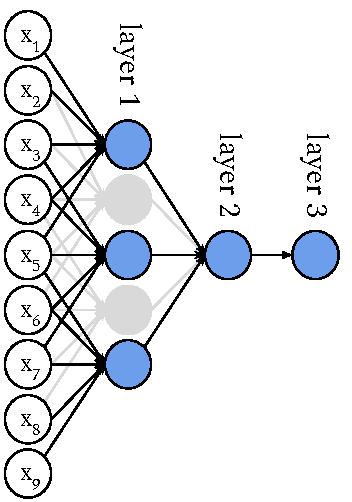
\includegraphics[height=6cm]{graphics/tdnn-generic}
      \caption{Example of a time-delay neural network.}
      \label{fig:tdnn-generic}
    \end{figure}
    A TDNN works like a convolutional neural network (CNN) with 1-dimensional convolutions: only along the time axis, as opposed to the more common 2-dimensional convolutions in image CNNs. \autoref{fig:tdnn-generic} shows a TDNN with three layers which processes information over 9-frame contexts. Note that each blue circle from any layer corresponds to the layer itself (a collection of neurons, i.e. \textit{convolutional kernels}), and all blue circles drawn above each other as corresponding to a particular layer are in fact just one circle -- the layer itself -- sliding over multiple inputs. For example, the convolutional kernels from layer 1 are first applied to feature vectors $\mathbf{x_1}$-$\mathbf{x_5}$, then to vectors $\mathbf{x_3}$-$\mathbf{x_7}$ and then to $\mathbf{x_5}$-$\mathbf{x_9}$. Notice how the network is made more sparse by using \textit{subsampling}, i.e. not using the connections drawn in light grey. A concise and commonly used description of the sketched architecture is shown in \autoref{tab:tdnn-generic} (notice the difference between the interval and set notation); "layer context" meant relative to the preceding layer.
    \begin{table}[h!tb]
      \centering
      \begin{sc}
        \begin{tabular}{l|cc}
                      & Layer context      & Total context \\
          \hline
          layer 1     & $[t-2,\ t+2]$      & 5 \\
          layer 2     & $\{t-2,\ t,\ t+2\}$& 9 \\
          layer 3     & $\{t\}$            & 9 \\
        \end{tabular}
      \end{sc}
      \caption{Example of architecture description of a TDNN (corresponds to \autoref{fig:tdnn-generic}).}
      \label{tab:tdnn-generic}
    \end{table}

    % trained by doing frame-level classification. then the softmax layer ignored and getting activations from the last hidden layer. embeddings! also, GMM supervectors are some kind of embeddings as well ;-)
    In a d-vector system, a TDNN is trained to do direct frame-wise language identification; for this purpose, an additional softmax layer can be added to produce classification outputs. Often, between the convolutional layers and the output layer the architecture contains a few fully connected layers. After training, the classification layer is disregarded and a frame is instead represented by the activation values from the last hidden layer. The TDNN thus serves as a feature extractor, and the representations produced are referred to as \textit{embeddings}.
    % averaging to get utterance-level or language-level vectors.  which after extracting information from frames with contexts, average
    A d-vector representing an entire utterance is then simply the average of the embeddings of all frames from the given utterance.
    
    % even though information is simply averaged across frames, d-vectors made a step beyond bag of frames: temporal features are being extracted, in the case of Tkachenko +-10 (21-frame window), Variani did -30 +10 (41-frame window)
    Despite the naive averaging, utterances are no longer treated merely as bags of frames because each embeddings contains features extracted over short temporal window: 21-frame windows in the case of \citeauthor{dvectors_lid} and 41-frame windows used by \citeauthor{Variani_et_al_2014}, making d-vectors less shallow than i-vectors.
  }

  % TO-DO: justify the use of 'deep'
  \section{Deep utterance-level approach: x-vectors}{
    \label{sec:x-vectors}
    % natural extension to d-vectors: computing not just average but also standard deviation.
    The x-vector approach, introduced last year by the John Hopkins University team first for speaker verification \citep{Snyder_et_al_2018b} and subsequently for language identification \citep{Snyder_et_al_2018}, can be viewed as an extension to d-vectors, producing utterance-level embeddings even for variable-length speech segments. The architecture consists of (see also \autoref{fig:x-vectors-hl}):
    \begin{enumerate}
      \item {the context-aggregating TDNN layers operating at frame level (with the final context window of $\pm$7 frames),}
      \item {a \textit{statistics pooling layer} which computes the mean and the standard deviation over all frames, effectively changing a variable-length sequence of frame-level activations into a fix-length vector, and}
      \item {an utterance-level part consisting of 2 fully connected bottleneck layers which extract more sophisticated features and compress the information into a lower-dimensional space, and an additional softmax output layer.}
    \end{enumerate}
    
    \begin{figure}[h!]
      \centering
      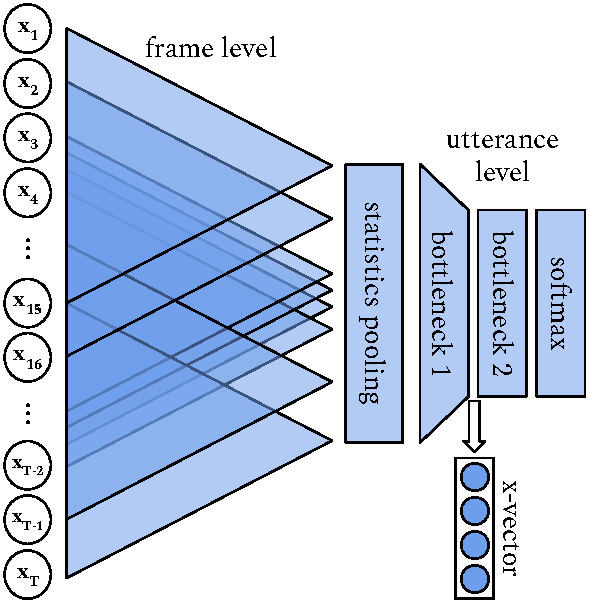
\includegraphics[height=8cm]{graphics/x-vectors-hl}
      \caption{A high-level sketch of the x-vector TDNN from \citeauthor{Snyder_et_al_2018}.}
      \label{fig:x-vectors-hl}
    \end{figure}
    % bottleneck layers to extract _small_ enbeddings
    % biggest difference: TDNN trained to do utterance-level classification (likely to improve the quality of embeddings)
    After the TDNN has been trained, embeddings extracted as the activations of the first bottleneck layer -- named x-vectors -- are then utterance-level representations and can be used directly as input for a final classifier. The biggest difference compared to the d-vector neural networks discussed in \autoref{sec:d-vectors} is that the x-vector TDNN is trained to do not frame-level, but utterance-level classification. The utterance-level statistics (mean and standard deviation) are computed \textit{as part of the network} and are further processed by the additional fully connected layers with non-linear activation functions. These bottleneck layers also make it possible to preserve a higher number of useful features after the statistics-pooling layer: By enabling the last frame-level layer to inflate the representations to 1500-D. The bottleneck layers then learn a transform back to the 512-dimensional space (high-dimensional vectors would be inconvenient for the final classifier) while extracting from the aggregated statistics the features most useful for utterance-level classification (not just for frame-level decisions).

    \begin{table}[h!tb]
      \centering
      \begin{sc}
        \begin{tabular}{cl|ccc}
                      && Layer context      & \thead{Total \\ context} & Number of units \\
          \hline
          \multirow{5}{*}{\rotatebox[origin=c]{90}{frame level\ }}
          &layer 1     & $[t-2,\ t+2]$      & 5             & 512 \\
          &layer 2     & $\{t-2,\ t,\ t+2\}$& 9             & 512 \\
          &layer 3     & $\{t-3,\ t,\ t+3\}$& 15            & 512 \\
          &layer 4     & $\{t\}$            & 15            & 512 \\
          \belowspace
          &layer 5     & $\{t\}$            & 15            & 1500 \\
          \hline
          \multicolumn{2}{c|}{\makecell{statistics pooling \\ layer}} 
                       & $[1,T]$            & utterance     & \makecell{3000-dimensional\\ output} \\
          \hline
          \abovespace
          \multirow{3}{*}{\rotatebox[origin=c]{90}{\shortstack[l]{utter.\\level}}}
          & bottleneck 1& N/A               & utterance     & 512 \\
          & bottleneck 2& N/A               & utterance     & 512 \\
          & softmax     & N/A               & utterance     & \makecell{L-dimensional \\ output} \\
        \end{tabular}
      \end{sc}
      \caption{Description of the x-vector TDNN from \citeauthor{Snyder_et_al_2018} and used in this work. $T$~is the number of frames in a given utterance. Table adapted from \citet[p. 106]{Snyder_et_al_2018}.}
      \label{tab:x-vectors}
    \end{table}

    % trained architecture can be used directly as an end-to-end LID classifier, but found to perform better when x-vectors are extracted and fed into separate classifier. also, adding new languages is possible with classifier and has been shown to perform well even when the TDNN didn't see the language during training
    Because of being an utterance-level classifier, the x-vector TDNN can be used directly as an end-to-end system, although \citeauthor{Snyder_et_al_2018} found that extracting x-vectors and training a separate classifier to classify them yielded lightly better results. Perhaps an even stronger argument in favour of the two-stage process is that, by using an external light-weight classifier, one can easily change the set of supported languages without having to expensively re-train the TDNN. \citeauthor{Snyder_et_al_2018} showed that simply re-training the classifier is enough to gain very good results for languages the TDNN has not observed during training (although the results are indeed worse than those for observed languages).

    % outperforming various optimized variations of i-vectors
    % TO-DO: Define somewhere the metric used to compare the systems and provide concrete numbers?
    The x-vector system consistently beat several state-of-the-art i-vector architectures, which is a particularly interesting finding because i-vector systems have for long been dominant despite the nowadays so "fashionable" and successful deep learning approaches. Even so, the 2-stage x-vector system using a simple classifier still dominates the end-to-end neural network alternative.
  }

  \section{Features used in language identification}{
    \label{sec:features}
    % ASR being the main speech processing area and the powerhorse of research; to an extent, LID systems are motivated by ASR systems which need to know the language first
    Historically, automatic speech recognition (ASR) has been the most important area of speech processing and it has driven forward other areas including language and speaker recognition. In particular, LID systems still exist mostly as part of ASR systems where the language of speech needs to be identified before attempting to transcribe the speech.
    % Hence, most feature engineering has been done with the aim of extracting information useful for ASR -- the speaker- and language-independent information on the phones produced by the vocal tract. These are called acoustic features.
    Hence, data preprocessing and input feature types for LID systems often come from the ASR area. In particular, the feature extraction processes follow the ASR objectives: To extract the language- and speaker-\textit{independent} information important for discriminating between different phonemes produced by a speaker's vocal tract. The feature types devised for this aim are termed \textit{acoustic features}.
    % Acoustic feats can also be described in terms of the information they disregard or do not explicitly capture: information which is language- and speaker-specific -- intonation, stress, pitch range, tone, and others, collectively referred to as prosodic information.
    However, these features can also be characterised by the information they disregard or at least to not capture explicitly: the language- and/or speaker-\textit{dependent} information: intonation, stress, pitch range, tone, and others, collectively referred to as \textit{prosodic information}.
    
    % Since this work focuses on using prosodic information to improve LID, it is useful to understand both acoustic and prosodic features, how they differ and how prosody can be utilised by systems that process frame sequences rather than individual frames.
    As this work focuses on exploiting prosodic information to improve LID, it is desirable to understand both acoustic and prosodic features: how they differ, why is prosody useful and how can prosodic information be modelled in systems that process frame sequences rather than isolated speech frames.

    % TO-DO: Mention that acoustic are more accent-independent while prosodic may be misleading e.g. for non-native speakers.
    
    \subsection{Acoustic features}{
      \label{sec:acoustic-feats}
      % Most common acoustic feats: MFCCs. Their aim is literally to describe the shape of the vocal tract (which maps to the shape of the spectral envelope, which maps to the phone produced).
      The most commonly used acoustic feature type are the Mel-frequency cepstral coefficients (MFCCs). These are coefficients that aim to characterise the shape of the vocal tract, which corresponds to characterising the spectral envelope of produced sounds or, in a way, to the actual phones produced. Without providing too much technical detail, I remind the reader of the main steps in computing MFCCs in \autoref{fig:mfcc} (for details, see for example Chapter 10 of \citet{Holmes_and_Holmes}).
      % Image of MFCC pipeline with high-level descriptions of single steps.
      % - windowing: extracting short temporal frames from the waveform
      % - extracting enery level (loudness) from each frame
      % - discrete fourier transform: extracting spectral information from a single frame (transform from time domain into frequency domain)
      % - mel filterbank: quantifying the energy levels present in discrete, overlapping frequency bands (spaced unevenly to reflect the human perceptual scale), smoothing out pitch information
      % - logarithm: accounting for human non-linear perception of loudness
      % - inverse DFT: extracting coefficients characterising the shape of the spectral envelope
      \begin{figure}[h!]
        \centering
        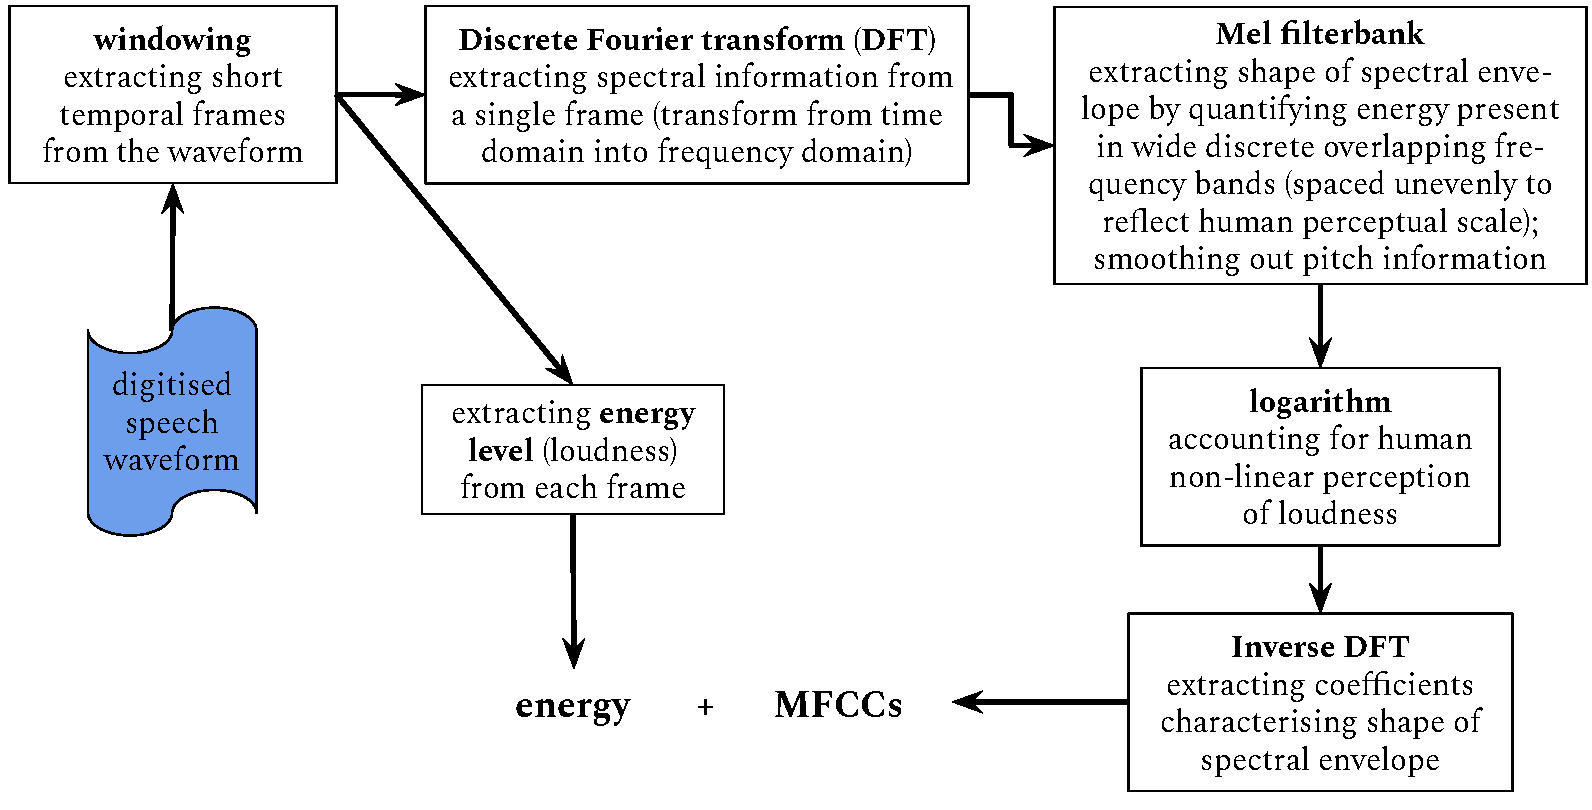
\includegraphics[width=\textwidth]{graphics/mfcc}
        \vspace*{-1em}
        \caption{Main steps in computing the MFCC features including energy. Adapted from \citet[p. 10]{ASR_L2}.}
        \label{fig:mfcc}
      \end{figure}
      % Note that recently, mel filterbanks have been used as well, because neural networks can deal well with correlated features, and doing one less feature processing step is attractive (with each step, some information is lost).

      % To explicitly capture local temporal trends, delta and delta-delta terms are often computed and added to MFCCs or mel filterbanks
      To capture local temporal trends going beyond the single frame level, computed features such as MFCCs are often augmented with frame-specific \textit{dynamic} features -- \textit{delta cepstra} (also just \textit{deltas} or $\Delta$) and double deltas ($\Delta\Delta$). These are simple approximations of the first and second derivatives of the original acoustic feature, and are computed for frame $t$ like this ($\mathbf{x}_t$ is the MFCC feature vector):
      \begin{equation}
        \label{eq:dynamic-feats}
        \Delta(t) = \mathbf{x}_{t+1} - \mathbf{x}_{t-1},\ \ \ \ \Delta\Delta(t) = \Delta(t+1) - \Delta(t-1)
      \end{equation}
      using the context of~$\pm$2~frames. Such dynamic features are justified especially in systems which apply the bag-of-frames approach, not extracting temporal trends (such as the standard i-vector architectures).

      % To capture temporal trends over longer contexts, MFCCs are often turned into SDCs.
      For modelling even longer-range trends specifically in the LID task, \citet{Torres-Carrasquillo_et_al_2002} used an extension of simple deltas called the \textit{shifted delta cepstra} (SDC) features -- essentially, deltas computed at multiple points and stacked together. They can then be used as a new feature vector, or concatenated with the original MFCC vector. SDCs can be configured by setting their 4 parameters: $N$, $d$, $p$, $k$ corresponding to a $N$-$d$-$p$-$k$, a typical one being 7-1-3-7. $N$ refers to the number of first cepstral coefficients taken into account (not necessarily the full MFCC vector), $p$ denotes the distance between consecutive points at which deltas are computed, $d$ determines the size of the window for computing deltas ($d=1$ corresponds to \autoref{eq:dynamic-feats}) and $k$ is the number of points at which to compute deltas. The SDC terms for frame $t$ and to be stacked together are then:
      \begin{equation}
        \label{eq:sdc-feats}
        \Delta_{SDC}(t+ip) = \mathbf{x}_{t+ip+d} - \mathbf{x}_{t+ip-d} \quad\quad \forall i \in \{0, ..., k-1\}
      \end{equation}
      % SDC used by \cite{Ferrer_et_al_2016} and \cite{Sarma_et_al_2018} (7D MFCC + 7-1-3-7 SDCs = 56D) and by \cite{Torres-Carrasquillo_et_al_2002} (10-1-3-3)
      As with standard deltas, capturing long-range trends with SDCs can certainly be beneficial for i-vector systems. \cite{Ferrer_et_al_2016} used an i-vector system with SDC features as the state-of-the-art baseline system for their novel experiments. Additionally -- following the successful application of SDCs by \citeauthor{Torres-Carrasquillo_et_al_2002} in a pre-i-vector system, \cite{Sarma_et_al_2018} report slightly better results with SDCs compared to using high-resolution MFCCs when training an i-vector architecture with a deep neural network UBM. Still, the usefulness of SDCs is not so clear in architectures inherently able to extract temporal trends.

      % Advantage of acoustic features for LID: where LID is part of ASR, acoustic feats are available anyway, hence there's no need to compute different feats just for the LID part.
      Compared to the prosodic features described next, the discussed classic acoustic features have one clear advantage where the LID system is part of a bigger ASR pipelines: The two systems can share the same feature vectors without the need to compute additional features solely for the purpose of language identification.

      % MFCCs also used inderectly to train ASR DNNs which then provide bottle-neck features which give very promising results in both LID and SID
    }

    % LEL2D lecture on tone: https://www.learn.ed.ac.uk/bbcswebdav/pid-2255587-dt-content-rid-4289141_1/courses/LASC080202016-7SV1SEM2/week05.02.html
      % A language with tone is one in which an indication of pitch enters into the lexical realization of at least some morphemes (Hyman 2006) Hyman, Larry M. 2006. Word-prosodic typology. Phonology 23(2). 225–257.
      % A language is a ‘tone language’ if the pitch of the word can change the meaning of the word. Not just its nuances, but its core meaning. (Yip 2002) Yip, Moira. 2002. Tone. Cambridge: Cambridge University Press.
    \subsection{Prosodic features}{
      \label{sec:prosodic-feats}
      % OLD MATERIAL TO BE RE-USED
        % compared to well-established acoustic feats, there is no good definition of prosodic feats and they are not commonly used
        % for the purposes of this work, I narrow down the prosodic variables to four: intonation+tone, stress and rhythm. TO-DO: these should be the main ones, cite some paper?
        
        % both intonation and tone are perceived qualities, typically associated with the variation of the physical quality called pitch, i.e. the fundamental frequency of vibration of the vocal folds (also denoted as F_0). 
        % while the term 'tone' is used where pitch variation is contrastive (i.e. changes to it discriminate between different words) in the so-called tonal languages (such as Chinese, Vietnamese, Thai), intonation denotes the non-contrastive pitch variation mostly associated with speaker's emotions, dialect, social background, speaking style, and other factors (see, for example, this study by \citet{Grabe_2004} on the intonation differences across British English dialects).
        % note: some recent results show what other physical variables can influence perceived intonation, but these are disregarded for now. TO-DO: find those works?
        % \citet{Lin_et_al_2005} do LID just from the segmented pitch contour, each short pitch segment (around 100-200ms) parametrised by a few Legendre polynomials -- not too much success
        % \citet{Metze_et_al_2013} show improvements in ASR on tonal (and partly on non-tonal) languages when including F0 variation feats.
        % \citet{Song_et_al_2013} achieve LID improvements when using bottleneck features trained on MFCC+pitch vectors
        % One disadvantage of pitch contours: F0 is undefined for unvoiced sounds, hence the computed pitch contour is not continuous.
        % \cite{Ghahremani_et_al_2014} show ASR improvements with a pitch-tracking algorithm that calculates pitch even for unvoiced frames, creating continuous pitch contours. to the best of my knowledge, this feature type hasn't yet beet applied in an LID task.

        % stress (also termed accent) is an unstable term, generally referring to relative emphasis on certain syllables or words and realised as a variation in loudness (dynamic accent), pitch (pitch accent) or length (quantitative accent).
        % ASR models dynamic and quantitative accent implicitly under certain conditions when using acoustic feats. but I isolate 

        % in this work, I contrain myself to using two feature types for modelling prosody: 
        % - continuous pitch contours extracted using the KaldiPitch algorithm (introduced by \cite{Ghahremani_et_al_2014}) - I refer to this as the pitch feature
        % - raw energy capturing the loudness of speech and modelling dynamic stress (at both word and sentence level)
      % END OF OLD MATERIAL

      % NEW MATERIAL
      % 1. short intro into prosody (cite WALS where appropriate)
      % Prosody stands for information other than that about the produced phonemes. Standard elements: intonation/tone, stress, rhythm. As shown below, each of these can be used to differentiate between languages.
      Prosody is about information other than that directly describing the produced phones; the standard elements of prosody are: intonation/tone, stress and rhythm \citep{Prieto_et_al_2018}. As discussed below, importantly, each of these elements can be used to differentiate between languages.
      \begin{itemize}
        % - intonation and tone are perceived qualities, typically associated with the variation of the physical quality called pitch, i.e. the fundamental frequency of vibration of the vocal folds (F0). while the term 'tone' is used where pitch variation is contrastive (i.e. changes to it discriminate between different words) in the so-called tonal languages (such as Chinese, Vietnamese, Thai), intonation denotes the non-contrastive pitch variation mostly associated with speaker's emotions, dialect, social background, speaking style, and other factors (see, for example, this study by \citet{Grabe_2004} on the intonation differences across British English dialects).
        \item {\textit{Intonation} and \textit{tone} are perceived qualities typically associated with the variation of the physical quality called pitch, i.e. the fundamental frequency of vibration of the vocal folds ($F_0$). The term 'tone' is used where pitch variation is contrastive (i.e. changes to it discriminate between different words): in the so-called \textit{tonal languages}, such as Chinese, Vietnamese and Thai. In each of these languages, a small 'alphabet' of distinct tone levels or tone contours (also called \textit{tonemes} \citep{Trask_2004}) can be observed as it conveys meaning. Intonation, on the other hand, denotes the non-contrastive pitch variation mostly associated with the speaker's emotions, language, dialect, social background, speaking style, and other factors (see, for example, the study by \citet{Grabe_2004} on the intonational differences between different British English dialects).}
        % - stress (also termed accent) is an unstable term, generally referring to relative emphasis on certain syllables or words and realised as a variation in loudness (dynamic accent), pitch (pitch accent) or vowel length (quantitative accent). Specific lexical (syllable-level) stress patterns or rules are often characteristic of a language, e.g. the position of stress is fixed to different positions within word in Czech and Polish (fixed stress), or describable by a set of rules in Arabic (rule-based stress, this needs citation).
        \item {\textit{Stress} (also termed \textit{accent}), despite being a somewhat ambiguous term, generally refers to the relative emphasis on certain syllables within a word or words within a sentence, realised as a variation in loudness (\textit{dynamic accent}), pitch (\textit{pitch accent}) or vowel length (\textit{quantitative accent}). Specific \textit{lexical} (intra-word, i.e syllable-level) stress patterns or rules are often characteristic of a language. For instance, the within-word location of stress is fixed but different for Czech and Polish (\textit{fixed stress}, see \citet{WALS_14}), or describable by a set of rules in Arabic (\textit{rule-based stress}, see \citet{WALS_15}).}
        % - rhythm typically refers to syllable lengths, with the theory of isochrony categorising languages into three types based on their rhythm: syllable-timed, e.g. french or turkish (all syllables have roughly equal durations), mora-timed, e.g. slovak or japanese (all moras have equal durations) and stress-timed languages, e.g. german, arabic (intervals between stressed syllables are of equal durations).
        \item {\textit{Rhythm} refers to regularity in sub-word unit lengths, with the most recognised theory of \textit{isochrony} categorising languages into three types based on their rhythm: \textit{syllable-timed} where all syllables have roughly equal durations (e.g. French or Turkish), \textit{mora-timed} where all moras\footnote{Mora is a basic timing unit; a long syllable having two moras and a short syllable having one mora. See \citet[p. 312]{Crystal_2008} for a broader definition and discussion.} have equal durations (e.g. Slovak or Japanese), and \textit{stress-timed} languages, e.g. German and Arabic (here, the intervals between stressed syllables are of equal durations).}
      \end{itemize}

      % isochrony details
        % syllable-timed: french, spanish, mandarin, turkish
        % mora-timed: japanese, slovak, tamil (https://www.sissa.it/cns/Articles/TBC_048.pdf)
        % stress-timed: thai, german, russian, swedish, portuguese (EU), arabic
        % bulgarian (http://www.personal.reading.ac.uk/~llsroach/phon2/sdjipa.htm), polish (https://www.sissa.it/cns/Articles/TBC_048.pdf): between stress-timed and syllable-timed

      % TO-DO: comment on temporal ranges? 15 frames cover variation across maybe 1-2 syllables. duration of syllable: some 100-200 ms (https://core.ac.uk/download/pdf/84560.pdf)
      % 2. what prosodic aspects acoustic features can capture: rhythm, quantitative stress
      % some of the mentioned prosodic aspects can in fact be captured even when using acoustic features like MFCCs. because prosody surfaces as temporal variation, systems which extract features from frame sequences (such as x-vectors) have the potential to capture it (unlike i-vector systems which apply the bag-of-frames approach). MFCCs can contain information about loudness (in the form of the energy-based C0 cepstral coefficient), which enables capturing dynamic stress. even without using C0, quantitative accent should be possible to capture using acoustic features. regarding rhythm, the temporal trends should be possible to capture for syllable-timed and mora-timed languages, but not necessarily for stress-timed languages (if C0 is not used or if the stress patterns rely heavily on pitch accent which cannot be captured using acoustic features). considering the prosodic aspects that acoustic features alone could theoretically capture, the most important prosodic feature that can be added to the input is pitch: to enable modelling pitch accent, tone, and language-specific intonation.
      Before turning to bespoke alternative features for modelling prosody, it should be noted that some prosodic aspects can be captured by acoustic features like MFCCs. Because prosody surfaces as temporal variation, systems which extract information from frame sequences (such as TDNN-based systems) have the potential to capture it. MFCCs can be (and often are) used together with energy (see \autoref{fig:mfcc}), which enables capturing dynamic accent. Even without using energy as part of MFCCs, the quantitative accent should be possible to capture because durations of vowels are preserved as a result of windowing extracting the frames at evenly spaced points of a speech waveform. Regarding rhythm, the duration regularity (isochrony) should be possible to capture for syllable-timed and mora-timed languages because syllable boundaries occur at phoneme boundaries, which are captured by acoustic features. For stress-timed languages, however, the units with equal durations are marked by stressed syllables, meaning that this regularity may not be fully captured -- in particular if an energy measure is not included in MFCCs, or if the stress is realised as a variation in pitch rather than in loudness. Considering the prosodic aspects that acoustic features alone \textit{could} theoretically capture, I conclude that the most important prosodic feature that can be deemed complementary to acoustic features and added to the input is pitch: to enable modelling pitch accent, tone, and language-specific intonation.


      % 3. what prosodic aspects have been modelled explicitly: intonation/tone/pitch accent (pitch contours)
      % perhaps unsurprisingly, extracting information from pitch for LID has been explored in the past -- although the number of studies very small compared to those using conventional acoustic features. long before i-vectors, \citet{Lin_et_al_2005} attempted LID just from the pitch contour segmented into syllable-like units (around 100-200ms), contour segments parametrised by a few Legendre polynomials. later, \citet{Metze_et_al_2013} show improvements in ASR on tonal (and partly on non-tonal) languages when augmenting MFCCs with F0 variation features. One disadvantage of pitch contours: F0 is not present for unvoiced sounds, hence a pitch contour computed from F0 is not continuous. this issue was addressed by \cite{Ghahremani_et_al_2014} who developed a pitch-tracking algorithm that approximates the pitch contour even for unvoiced frames, making it continuous. they report improved ASR performance mainly on tonal languages. to the best of my knowledge, this feature type hasn't yet beet applied in an LID task.
      Perhaps unsurprisingly, extracting information from pitch for LID has been explored in the past -- although the number of studies is very small compared to those using the conventional acoustic features. Long before i-vectors, \citet{Lin_et_al_2005} attempted to do language identification solely from the pitch contour. This was segmented into syllable-like units (around 100-200ms), each contour segment subsequently represented as the first few coefficients of its approximation by Legendre polynomials. Even though the results were far from those achieved by today's systems, it was demonstrated that LID can be done on pitch information alone. Later, \citet{Martinez_et_al_2012} successfully applied a similar approach to modelling energy and pitch contours within small segments, additionally trying to capture rhythm by providing the duration of voiced speech within the segment as an additional feature. Fusing such prosodic system with an acoustic i-vector system significantly improved the performance. Later, \citet{Metze_et_al_2013} showed improvements in ASR on tonal (and partly on non-tonal) languages when augmenting MFCCs with custom-designed $F_0$ variation features. Nevertheless, one disadvantage of using pitch persisted: The fact that $F_0$ is typically considered to be only present in voiced sounds and undefined for unvoiced ones -- making a pitch contour based on $F_0$ discontinuous. While \citet{Martinez_et_al_2012} effectively ignore this issue by discarding unvoiced frames and thus ending up modelling contours which indeed contain sudden jumps, the problem was addressed in a more elegant way recently by \cite{Ghahremani_et_al_2014}. They developed a pitch-tracking algorithm that approximates pitch values even for unvoiced regions and produces a continuous pitch contour. Adding this feature to MFCCs, the authors report improved ASR performance mainly on tonal languages. To the best of my knowledge, this feature type has not yet been used for language identification.

      % 4. what features I use to explicitly model prosodic aspects: KaldiPitch, raw energy
      % In this work I explore two feature types that explicitly help to capture prosodic information: energy and pitch. I refer to these as the prosodic features.
      In this work, I explore two feature types that explicitly help to capture prosodic information: \textit{energy} and \textit{pitch}. I refer to these as the prosodic features.
      \begin{itemize}
        % By energy I mean the logarithm of the raw energy extracted in the MFCC pipeline right after pre-emphasis and windowing. To isolate the effects of using this prosodic feature, I do not include it in any of the acoustic features used in this work.
        \item {By energy I mean the logarithm\footnote{The use of logarithm is given solely by the Kaldi toolkit I use for feature extraction, although it is by no means an arbitrary design decision: Human perception of loudness is non-linear and logarithm is used also in the standard MFCC computation pipeline (see \autoref{fig:mfcc}).} of the raw energy extracted in the MFCC pipeline right after windowing (as shown in \autoref{fig:mfcc}). To isolate the effects of using this prosodic feature, I do not include it in any of the acoustic features used in this work. However, I do not exclude the 0\textsuperscript{th} cepstral coefficient from MFCCs, even though it bears some loudness-related information; more specifically, it can be considered as "a collection of average energies of each frequency bands in the signal that is being analyzed" \citep{Zheng_and_Zhang_2000}.}
        % By pitch I mean the continuous pitch extracted using the algorithm presented by \citeauthor{Ghahremani_et_al_2014}.
        \item {By pitch I mean the continuous pitch (and features derived from it) extracted using the Kaldi pitch algorithm presented by \citeauthor{Ghahremani_et_al_2014}. Because this feature type is not well known, I elaborate on it in the next section.}
      \end{itemize}
    }
    \subsection{The continuous Kaldi pitch as a prosodic feature}{
      \label{sec:kaldi-pitch}
      Even though the original paper \citep{Ghahremani_et_al_2014} contains a detailed description of the Kaldi pitch algorithm (along with a working implementation as part of the Kaldi ASR toolkit), I provide an additional, more holistic view to give the reader an intuitive understanding of the algorithm and the features it produces (see \autoref{fig:kaldi-pitch}).
      \begin{figure}[h!]
        \centering
        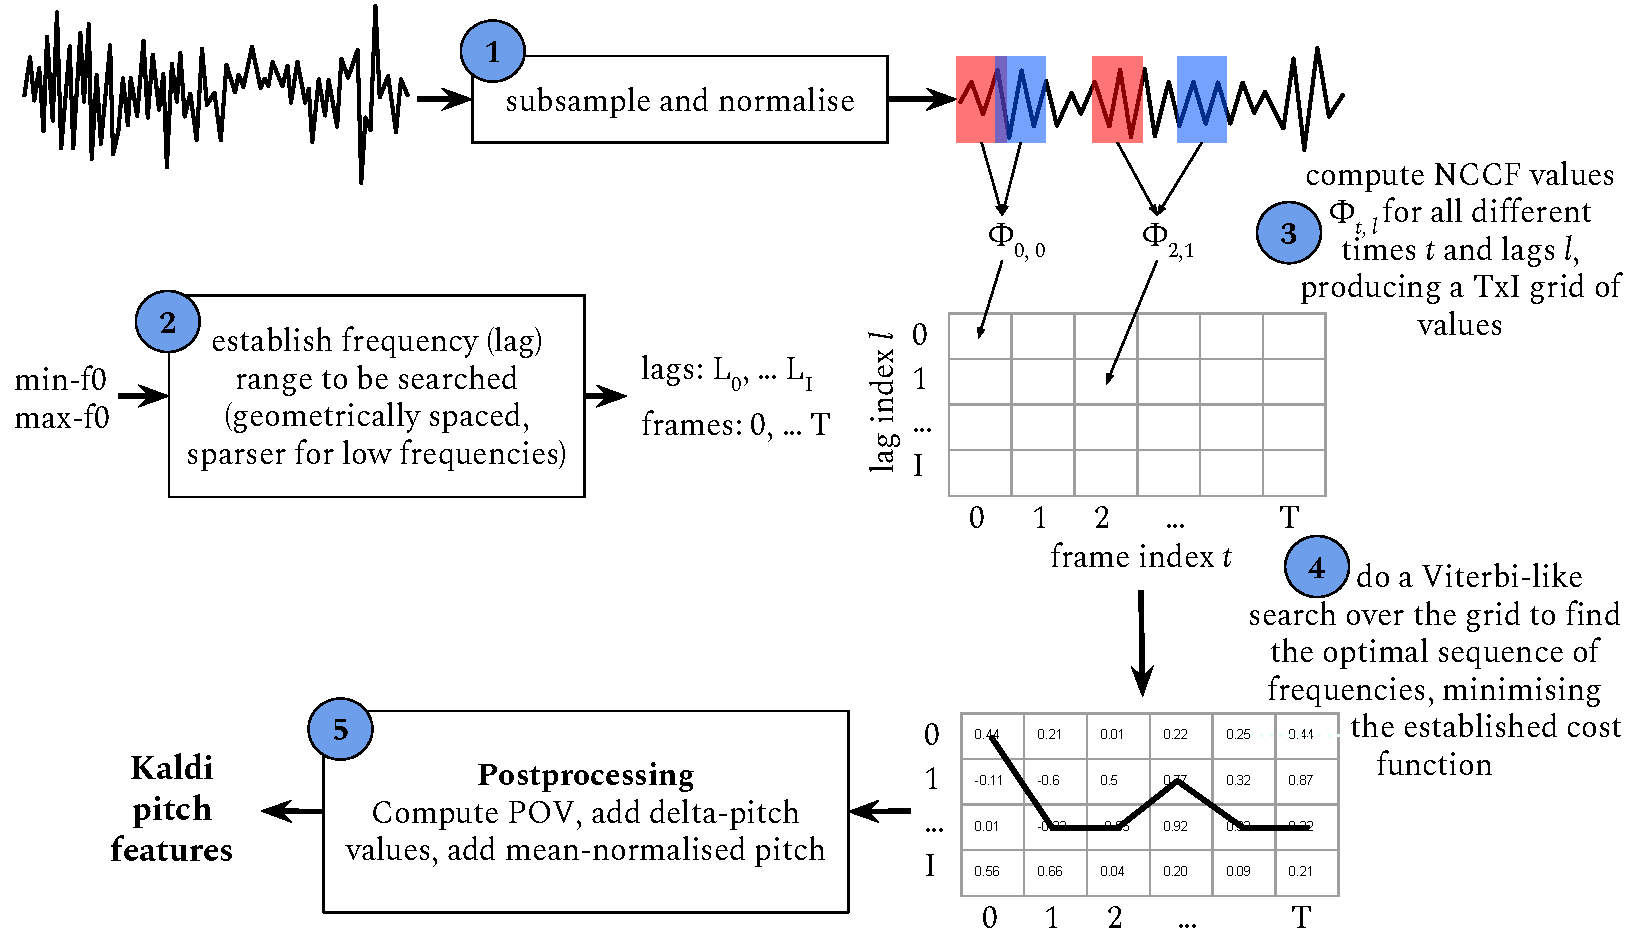
\includegraphics[width=\textwidth]{graphics/kaldi-pitch}
        \vspace*{-1em}
        \caption{The steps of the Kaldi pitch algorithm.}
        \label{fig:kaldi-pitch}
      \end{figure}
      % diagram and formulae describing KaldiPitch.
      % - subsample and normalise (divide by root mean square)
      % - establish frequency range to be searched (geometrically spaced, more sparse for lower frequencies)
      % - compute NCCF for all different time positions and lags, producing a grid of values TxI. the NCCF computation includes the ballast term which makes the values close to zero for very weak normalised cross-correlation values
      % - define cost function for a sequence of frequencies (a pitch contour): penalising low NCCF values, too low frequencies and big frequency jumps
      % - do a Viterbi-based search over the grid to find the optimal sequence of frequencies
      % Postprocessing:
      % on top of the raw pitch, add:
      % - probability of voicing (POV): converting the NCCF values (which have range [-1,1]) to a feature which was empirically found to work well for ASR in multiple languages
      % - normalised pitch: weighted-mean subtraction over windows of 151 frames (+-75), with weights roughly corresponding to log(p(voiced)/p(unvoiced))
      % - delta terms computed over windows of +- 2 frames from the unnormalised pitch
      Perhaps the biggest contribution lies in abandoning the binary decision making about voiced/unvoiced speech, and only calculating pitch for the voiced frames. Instead, soft decisions are made based on the values of the normalised cross-correlation function (NCCF). For two pieces of digitised waveform separated by temporal distance $l$ from each other and represented as vectors $\mathbf{v}_{t, 0}$ and $\mathbf{v}_{t, l}$, the NCCF is computed as follows (adapted from \citeauthor[Eq. 2]{Ghahremani_et_al_2014}):
      \begin{equation}
        \label{eq:nccf}
        \Phi_{t, l} = \frac{\mathbf{v}_{t, 0}^T \mathbf{v}_{t, l}}{\sqrt{(\mathbf{v}_{t, 0}^T \mathbf{v}_{t, 0})(\mathbf{v}_{t, l}^T \mathbf{v}_{t, l})+B}}
      \end{equation}
      where normally $B=0$, but the authors use a non-zero value to push the NCCF values towards 0 where the cross-correlation on its own is very low. By computing NCCF for different spacings $l$  -- called \textit{lags} by the authors, and being effectively the periods of different hypothesised frequencies -- one obtains continuous confidence values about the presence of the corresponding frequencies in the signal for the time position $t$. After computing these for all temporal positions, the algorithm finds the optimal continuous contour by minimising the proposed cost function (see \citeauthor[Eq. 4]{Ghahremani_et_al_2014}), which prefers higher NCCF values and penalises too low frequencies and too big frequency jumps.

      Finally, the algorithm post-processes the raw pitch contour to provide these additional features:
      \begin{enumerate}
        \item {A mean-normalised pitch contour, with the mean computed over 151-frame windows and weighted by a measure roughly corresponding to the log likelihood of a particular frame being voiced (i.e. putting more weight on voiced frames).}
        \item {\textit{Probability of voicing} (POV): A feature which is not a probability, but acts similarly and has been empirically found by the authors to provide improvements in ASR performance.}
        \item {Delta-pitch terms, computed in the same way as the simple deltas in \autoref{eq:dynamic-feats}.}
      \end{enumerate}
      In this work, I work with all four feature types (the raw pitch contour and the three derived feature types) and refer to them collectively as the Kaldi pitch.
    }

    \subsection{Illustrating the prosodic features used in this work}{
      Having familiarised the reader with the two prosodic features I will use (the energy and the Kaldi pitch), I now illustrate them on a realistic example. Because the multi-lingual corpus used for this project does not contain English, I used the freely accessible sample utterance from the CSR-I (WSJ0) Complete corpus\footnote{\url{https://catalog.ldc.upenn.edu/LDC93S6A}}, which has important characteristics such as the recording conditions and the speaking style the same as the corpus I later use (see \autoref{sec:GlobalPhone}).
      \begin{figure}[h!]
        \centering
        \vspace{-1.2em}
        \hspace*{-2.4cm}
        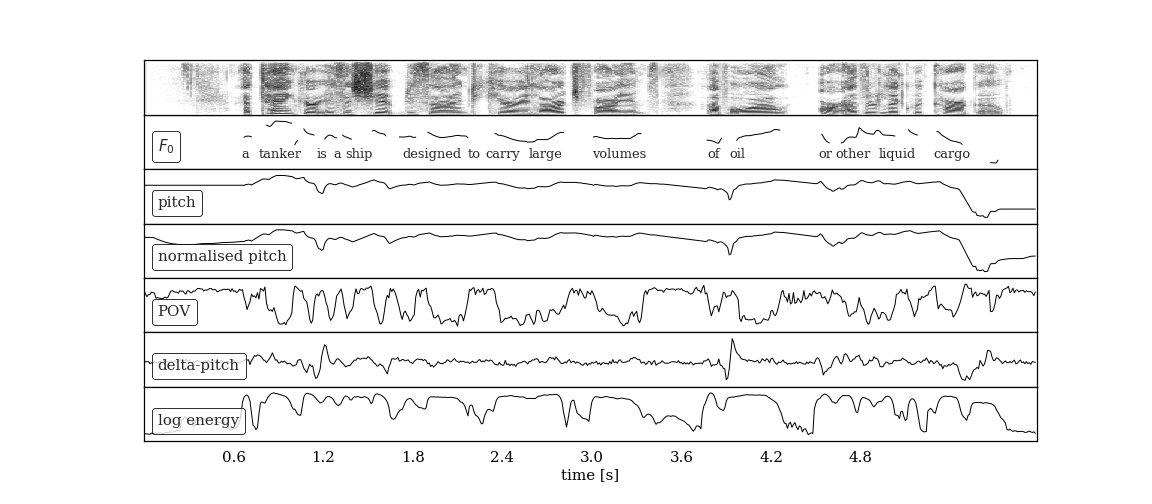
\includegraphics[width=18.7cm]{../img/prosody_sample.png} % TO-DO: Eventually change to PDF (compilation then takes long).
        \vspace*{-3em}
        \caption{The prosodic features I use in this project (together with the spectrogram and the fundamental frequency $F_0$), illustrated on an English utterance. I manually created the time-aligned transcription for better understanding.}
        \label{fig:prosodic-feats}
      \end{figure}
      
      \autoref{fig:prosodic-feats} shows the prosodic features on the English utterance. For clarity and comparison, I added the spectrogram as well as the discontinuous $F_0$ contour -- both generated in Praat \citep{Praat}. As expected, the $F_0$ segments match the Kaldi pitch contour. Notice how the Kaldi pitch does not drop in unvoiced regions, but rather behaves like a smooth bridging between the regions. Also note that the POV values are effectively negated: High values corresponding to the regions where true $F_0$ is absent and low values marking the voiced regions.
    }
  }
}

\chapter{Data -- GlobalPhone}{
  \label{chap:Data}
  % LID often part of ASR, hence it makes sense to train on the same corpora
  Because LID systems are often part of ASR systems, it makes sense to use the same datasets to train both.
  % additionally, NIST has been having the LREs. which are now THE benchmarking datasets for LID. but they only to narrowband telephone speech...
  Additionally, however, the U.S. National Institute of Standards and Technology (NIST) has been organising dedicated Language Recognition Evaluation\footnote{\url{https://www.nist.gov/itl/iad/mig/language-recognition}} (LRE) challenges since 1996, providing multilingual datasets which are today the standard benchmark for evaluating language recognition systems (used also by \citet{Snyder_et_al_2018}). The NIST datasets, however, only focus on narrowband (8kHz) conversational telephone speech and include strong channel variability as a result of the uncontrolled recording environment, which makes it more difficult to analyse any observed effects and attribute them to particular language pair similarities or particular prosodic aspects.
  % I use the relatively small multilingual ASR corpus which is in many aspects different from the NIST data
  In this work, I use a relatively compact ($\sim$400 hours of speech) corpus which is in many aspects different from the NIST datasets.

  \section{Overview of the GlobalPhone corpus}{
    \label{sec:GlobalPhone}    
    % copies the style of the CRS-I corpus: newspaper articles read by native speakers
    % started in 1995, presented in 2002 and 2013 (citations). I use the newest version from 2016 which contains 22 languages.
    The corpus I use is the GlobalPhone multilingual ASR corpus \citep{Schultz_et_al_2013}, more precisely its newest version -- updated in 2016 and covering 22 languages from around the world (see \autoref{fig:GlobalPhone-map}): Arabic (AR), Bulgarian (BG), Chinese-Mandarin (CH), Chinese-Shanghai (WU), Croatian (CR), Czech (CZ), French (FR), German (GE), Hausa (HA), Japanese (JA), Korean (KO), Brazilian Portuguese (PO), Polish, (PL), Russian, (RU), Spanish, (SP), Swahili (SWA), Swedish (SW), Tamil (TA), Thai (TH), Turkish (TU), Ukrainian (UA), and Vietnamese (VN). The corpus follows the style established for English by the Wall Street Journal-based corpora \citep{Paul_Baker_1992} such as the CSR-I (WSJ0) Complete corpus\footnote{\url{https://catalog.ldc.upenn.edu/LDC93S6A}}. It consists of newspaper articles read by native speakers (around 100 speakers per language, each speaker producing about 20 minutes of audio by reading 3-5 articles), recorded as wideband (16kHz) audio in a controlled environment, using a close-talking microphone (in the case of GlobalPhone the Sennheiser microphone HD-440-6).

    \begin{figure}[h!]
      \centering
      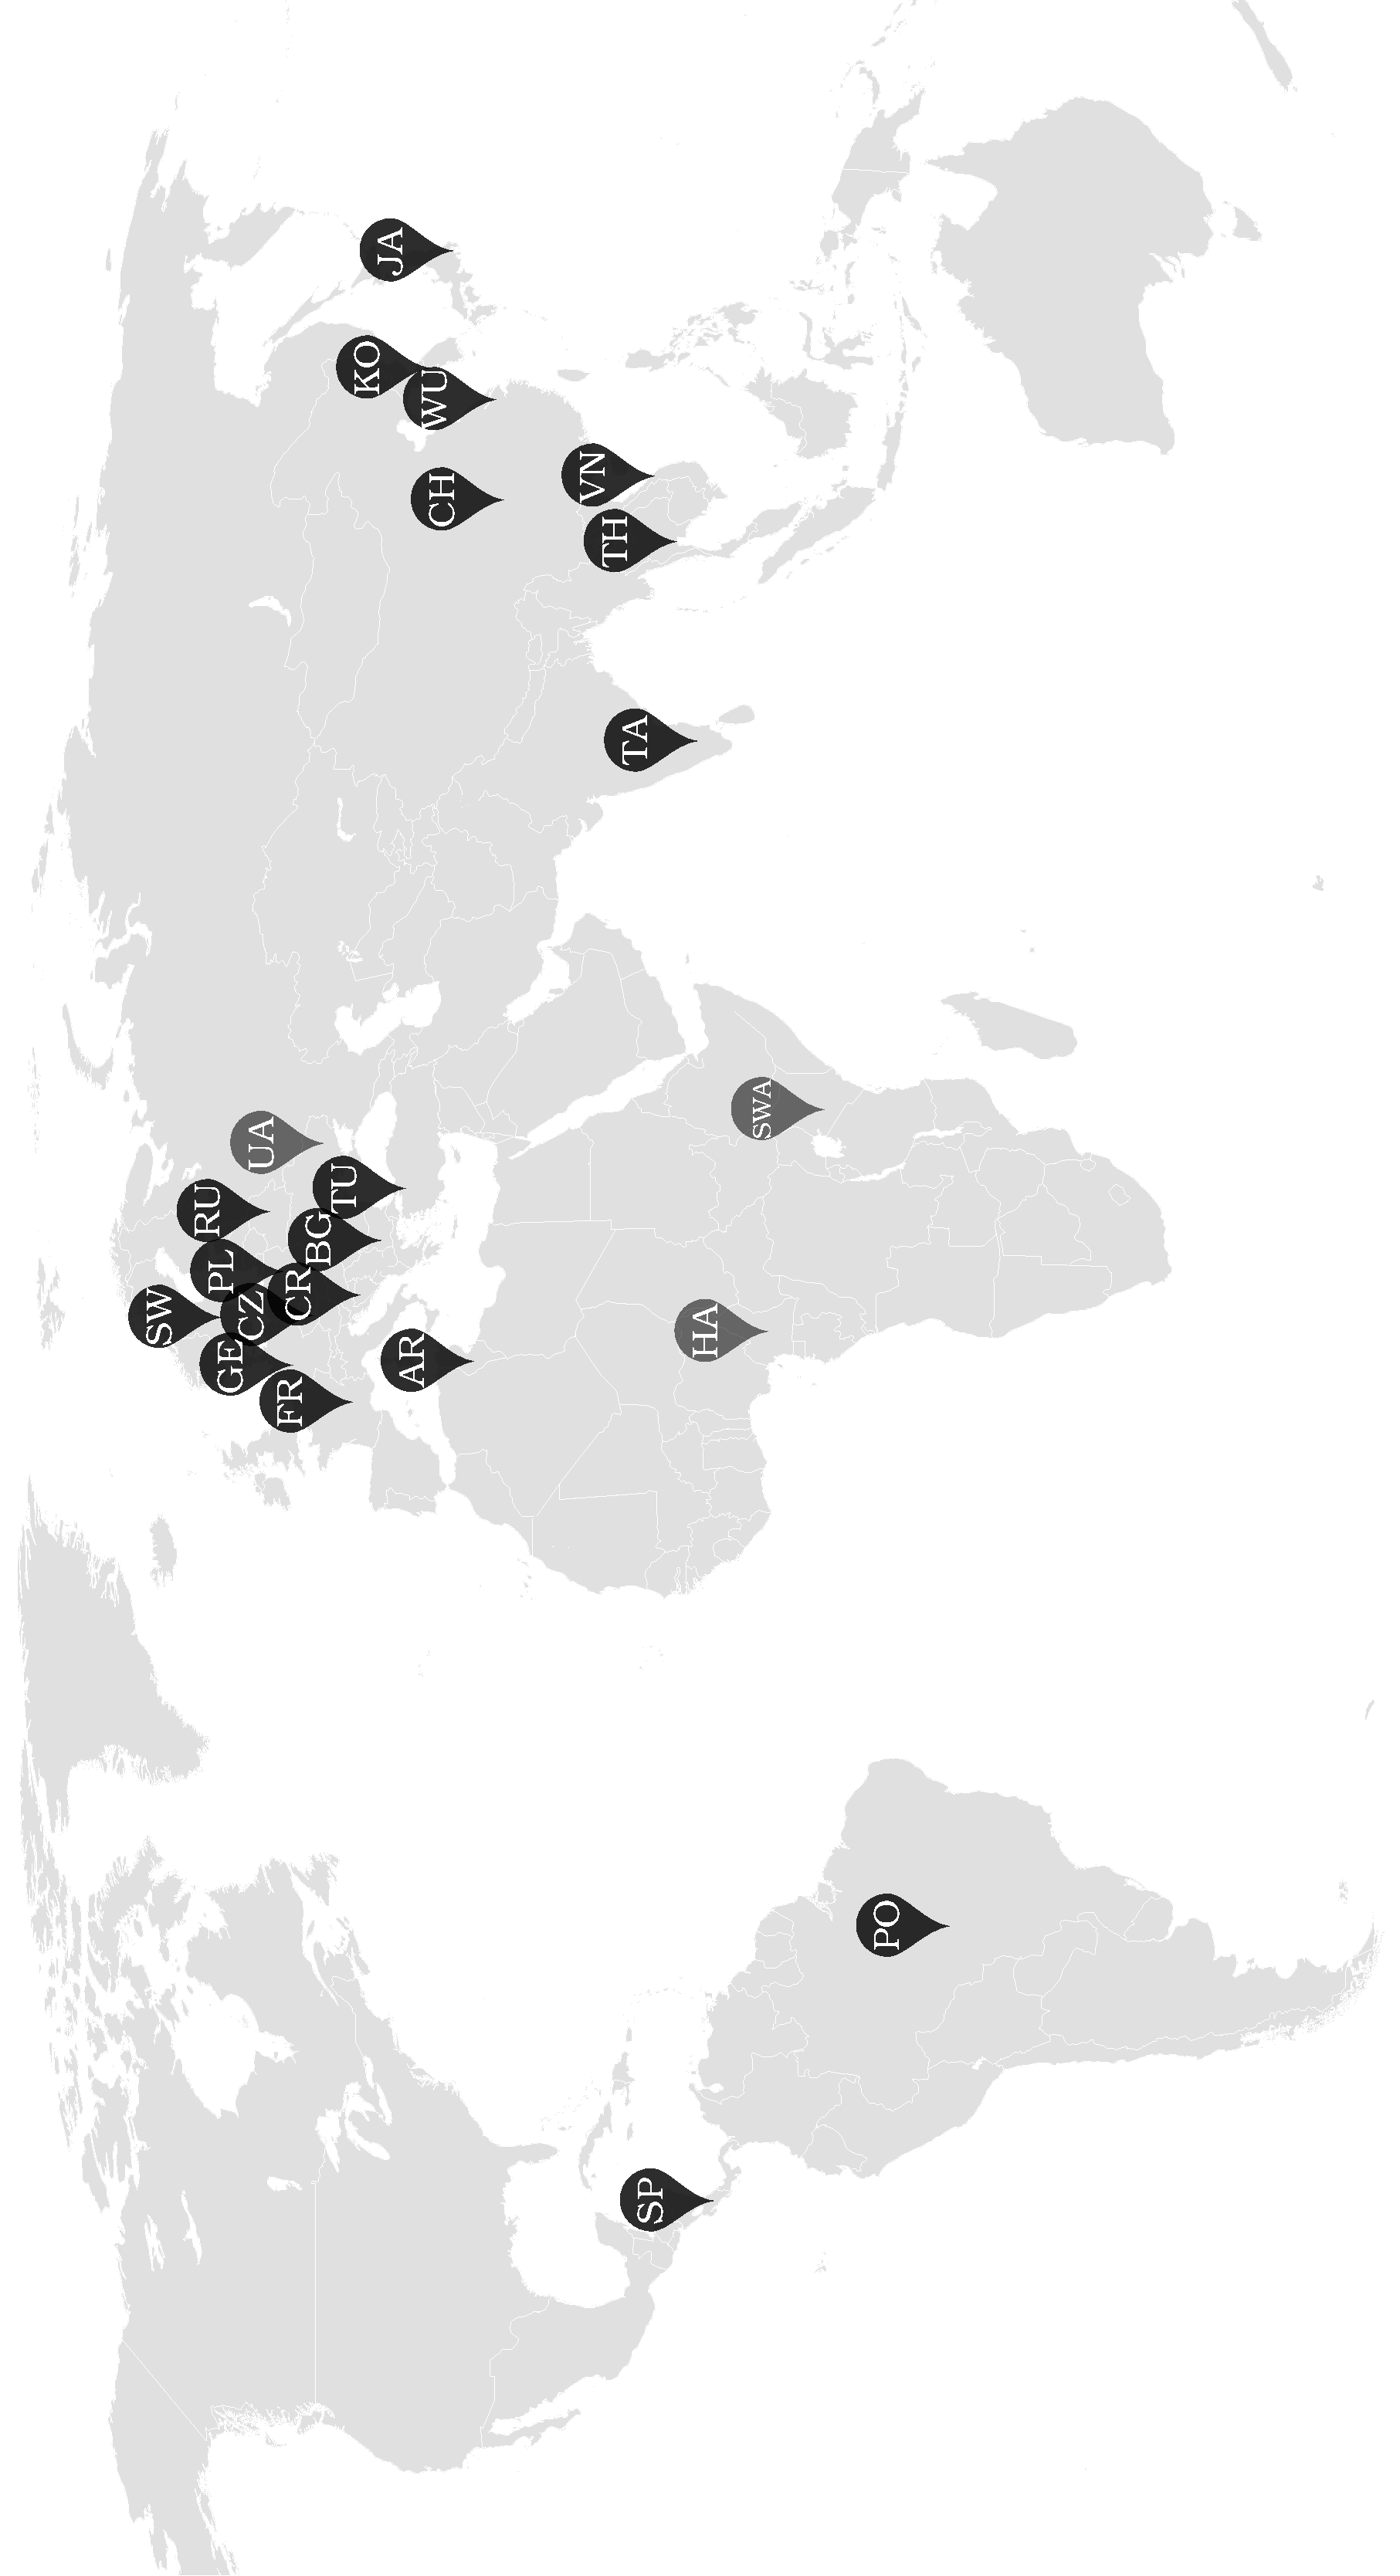
\includegraphics[width=7.7cm, angle=270]{graphics/GlobalPhone-map.pdf}
      \vspace*{-1em}
      \caption{Languages of GlobalPhone as shown roughly at the location where they were recorded. Greyed out are Hausa, Swahili and Ukrainian -- the three languages I did not use in this work due to corrupt data (see \autoref{sec:invalid-data}). Also notice that Russian was, in fact, recorded in Belarus, and Spanish in Costa Rica.}
      \label{fig:GlobalPhone-map}
    \end{figure}
    
    % wideband, controlled clean recording conditions -- good for reasoning! (don't need to worry about results being affected by channel differences)
    The controlled environment, speaking style and nature of the texts (all are major newspaper articles) make the data better suited for analysing effects of, for example, prosodic features: Any observed trends can be more reliably attributed to my controlled independent variables (such as the feature type) or to the known language differences.
    % Plus (compared to NIST): rich vocabulary (newspaper articles).
    Another advantage of the GlobalPhone corpus is the rich vocabulary (compare with short telephone conversations in the NIST corpora).
    Finally, from a linguistic view, the corpus covers a wide range of language families and prosody-based categories, while also providing an interesting sample of related languages in the form of 5 Slavic languages (which the author -- as a native speaker of Slovak -- can relate to): Bulgarian, Czech, Croatian, Russian, and Ukrainian.

    % Minus: no spontaneous speech! And no channel variation! (for LID on YT videos)
    Unfortunately, the corpus does not cover spontaneous speech (which -- as known in ASR -- is much more challenging than read text). The extremely low channel variability is also a tight constraint and it is possible that, even if prosodic features improve LID performance on this dataset, the results will not necessarily generalise well to more realistic scenarios with greater channel variability and noise.    
  }

  \section{Data partitioning}{
    \label{sec:partitioning}
    GlobalPhone ships with a partitioning of each language's data into training, evaluation and testing (in GlobalPhone documentation referred to as training, development and evaluation, respectively) sets, with the sizes of the 3 partitions being roughly 80\%, 10\%, 10\%, respectively. However, for the purposes of the x-vector architecture, a 4-way partitioning is required:
    \begin{enumerate}
      \item{training set -- for training the x-vector TDNN,}
      \item{enrollment set -- for training the x-vector classifier,}
      \item{evaluation set -- for tuning the hyperparameters of both the TDNN and the classifier,}
      \item{testing set -- for final end-to-end evaluation on unseen data.}
    \end{enumerate}

    To create the desired 4-way partitioning, I allocated part of the training data for enrollment. This way, I preserved the original evaluation and testing, enabling fairer comparisons of my results with any other future works that use the GlobalPhone corpus.
    Because the classifier is typically a much simpler model (with many fewer learnable parameters) than the x-vector TDNN, I allocate only $1/8$ of the training set for enrollment (splitting each language's data in equal proportion). This way, my new training set accounts for roughly 70\% of the whole corpus, while the 3 other sets are roughly 10\% each.

    Importantly, GlobalPhone\footnote{as of newest version of its documentation I had access to: v4.1 from January 2016} still misses partitioning for certain languages:
    \begin{enumerate}
      \item {no partitioning for Czech, Polish, Tamil, Swahili, Ukrainian, Vietnamese and Wu,}
      \item {incomplete partitioning for Arabic (incomplete evaluation and test sets), and for French, Japanese, Russian (missing evaluation sets for all three languages).}
    \end{enumerate}
    Note that a partitioning in this context is represented simply in the form of partition- and language-specific lists of speakers (identified by their speaker IDs).
    The ASR GlobalPhone Kaldi recipe\footnote{\url{https://github.com/kaldi-asr/kaldi/tree/master/egs/gp/s5}} extends the original GlobalPhone partitioning to also cover Czech, French, Japanese, Polish, Russian, Swahili and Vietnamese. I utilise this partitioning in order to stay consistent with previous work using the recipe. For the rest of the languages with incomplete or missing partitioning (Arabic, Tamil, Ukrainian and Wu), I partitioned the data myself, following the same approach as the GlobalPhone authors -- the only imposed constraint being: "no speaker appears in more than one group [partition] and no article is read by two speakers from different groups" \citep[p. 348]{Schultz_2002}. This constraint, however, could only be satisfied for languages which contained speaker metadata information (i.e. which articles were read by the particular speaker). Because this metadata was missing for Bulgarian, French, German, Polish, Tamil, Thai and Vietnamese, the splitting of the original training set into training and enrollment portions (and, in the case of Tamil, the entire 4-way partitioning) for these languages was done solely on a random basis.

    I automated the entire partitioning process such that it would never allow one speaker to appear in multiple sets. Further, the way I understand the declared 80\%-10\%-10\% splitting is that it is the \textit{numbers of speakers} for each languages that are split following this ratio (since there is roughly constant amount of data per speaker). Therefore, the way I realise the desired 4-way partitioning is based on distributing speakers in the desired 70\%-10\%-10\%-10\% ratio. Unfortunately, I had to somewhat relax the constraint that the same article cannot appear in multiple sets. My implementation attempts to construct such ideal partitioning, but -- if it cannot be constructed -- the allowed number of article overlaps is iteratively increased (from 0, incrementing by 1) until a satisfying partitioning is found.
    From all the languages for which the partitioning was generated non-randomly, the following languages had non-zero article overlaps: Arabic (385), Turkish (16), and Wu (49). % TO-DO: comment on what this overlap could mean?

    For the final partitioning (after excluding languages and speakers with corrupt data, see the next section) is shown in \autoref{tab:partitioning}.  
  }

  % recipe from https://github.com/kaldi-asr/kaldi/tree/master/egs/gp/s5, corresponding to citet{Lu_et_al_2012}
  \section{Data preprocessing}{
    \label{sec:preprocessing}
    % Splitting long utterances into shorter ones uniformly, to be able to do classifier training and end-to-end evaluation on segments of different lengths -- like in \cite{Snyder_et_al_2018}. One future improvement would be to not do uniform splitting, but rather split on breaks -- to prevent potentially bad edge effects.
    These are the preprocessing steps that were carried out either only once (the time-consuming ones), or repeatedly (once for each of my experiments) but without any changes. Although the Kaldi GlobalPhone recipe was used as a starting point, in the end, most of the used Shell scripts were heavily adapted or re-written from scratch.

    % SHN to WAV
    \textbf{Converting data to .wav format} was the most time-consuming preprocessing step (taking more than 7 hours) and was done only once. The reason for this step is that the Kaldi toolkit requires .wav files for computing features, but the GlobalPhone audio files are in the Shorten (.shn) format. The conversion itself was done using the \texttt{shorten} and \texttt{sox} command-line tools. Even though this step could have been made a part of the feature computation pipeline itself -- without the need to store all the .wav files -- it would be time-consuming as the conversion would have to be repeated.

    % creating lists (wav files, utterance-to-speaker, utterance-to-language, utterance-to-length)
    % TO-DO: mention specific script names?
    \textbf{Organising the data into partitions} was done symbolically (without re-organising the .wav files), hence taking very short. This made it possible for the step to be a part of the pipeline repeated separately for each experiment -- or each time an utterance or a speaker was found to be unusable due to corrupt data and had to be excluded from the partitioning. Because the previous step did not create any data partitioning (i.e. all .wav files were only grouped by languages), in this step, for each partition, a list referring to the .wav files for that partition's speakers across all languages was compiled (based on the files storing the partitioning described in \autoref{sec:partitioning}). In addition to this list (named conventionally \texttt{vaw.scp}), a number of accompanying lists was generated as required by the conventions of Kaldi: \texttt{utt2spk} (mapping utterances to speakers), \texttt{utt2lang} (mapping utterances to languages), \texttt{utt2len} (mapping utterances to their lengths), and a number of further lists derived from these essential ones.

    % cutting into short segments: leave training data as it is (the TDNN chops it up into 1000-frame chunks anyway), split enrollment data into <30s segments, eval and test data into 3s or 10s (depending on the experiment)
    % TO-DO: mention that utterances were rather short on average, and show the length distribution (particularly for the enrollment set because many utts will be under 30s).
    \textbf{Splitting longer utterances into shorter segments} was done to match the set-up used by \citet{Snyder_et_al_2018}: Training set utterances were not split in this step because the x-vector TDNN splits them into chunks of at most 1000 frames (10s) at training time (TO-DO: reference the appropriate implementation section for details). Enrollment set utterances were split uniformly into segments of length 30s, and evaluation and testing set utterances were split into 10s segments (and later also into 3s segments because the trained system in each experiment was additionally tested on 3s segments). Note that I did not discard the cut-offs from the utterance ends (even though they were shorter than the desired lengths). Another downside of the uniform cutting is that utterances were split unnaturally -- not necessarily on breaks, hence creating arbitrary edge boundaries not naturally found in speech. The reason why I chose to implement this way of splitting the utterances was its simplicity; in the future, this would be one of the design decisions I would change.
    
    % compute VAD (used across all experiments) from MFCC feats (based on C0) 
    % TO-DO: this was a mistake; VAD should've been computed based on energy, not on C0
    \textbf{Computing voice activity decision} (VAD) for all segments to identify and later discard the frames containing silence. This was computed using the VAD implementation found in Kaldi, using the parameter values from the speaker recognition x-vector recipe\footnote{\url{https://github.com/kaldi-asr/kaldi/tree/master/egs/sre16/v2}, this is the recipe I adapted for LID in my implementation of the x-vector system.}, in particular the log-energy threshold of 5.5. Because in my experiments I wanted to frame-wise concatenate feature vectors of different feature types, I needed to make sure I would always discard the very same set of frames for all feature types. Hence, I computed VAD only once -- on the MFCC feature vectors -- and re-used it to discard silence frames throughout all experiments.
  }

  \section{Dealing with invalid data}{
    \label{sec:invalid-data}
    While carrying out the preprocessing steps, a lot of data was identified as corrupt:
    \begin{itemize}
      \item {while converting .shn to .wav, converting all utterances for Hausa, Swahili and Ukrainian failed with the "No magic number" error thrown by the \texttt{shorten} tool\footnote{reported also here: \url{https://wiki.inf.ed.ac.uk/CSTR/GlobalPhone}, although only for a few utterances}}
      \item {the following utterances were not converted due to the same error: \texttt{095\_29} for Bulgarian; \texttt{003\_2} for German; almost all utterances for speakers \texttt{015}, \texttt{136}, and up to 3 utterances for speakers \texttt{014}, \texttt{017}, \texttt{021}, \texttt{022}, \texttt{024}, \texttt{026}, \texttt{031}, \texttt{036}, \texttt{058}, \texttt{139} in Portuguese; utterance \texttt{087\_102} in Russian; utterance \texttt{007\_77} in Turkish; and utterance \texttt{084\_122} for Vietnamese}
      \item {while computing VAD, the \texttt{compute-vad} binary throwing the "Empty feature matrix for utterance [utterance-ID]" error for utterances \texttt{058\_16} and \texttt{058\_18} in Portuguese}
    \end{itemize}

    Naturally, the utterances which could not be converted were discarded. I also discarded the Portuguese speakers \texttt{015} and \texttt{136} altogether. Most importantly, the three problematic languages -- Hausa, Swahili and Ukrainian -- were not used any further, only the 19 remaining languages.
  }

  \section{Overview of the data used}{
    \label{sec:data-overview}
    I present an overview of the data I ultimately used in my experiments -- after discarding the invalid data. \autoref{tab:data-amounts} shows the total data amounts for each language and partition. A detailed list of speakers contained in each partition (so that my partitioning can be replicated by other future works) is in \autoref{tab:partitioning} in the appendix.

    Notice that the data amount varies across languages for a given partition (i.e. languages are represented unequally in the corpus -- compare Wu and Japanese), and even the declared 80\%-10\%-10\% split from the original GlobalPhone partitioning is not too reliable in some cases -- for instance Thai, German, Mandarin and Spanish -- although, in other cases, it does result in a split close to the declared one (such as for Korean, Swedish and Turkish). Further, the per-speaker amounts of data are clearly not equal, see Wu where there are 6 training-set speakers vs 4 testing-set speakers, yet the testing set has a greater total amount of data than the training set. While attempting at a perfect split is possible, instead, I appreciate the realisticity of certain languages being under-represented, and account for this in training the x-vector classifier (see [TO-DO: add reference once the section is written] for details of how this is implemented).

    \begin{table}[h!tb]
      \centering
      \begin{sc}
        \footnotesize
        \begin{tabular}{l|c|c|c|c}
             & training & enrollment & evaluation & testing \\
          \hline
          AR & 14.5 & 1.4 & 1.7 & 1.4\\
          BG & 15.1 & 2.0 & 2.3 & 2.0\\
          CH & 23.7 & 3.1 & 2.0 & 2.4\\
          CR & 10.5 & 1.6 & 2.0 & 1.8\\
          CZ & 23.7 & 3.1 & 2.4 & 2.7\\
          FR & 20.1 & 2.7 & 2.1 & 2.0\\
          GE & 13.2 & 1.7 & 2.0 & 1.5\\
          JA & 29.2 & 3.0 & 0.9 & 0.8\\
          KO & 14.6 & 2.2 & 2.2 & 2.1\\
          PL & 17.0 & 2.3 & 2.8 & 2.3\\
          PO & 20.8 & 1.9 & 1.6 & 1.8\\
          RU & 17.3 & 2.5 & 2.5 & 2.4\\
          SP & 16.1 & 2.3 & 2.1 & 1.7\\
          SW & 15.4 & 2.0 & 2.1 & 2.2\\
          TA & 10.7 & 2.2 & 1.1 & 1.3\\
          TH & 22.0 & 2.9 & 2.3 & 0.9\\
          TU & 11.6 & 1.7 & 2.0 & 1.9\\
          VN & 15.8 & 1.7 & 1.4 & 0.8\\
          WU & 1.0 & 0.8 & 0.7 & 1.1\\
        \end{tabular}
      \end{sc}
      \caption{Amount of data (in hours) for each language and partition after excluding invalid data}
      \label{tab:data-amounts}
    \end{table}
  }
}

\chapter{Implementation}{
  \label{chap:Implementation}
  
  % TO-DO: Can I just mention Paul like this?

  % I describe the entire implementation as a whole
  In this chapter, I describe the entire architecture and computing environment.
  % but two of us worked on this and we were building on existing implementations. I naturally put focus on parts which I myself implemented or adapted.
  Importantly, for the early implementation stage, I teamed up with Paul Moore and a big part of the baseline system was implemented jointly -- with his contributions. Naturally, in my writing, I focus more on parts which I developed independently, without Paul's help. These are in particular: splitting utterances into shorter segments; early and intermediate fusion of different feature types; choosing and adapting the classifier; exploring the number of training epochs of the TDNN.
  
  % unless stated otherwise, the design decisions (in particular the properties of the TDNN and the classifier) are adopted from the existing implementations without changes
  As a matter of fact, the codebase of this project consists primarily of adapted existing implementations. Nevertheless, I describe the architecture in detail. However, I make it explicit where the design or hyper-parameter decisions were made by myself (possibly in collaboration with Paul). In the rest of the cases, the reader should implicitly assume that the decisions were made by the authors of the original implementations and found to work well. Importantly, my work does not primarily focus on optimizing the architecture or hyperparameters -- only on the different ways in which various feature types can be used and combined to improve LID performance.

  \section{The Kaldi toolkit}{
    \label{sec:kaldi}

    % System was built in Kaldi \citep{Povey_et_al_2011}
    As hinted in earlier chapters, the system was implemented in the Kaldi toolkit\footnote{\url{http://kaldi-asr.org/}}.
    % most popular research ASR toolkit, used also for LR and SR.
    First presented by its authors in \citep{Povey_et_al_2011} around the time i-vectors were first proposed, Kaldi is the most popular research toolkit for speech processing -- originally developed for ASR, but nowadays also used for speaker and language recognition.
    % open source, featuring recipes -- working implementations often accompanying published papers
    As an actively maintained open-source toolkit, it reflects the state of the art research and contains working implementations of many accompanying published papers. (After all, the top-class research community significantly overlaps with the community of Kaldi developers.)
    
    % has binary layer (e.g. for computing mfcc features, training a TDNN, or computing VAD), scripts layer (convenience Bash scripts for data manipulation, feature computation, end-to-end model training, ...) and custom layer (code written for a particular study, such as connecting particular datasets, running end-to-end experiments)
    To understand what it means to implement an architecture like the one I use in Kaldi, one should understand and appreciate the three layers of code Kaldi contains:
    \begin{enumerate}
      \item {\textbf{Kaldi binaries} (written mostly in C++) provide low-level, task-specific functions, e.g. for computing MFCC features, training a generic neural network or computing VAD. The binaries typically require input and output in the specific Kaldi formats\footnote{for more information on Kaldi I/O see \url{http://kaldi-asr.org/doc/io.html}} and can be heavily customised by providing values for numerous parameters. Multiple binaries are often used sequentially to create a multi-step pipelines.}
      \item {\textbf{Kaldi scripts} (written mostly in Bash) provide convenient implementations of more high-level steps combining multiple binaries, as well as code for data manipulation. In many cases, these scripts come with useful default values (for the binaries' parameters) empirically shown to work well.}
      \item {\textbf{Kaldi recipes} are end-to-end implementations utilising the code from layers 1 and 2 and corresponding to particular studies or experiments, or just replicating a study with a different dataset. They typically come with one top-level script called \texttt{run.sh} which calls all other recipe-specific code (or code from layers 1 and 2) and can be run to replicate the study in question provided that one has the appropriate datasets available.}
    \end{enumerate}
  }

  \section{Kaldi recipes used in this work}{
    \label{sec:recipes}

    My entire implementation is simply a new Kaldi \textit{recipe} (see previous section) and -- by the nature of Kaldi -- it re-uses a lot of existing code, including the following Kaldi recipes:
    \begin{itemize}
      % GP inspired the code for connecting the corpus with the x-vector architecture, and the preprocessing steps described in \autoref{sec:preprocessing}
      % recipe from https://github.com/kaldi-asr/kaldi/tree/master/egs/gp/s5, corresponding to citet{Lu_et_al_2012}
      \item {The GlobalPhone (GP) recipe\footnote{\url{https://github.com/kaldi-asr/kaldi/tree/master/egs/gp/s5}}, corresponding to \citet{Lu_et_al_2012}, inspired my implementation of preprocessing the GlobalPhone corpus and connecting it with the rest of the architecture -- however, with almost all the final code being heavily adapted or re-written altogether with respect to the recipe (see \autoref{sec:preprocessing}).}

      % SRE16 corresponding to \citet{Snyder_et_al_2018b}: basis for the x-vector TDNN without major changes, but not using the PLDA classifier
      \item {The Speaker Recognition Evaluation 2016 (SRE16) recipe\footnote{\url{https://github.com/kaldi-asr/kaldi/tree/master/egs/sre16/v2}}, corresponding to \citet{Snyder_et_al_2018b} contains an end-to-end speaker verification pipeline using x-vectors. This recipe forms the basis for my implementation because there is no published recipe corresponding to the LID x-vector paper \citep{Snyder_et_al_2018}, but the two papers by Snyder et al. use the very same x-vector architecture, only substantially differing in the choice of the subsequent classifiers. Fortunately, the LID x-vector paper provides enough information on aspects that are different SRE x-vector architecture, which makes it possible to replicate the x-vector LID system very closely.}

      % lre07 (corresponding to \citet{Sarma_et_al_2018}) which served as basis for the x-vector classifier
      \item {The LRE07 recipe\footnote{\url{https://github.com/kaldi-asr/kaldi/tree/master/egs/lre07/v2}}, corresponding to \citet{Sarma_et_al_2018}, provided me with scripts for training a logistic regression classifier for LID, which I adapted and connected with the x-vector system.}

    \end{itemize}
    
    % most time spent connecting with dataset, implementing early and intermediate fusion of acoustic and prosodic features, and creating the code for running entire experiments end-to-end as well as step by step
    Apart from the time spent on familiarising myself with Kaldi and understanding, adapting and integrating the enumerated recipes, I put the most effort into connecting the corpus with the x-vector architecture, implementing early and intermediate fusion, computing the various feature types, and building a robust end-to-end pipeline (within the \texttt{run.sh} script) which could be run without any changes either as a whole or step by step, only changing a simple configuration file to switch between different experiments.
  }

  \section{Choice of classifier}{
    \label{sec:classifier}
    % The SRE16 recipe uses PLDA, but for verification, not for classification. For our purposes, we needed a proper classifier.
    As mentioned earlier, although the SRE16 Kaldi recipe provides a complete implementation of the x-vector TDNN architecture, it does not use the same classifier as the LID x-vector paper by \citeauthor{Snyder_et_al_2018}. Instead, it uses the Probabilistic Linear Discriminant Analysis (PLDA) model for \textit{binary} classification (because the task is speaker \textit{verification}). The LID x-vector paper, on the other hand, uses a multi-class classifier: more precisely, a GMM classifier trained using the Maximum Mutual information (MMI) criterion as presented by \citet{McCree_2014}. Unfortunately, as I found out and confirmed with David Snyder, this classifier is not implemented in Kaldi (as of January 2019). While implementing the classifier by myself was an option, it would have consumed too much time and effort -- whether implemented in Kaldi (including substantial changes to the Kaldi binaries), or separately (outside the toolkit). Bear in mind that my aim is to build \textit{some} well-performing architecture that leverages the power of x-vectors and enables me to experiment with different feature types and fusion strategies. Hence, I decided to use a different classifier -- ideally more established and implemented in Kaldi.
    
    Recently, various types of classifiers have been used on top of i-vector and d-vector models, without a clear comparison -- suggesting that the choice of classifier is not nearly as important as back end producing utterance-level vectors. While various varieties of Gaussian classifiers are popular \citep{Martinez_et_al_2013,McCree_2014,Plchot_et_al_2016}, other approaches such as Support vector machines \citep{dvectors_lid,Martinez_et_al_2011} and logistic regression \citep{Sarma_et_al_2018,Martinez_et_al_2011,Martinez_et_al_2012}. I decided to use multi-class logistic regression as it is already implemented in Kaldi in the context of LID as part of the LRE07 recipe. Consulting my decision with David \citet{Snyder_2018_kaldi-help} only assured me that this was a solid choice.

    % LR worse than GMM because cannot do out-of-set rejection (as pointed out by \citet{McCree_2014})
    Of course, there are downsides to using this classifier. As \citet{McCree_2014} points out, unlike the discriminative logistic regression, a generative classifier (in this case GMM) can provide out-of-set rejection decisions. This, however, does not speak against logistic regression in my particular case as I do \textit{closed-set} classification. Perhaps more serious inherent disadvantage is that logistic regression uses only linear decision boundaries -- compare with GMMs with full covariance matrices, which can model more complex quadratic boundaries. The way this issue is addressed in Kaldi's implementation is by making logistic regression a mixture model, i.e. modelling each class by multiple decision boundaries (for more details see \autoref{sec:architecture}). This way, more complex boundaries can be modelled in the observation space. Because training GMMs with full covariance matrices is also known to be data demanding and computationally expensive, logistic regression might potentially be preferred where the classifier is to be trained on limited enrollment data: I refer to the findings of \citeauthor{Snyder_et_al_2018} that solid LID performance can be achieved even for languages unseen by the x-vector TDNN. This scenario, however, is not very relevant for LID systems which are parts of ASR systems -- there, just training acoustic models for ASR requires amounts of data that would likely be sufficient even for a simple GMM with a full covariance matrix.
  }

  \section{Final architecture}{
    \label{sec:architecture}

    \begin{figure}[h!]
      \centering
      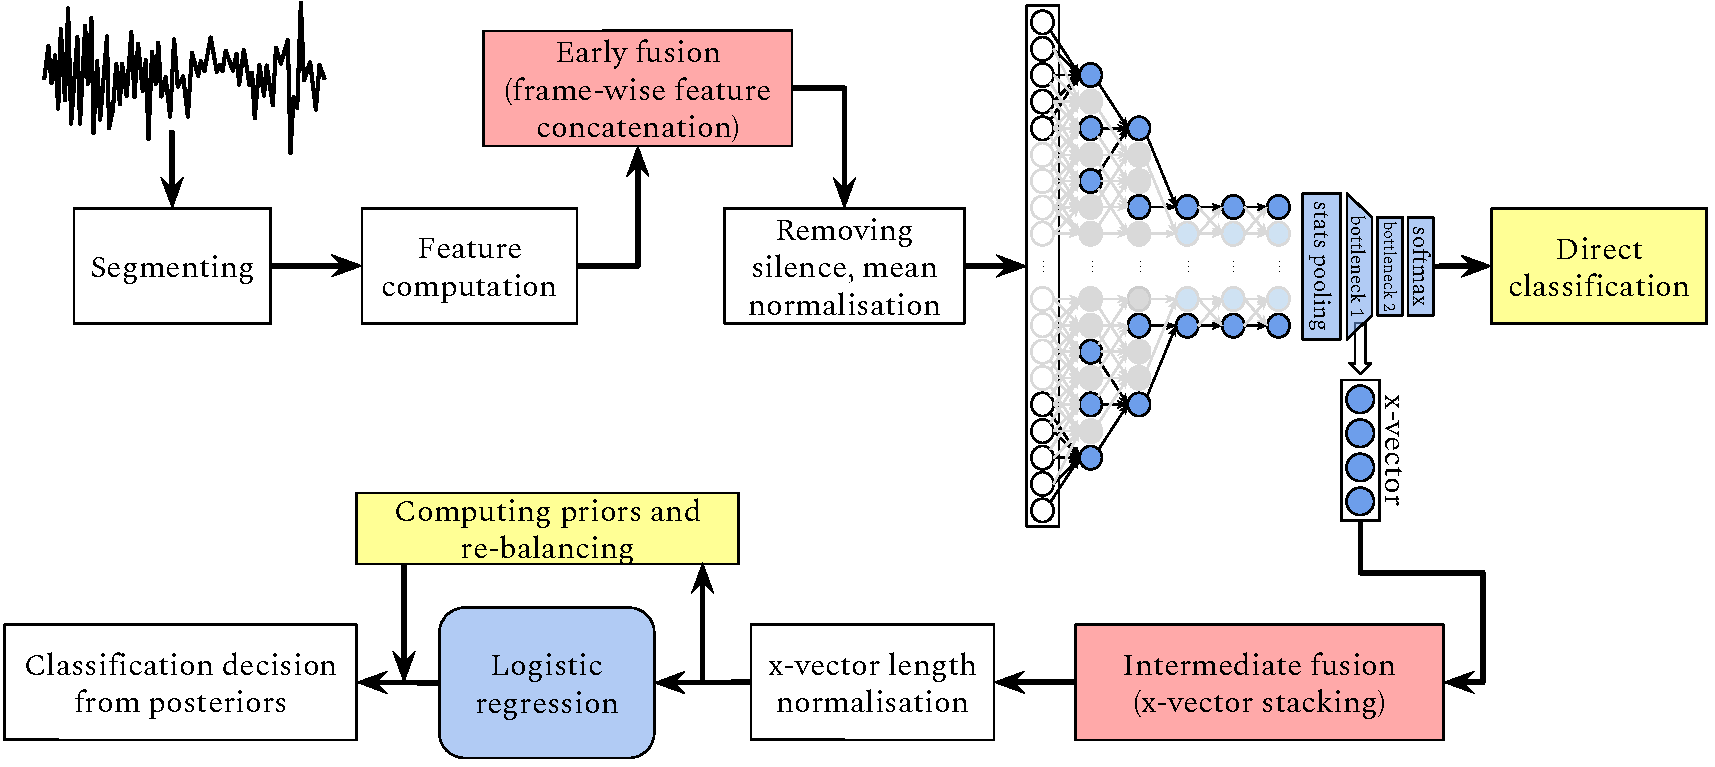
\includegraphics[width=15cm]{graphics/architecture}
      \vspace*{-1em}
      \caption{An end-to-end overview of my system. Note that the segmenting step does not apply to the x-vector TDNN training data. The fusion steps which can be omitted are highlighted in red while yellow marks the steps only performed at training time.}
      \label{fig:architecture}
    \end{figure}

    % TO-DO: mention that implementing this end-to-end thing took the most time and running experiments was really fast

    \autoref{fig:architecture} shows the entire system and what the main steps in running it are. In what follows, I elaborate on each step that has not been described yet.

    \subsection{Feature computation}{
      \label{sec:feature-computation}
      % data preparation
      %   feature computation
      %   - existing scripts re-used for computing MFCCs (make\_mfcc.sh), I adapted the code for adding SDCs and deltas to MFCCs
      %   - existing scripts re-used for adding pitch
      %   - energy feature computed simply as a special case of MFCC: taking only 0th coefficient and using raw log energy instead of it
      Throughout my experiments, the following feature types are used (as a refresher, see \autoref{sec:features}): MFCC, MFCC+$\Delta$+$\Delta\Delta$, SDC, energy, and Kaldi pitch. For more details, see (TO-DO: link the experiments section where the dimensionalities of these are explained).

      To enable frame-wise feature concatenation, all feature types were computed with the same frame width of 25ms and frame shift of 10ms. Windowing was done using the Povey window\footnote{the default windowing function in Kaldi, defined and implemented here: \url{https://github.com/kaldi-asr/kaldi/blob/master/src/feat/feature-window.cc\#L109}}, a slight variation of the commonly used Hamming window \citep[p. 200]{Blackman_Tukey_1958}; see \autoref{fig:window-types} for a comparisons.
      \begin{figure}[h!]
        \centering
        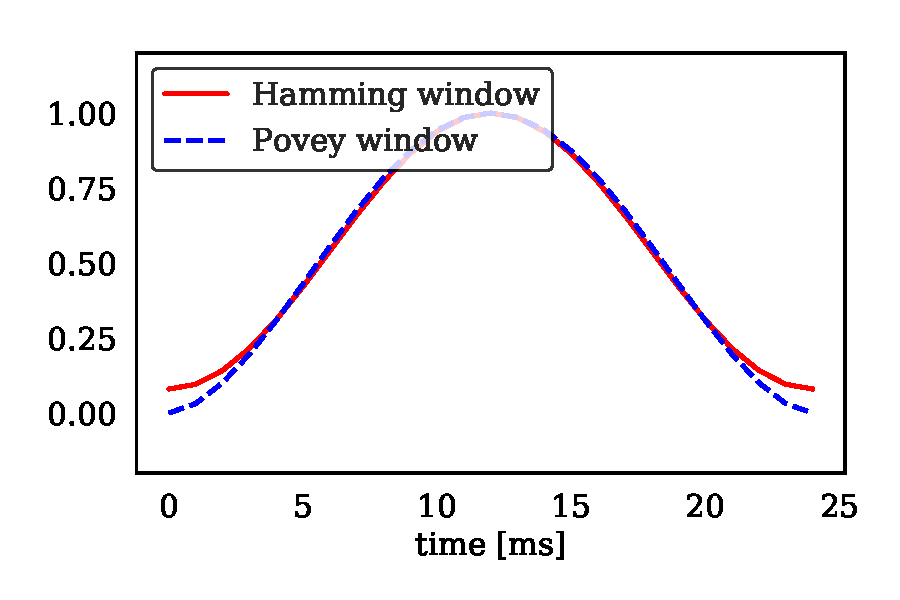
\includegraphics[width=9cm]{../img/window-types.pdf}
        \vspace*{-1em}
        \caption{Comparison of the Hamming and Povey tapered windowing functions on a frame of length 25ms. (The frame length, however, does not make a difference, it is the different shapes of the windows that matter.)}
        \label{fig:window-types}
      \end{figure}

      While MFCC features were computed using the existing script \verb|steps/make_mfcc.sh|, I adapted the script in order to conveniently compute the SDCs, MFCCs with deltas, and the Kaldi pitch. The energy feature was computed as a special case of the MFCC feature -- by computing the raw log energy instead of the 0\textsuperscript{th} cepstral coefficient, and discarding all remaining cepstral coefficients.
    }

    \subsection{Early fusion}{
      \label{sec:early-fusion}
      % TO-DO: Maybe introduce fusion earlier??
      % early fusion
      % - I wrote script for frame-wise concatenation
      % - done for all data partitions alike
      % - 3s mean normalisation before x-vector extraction and also for tdnn training samples -- for all feature types
      By fusion I understand simply combining multiple sources of information -- be it early utterance representations (feature vectors of different feature types), intermediate representations (in this case x-vectors) or even scores from multiple classifiers (perhaps each trained on x-vectors based on a different feature type).
      Early fusion here means combining the different feature types as early as possible in the whole pipeline: right after feature computation. For a simple example of early fusion see \citet{Martinez_et_al_2012} who concatenate for each short speech segment the information about the pitch contour, the energy contour, and the voiced region duration. In this case, I created a script for frame-wise concatenation (splicing) two or more feature vectors for a given utterance. Such precise alignment was possible because I configured all feature types to be computed with the same frame length and frame shift.
    }

    \subsection{Feature vector post-processing}{
      \label{sec:feature-postprocessing}
      % removing silence with VAD from MFCCs
      % mean normalisation
      This comprises two steps unchanged from the SRE16 recipe and used in the x-vector LID paper \citep{Snyder_et_al_2018}:
      \begin{enumerate}
        \item {Removing frames containing silence, using the voice activity decision (VAD). The only difference with respect to the SRE16 recipe is that the VAD is computed only once -- using the MFCC features -- and used for these and all other feature types (see also \autoref{sec:preprocessing}).}
        \item {Mean-normalisation is performed by subtracting from each frame the mean over the surrounding 3s window. This is a technique commonly used for processing acoustic features. It preserves relative temporal trends in feature values and discards information about the absolute values. I decided to use it for all prosodic features as well. However, it is possible that capturing tone properties for languages with register tonal systems -- i.e. those that mark tone using several flat tone \textit{levels} instead of characteristic tone \textit{shapes} -- would better be realised by preserving the absolute values (without mean normalisation).}
      \end{enumerate}
    }

    \subsection{The x-vector TDNN}{
      \label{sec:x-vector-tdnn}
      % - architecture as described in \autoref{sec:x-vectors}, no changes to the code from the recipe
      Even though this part of the architecture was adapted from the SRE16 recipe without any major changes and is available as an open source, I still provide a description to help the reader appreciate the technical realisation of the core of an x-vector system. (Adding to what I wrote in \autoref{sec:d-vectors} and \autoref{sec:x-vectors}.)

      % ARCHITECTURE
      % - number of parameters: 4.6M (MFCC+deltas+pitch+energy) to 4.4M (energy)
      The TDNN's layers are described in \autoref{tab:x-vectors}; the network had 4.4-4.6M parameters (depending on the dimensionality of the input feature vectors). Each layer used the rectified linear unit (ReLU) activation function.

      % TRAINING DATA: iterations, epochs, minibatches
      % - utts <5s (500 frames) removed from training data
      % - training data repeated 35 times, distributed into archives of roughly 50000000 frames each (around 140h). 70 training archives
      % - number of epochs translated into a number of iterations (each iteration = one archive)
      % - samples globally shuffled before training, then shuffled each iteration within batches of 1000
      As for the handling of the training data, the first step was discarding utterances shorter than 5s. Looking back, this design decision of \citet{Snyder_et_al_2018} may have been challenged as it resulted in discarding 29\% of my total number of training utterances. However, the effects of using very short training segments might potentially have a negative impact on the TDNN. After discarding short utterances, the rest of the training data was replicated 35x, randomly shuffled and distributed and saved into 70 training Kaldi archives, each archive corresponding to a training iteration and containing roughly 50,000,000 frames (feature vectors) each -- around 140h of speech. This way, each training epoch consisted of processing 70 archives, which, however, translates to only 23 actual iterations as the training was using 3 parallel jobs, each processing one archive per iteration (see bellow for a description of the parallel training). The archives were processed in minibatches of 64 utterances, every minibatch shuffled in each iteration.

      % TRAINING: objective function, learning algorithm
      % - optimising multi-class cross-entropy     
      In the training phase, the TDNN was trained to directly classify each utterance as one of the 19 languages, the training objective function being multi-class cross-entropy.
      % batch normalisation. maximum parameter change: The maximum change in parameters allowed per minibatch, measured in Euclidean norm over the entire model (change will be clipped to this value): 2.0.
      Each layer was using batch normalisation and, to prevent extreme parameter updates, the maximum parameter change per minibatch -- measured as the Euclidean norm over the entire parameter vector of the network -- was clipped to 2.0.
      % - corresponds to that described in \citet{Snyder_et_al_2018}: NG-SGD training with EFFECTIVE lr exponentially decreasing from 0.001 to 0.0001, described in \citet{Povey_et_al_2014} (also:  Trained with 3 parallel jobs, parameter shrinking and with momentum with the momentum-term coefficient $\mu=0.5$ described therein), dropout scheme is 0 (at 0\%-20\%), 0.1 (at 50\%), 0 (at 100\%). Backstitch is NOT used.
      The training uses several techniques developed or empirically found to be beneficial by the John Hopkins University team. (Most them are mentioned or summarised by \citet{Povey_et_al_2014}, even though the paper corresponds to the \verb|nnet1| neural network implementation in Kaldi, while the SRE16 recipe uses the newer \verb|nnet3| implementation (which contains some additional improvements).) The learning rule is the Natural gradient Stochastic gradient descent (NG-SGD) with momentum (using the coefficient of momentum value of 0.5), with the learning rate exponentially decaying across the training iterations from 0.001 to 0.0001. As a means of regularisation, weak dropout was used, with the dropout rate varying according to the following schedule: 0 for the first 20\% of training iterations, then increasing linearly to 0.1 for the following 30\% and finally decreasing linearly until the value of 0 in the last iteration.
      Perhaps most importantly, the training was realised using 3 parallel jobs, hence speeding it up. The parallelisation translates into 3 model instances being run in parallel and their parameters synchronised (averaged) after each iteration (for mode details, see \citeauthor{Povey_et_al_2014}). Note that the SRE16 recipe varied the number of parallel jobs throughout training linearly from 3 to 8, but the constant 3 jobs better suited my computational environment, hence I made this change to the SRE16 implementation.

      As a side note, even though the TDNN is presented as processing variable-length utterances, it still has an upper limit on the utterance length given by the implemented maximum temporal context over which the convolutional filters of its first layer slide: 1000 frames (roughly 10s when using the standard frame shift of 10ms). This means that utterances longer than 10 seconds were split and processed separately. When using the trained TDNN for extracting x-vectors, a long utterance could this way result in multiple x-vectors. This, however, did not apply to my evaluation and testing data as those were segmented into utterances of maximum length 10s.
      
      In terms of runtime, training the TDNN was the most time-consuming step: It took 19 hours (for details, see \autoref{sec:hyperparameters}).
    }

    \subsection{Extracting x-vectors}{
      \label{sec:extracting-x-vectors}
      % - 512-D x-vectors
      In this step, 512-dimensional x-vectors were extracted for all enrollment utterances (to train the classifier), and for evaluation and testing utterances (to evaluate the system end-to-end).
      % extracting x-vectors
      % - done using the sre16 code without any changes
      % - ignoring utts <1s
      This step was adapted from the SRE16 recipe with only one change: I implemented discarding all utterances that were shorter than 100 frames (roughly 1s). I decided to implement this thresholding partly to not use segments that are unrealistically and unfairly short (compare with the typical length of 3s, 10s or even 30s), but also to address the issue of a small number of extremely short or corrupt audio files which were causing the Kaldi pitch-tracking binary to fail.

      % - takes around 1.5h for enroll, eval and test data combined (when using 32 parallel jobs)
      % - have: 17212 30s enrollment segments + 20349 10s eval segments + 18710 10s test segments => around 100ms per segment (to produce x-vector)
      This step was relatively time-consuming: around 1.5h for the enrollment, evaluation and testing data combined when splitting the work into 32 jobs and running them 10 at any time (the limit of 10 given by the computing environment's limit on the number of Slurm jobs, see \autoref{sec:computing-environment}). Still, given the number of segments to be processed, the per-segment time is very low. With evaluation and testing segments being up to 10s long, I had 17212, 20349 and 18710 segments for enrollment, evaluation and testing, respectively, and the per-segment time was thus only around 100ms.
    }

    \subsection{Intermediate fusion}{
      \label{sec:intermediate-fusion}
      % intermediate fusion
      % - I wrote script for concatenating 2 or 3 x-vectors together for each utterance, resulting in 1024-D or 1536-D x-vectors
      Intermediate fusion, as opposed early fusion, combines utterance-level (not frame-level) representations (x-vectors) produced by multiple (up to 3) different x-vector TDNNs. The x-vectors are concatenated, creating a longer vector. In my case, the different networks would have been trained on different feature types, and the fused vectors would be 1024- or 1536-dimensional.

      The script for this step was written by me as the intermediate fusion is both an easy to implement and a seldom used strategy -- typically, \textit{late} fusion is performed, i.e. combining the final scores from different classifiers (see, for example, \citet{Snyder_et_al_2018,Martinez_et_al_2012}).
    }

    \subsection{The classifier}{
      \label{sec:classifier-description}

      As mentioned earlier, the multi-class logistic regression classifier trained to optimise multi-class cross-entropy was chosen and adapted from the LRE07 recipe. I adapted the scripts such that training and scoring could be done separately. This way, both the TDNN and the classifier could be trained, then evaluated end-to-end on the evaluation set used in turn to optimise the hyperparameters of the classifier, and finally the system would be used to only score the testing set utterances.

      % - whitening or dimensionality reduction is not performed
      % - all vectors length-normalised before fed into classifier!
      Importantly, the whitening and dimensionality reduction steps employed by \citet{Snyder_et_al_2018} were omitted as I deemed them important for their particular classifier set up, but not necessarily mine. I decided to only keep the one preprocessing step that was included in the LRE07 recipe: length-normalising the vectors before being processed by the classifier.

      Perhaps the most interesting aspect of the classifier is the possibility to use it as a mixture model. Even though this functionality is open-sourced and built right into the \verb|logistic-regression-train| Kaldi binary, I explain it so that the reader can appreciate the capabilities of the classifier as well as my later hyperparameter tuning. 
      %   - max-steps: Maximum steps in L-BFGS (default: 20).
      %   - normalizer: Coefficient for L2 regularization (default: 0.0025).
      %   - power: Power rule for determining the number of mixtures to create (default: 0.15).
      %   - mix-up: Target number of mixture components to create (default: 0).    
      In order to train the classifier, one provides the following parameters: \verb|max-steps| (the maximum number of iterations of the L-BFGS solver in training the model), \verb|normalizer| (the L2 regularisation coefficient), \verb|mix-up| (the desired number of decision boundaries used to model all classes), and \verb|power| (explained later). Then, training the model comprises the following steps:
      \begin{enumerate}
        % - first trained for max-steps with number of classes = K (19)
        \item {Train the classifier normally with $L$ decision boundaries ($L=19$ being the number of classes) for \verb|max-steps| iterations.}
        % - then split each class into a number of "sub-classes" like a mixture model. done iteratively, in each iteration splitting the biggest cluster into two. what 'biggest' means is determined by the 'power' parameter: $(total-occ^power)/num-components$ is taken as the adjusted per-component occupancy of the cluster, thus using using power closer to 0 means that the number of components will be more equal across all classes, whereas for big power (close to 1) big classes will be split into many more components than smaller classes
        \item {Determine which classes will be modelled by how many decision boundaries -- attempting to end up with \verb|mix-up| or fewer boundaries. In general, no class is modelled by more decision boundaries than the number of corresponding training samples, and bigger classes are modelled by more boundaries. Starting with $L$ boundaries, iteratively, this number is incremented: In each iteration, the class currently with the biggest per-boundary occupancy is granted another boundary, where the per-boundary occupancy of class $l$ is:
        $$\frac{
                (\textrm{number\ of\ training\ samples\ for\ class }l)^{\mathtt{power}}
               }{\textrm{number of boundaries for class }l}$$
        Notice how the \verb|power| parameter (when set to a value closer to 0) can effectively bring the class sizes closer together, thus causing the number of boundaries to vary less with class sizes. Values closer to 1.0 (or bigger), on the other hand, cause bigger classes to be modelled by many more boundaries than small classes.
        }
        % - then trained for another max-steps but with number of classes corresponding to mix-up. the decision boundaries are initialised from the K decision boundaries with some added random noise so they would differ slightly. essentially, each class is modelled using multiple decision boundaries but all boundaries (mixture components) have the same weight
        \item {Clone the trained boundary from step 1 to create as many boundaries for each class as determined in step 2; adding some random noise to each clone to ensure that the added boundaries are distinct but still roughly based on the original boundary.}
        \item {Train the extended model (now with up to \verb|mix-up| boundaries) for additional \verb|max-steps| iterations.}
      \end{enumerate}

      The trained classifier is then used to compute the posterior probability for a given x-vector $x$ and a particular class $l$, by accumulating the contributions across the set of boundaries $B_l$ modelling the given class, and scaling by the class prior $p(l)$:
      \begin{equation}
        \label{eq:logit-posterior}
        p(l|x) \approx p(l)\sum_{b \in B_l} p(x|b)
      \end{equation}
      Subsequently, $x$'s predicted class is taken to be the one with the maximum posterior.

      % - rebalancing priors: $(count(lang-test) / count(lang-train) )^(prior-scale)$ where prior-scale=0.7 (same as in the original LRE07 recipe, and generally recommended values are between 0.5 and 1.0)
      As mentioned in \autoref{sec:data-overview}, the enrollment set was imbalanced and some languages were over-represented while others were under-represented. The mechanism used in the LRE07 recipe to cope with such imbalance is computing scaling factors for the different languages and using these for re-balancing the classifier's priors after it has been trained. Given a value (typically between 0.5 and 1.0) of the parameter $s$, the prior for language $l$ will be scaled by coefficient $c$ computed as follows:
      \begin{equation}
        \label{eq:logit-prior}
        c_L = \bigg( \frac{C_{l, evaluation}}{C_{l, enrollment}} \bigg)^s
      \end{equation}
      where $C$ are the counts of utterances in language $l$ in the respective data sets. In other words, if the distribution of languages in the enrollment set matches that in the evaluation set, all priors will be scaled by the same factor -- effectively not being scaled -- and the classifier's priors will reflect the distribution observed in the enrollment set. However, if the distributions do not match, the classifier's priors (driven by the enrollment set) will be corrected in the direction indicated by the distribution in the evaluation set. Of course, the evaluation set does not necessarily correctly reflect the language distribution in unseen data. Hence, by setting the $s$ parameter to a value smaller than 1.0, correcting the priors can be made less reliant on the evaluation set's distribution.
      I keep the value of $s=0.7$ as used in the LRE07 recipe -- particularly because this is not a parameter that could be tuned given one's data, only set to an empirically trusted value. The scaling factors used for rebalancing the classifier (in the 10s condition) are shown in \autoref{fig:logit-priors}. Clearly, languages such as Arabic and Croatian were identified as under-represented and the classifier will be re-balanced to prefer them more. The opposite goes for Japanese or Vietnamese.
      % - add graph showing distribution of priors and eval utt counts
      \begin{figure}[h!]
        \centering
        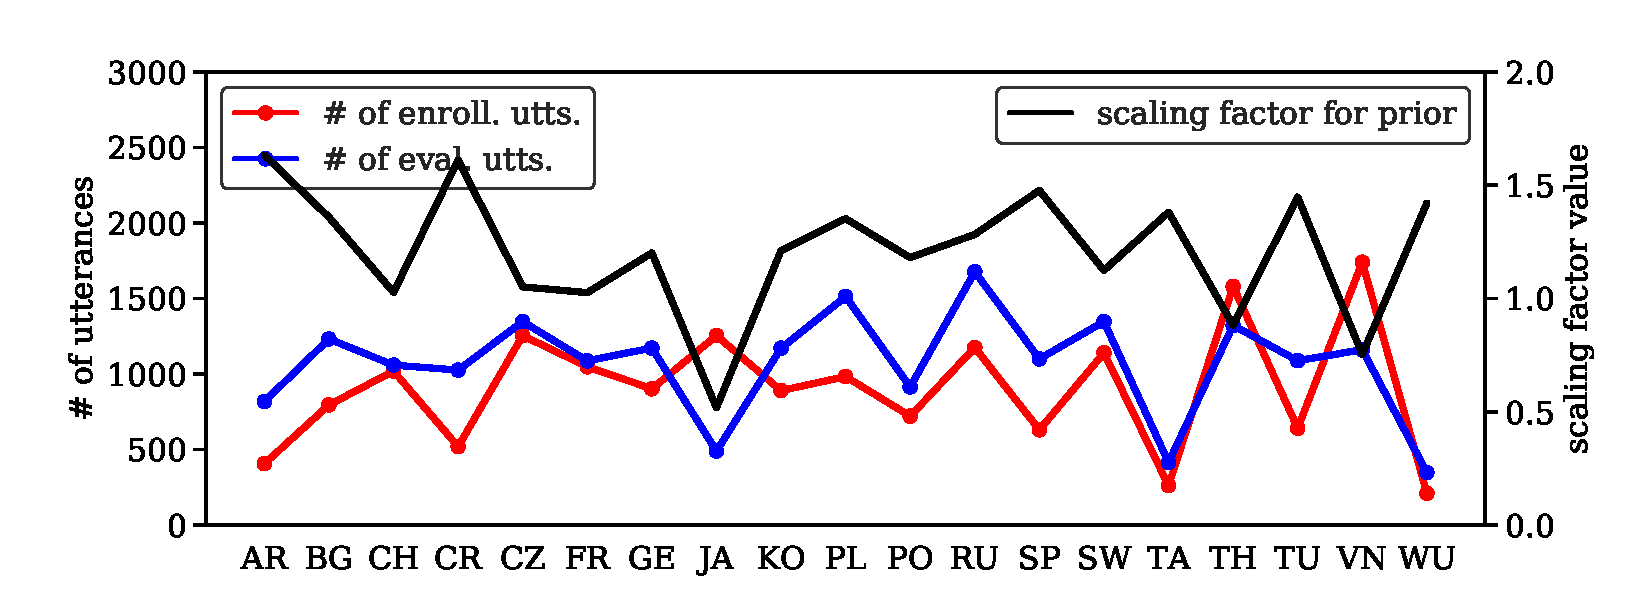
\includegraphics[width=15cm]{../img/logit-priors.pdf}
        \vspace*{-1em}
        \caption{Scaling factors used for adjusting the classifier's priors based on the language distributions in the enrollment and evaluation set.}
        \label{fig:logit-priors}
      \end{figure}

      Compared to training the TDNN, training the classifier (with the hyperparameter values found in \autoref{sec:hyperparameters}) takes only around 3.5 minutes (in the 10s condition). Producing posteriors and computing the final results for the entire test set takes only around 4 seconds (using a single CPU), corresponding to inference time of only $\sim$0.2ms/utterance.
    }
  }

  \section{Computing environment}{
    \label{sec:computing-environment}
    % the School of Informatics student GPU cluster
    All experiments were carried out in the School of Informatics' Teaching cluster\footnote{\url{http://computing.help.inf.ed.ac.uk/teaching-cluster}}, using GPUs model GeForce GTX 1060 6GB, and CPUs model Intel Xeon E5-2620 v4 (2.10GHz). Note that the GPUs were only used in training the x-vector TDNN and in extracting x-vectors from the trained network -- the two most time-consuming stages.
    
    % - used for training and extracting x-vectors
    % CPUs were:  Intel(R) Xeon(R) CPU E5-2620 v4 @ 2.10GHz
    % Slurm job scheduler
    % using one GPU per parallel job (i.e. 3 GPUs in TDNN training)
    % talk about why changing 3..8 to 3..3 enabled me to train 3 experiments in parallel, etc. also, refer to kaldi-help where this was discussed
    For running jobs requiring GPUs, the Slurm scheduler was used, configured such that a single user like me could only ever run at most 10 Slurm jobs at the same time. As a result of this restriction, in order to speed up my experiments, I set the number of parallel jobs used to train each x-vector TDNN to 3 -- so that I could train as many as three TDNN networks in parallel. While the SRE16 recipe uses more jobs, decreasing this number could only help the quality of the final model\footnote{as hinted by Dan Povey at \url{https://groups.google.com/forum/\#!topic/kaldi-help/_iyJP-lHkKM}}.
    Note that each Slurm job was allocated a separate GPU. Thus, each TDNN can be considered to have been trained using three GPUs of the abovementioned model.
  }

  \section{Hyperparameters}{
    \label{sec:hyperparameters}

    The aim of this work is not to extensively tune the hyperparameters of the architectures; instead, I rely on values used in previous successful works of others (provided in the adapted recipes). However, there was a number of parameter which I decided to change or even fine-tune.

    As discussed previously, I changed the number of parallel jobs used by the TDNN in its training, and imposed a minimum length on any utterances for which x-vectors would be extracted.

    % LRE07 settings
    % --max-steps=35
    % --normalizer=0.001
    % --verbose=3
    % --power=0.15
    % --mix-up=150
    % DEFAULTS
    %   - max-steps: Maximum steps in L-BFGS (default: 20).
    %   - normalizer: Coefficient for L2 regularization (default: 0.0025).
    %   - power: Power rule for determining the number of mixtures to create (default: 0.15).
    %   - mix-up: Target number of mixture components to create (default: 0).   
    After initially training the TDNN for 3 epochs and seeing that it took over 8 hours, I decided to first tune the classifier's hyperparameters. This way, the tuned classifier could be subsequently used for end-to-end evaluation of different TDNNs, enabling the tuning of the most important hyperparameter: $E$ -- the number of training epochs of the TDNN. As discussed previously, the classifier's hyperparameters were \verb|max-steps|, \verb|mix-up|, \verb|normalizer| and \verb|power|. The last mentioned parameter I fixed to be of the default value 0.15 (also used by the LRE07 recipe) -- meaning that the number of decision boundaries was only weakly dependent on the relative class size (in terms of the number of enrollment segments). The other three parameters were tuned using enrollment and evaluation x-vectors extracted from the baseline-case TDNN (i.e. using MFCC features and 10s enrollment segments) trained for 3 epochs. I carried out a 3-dimensional grid search, exploring the following value ranges: 
    \begin{itemize}
      \item{\verb|max-steps| $ \in \{20, 40, 60, 80, 100, 120, 140, 160, 180, 200\}$ (the default is 20, the LRE07 recipe uses 35)}
      \item{\verb|mix-up| $ \in \{19, 50, 100, 150, 200, 250, 300\}$ (the default is 0, the LRE07 recipe uses 150 for 14 languages)}
      \item{\verb|normalizer| $ \in \{0, 0.00001, 0.0001, 0.001, 0.01\}$ (the default is 0.0025, the LRE07 recipe uses 0.001)}
    \end{itemize}
    \begin{figure}[h!]
      \centering
      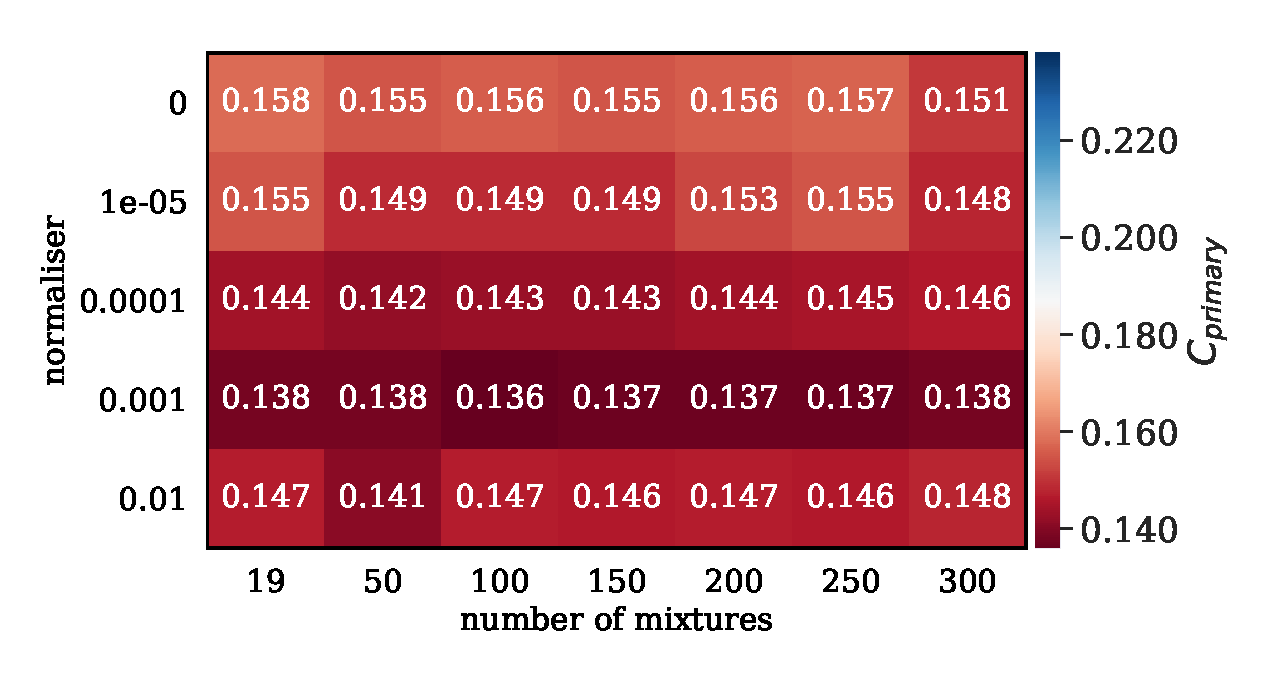
\includegraphics[width=11cm]{../img/normaliser_vs_mix-up_best.pdf}
      \vspace*{-1em}
      \caption{Evaluation set $C_{primary}$; the shown value is the best one across all explored values of the \texttt{max-steps} parameter.}
      \label{fig:normaliser_vs_mix-up_best}
    \end{figure}
    \autoref{fig:normaliser_vs_mix-up_best} shows the best result across all numbers of training iterations for each combination of \verb|mix-up| and \verb|normalizer|, showing rather clearly that \verb|normalizer|=0.001 (also used by the LRE07 recipe) is the optimal value within the explored range.
    \begin{figure}[h!]
      \centering
      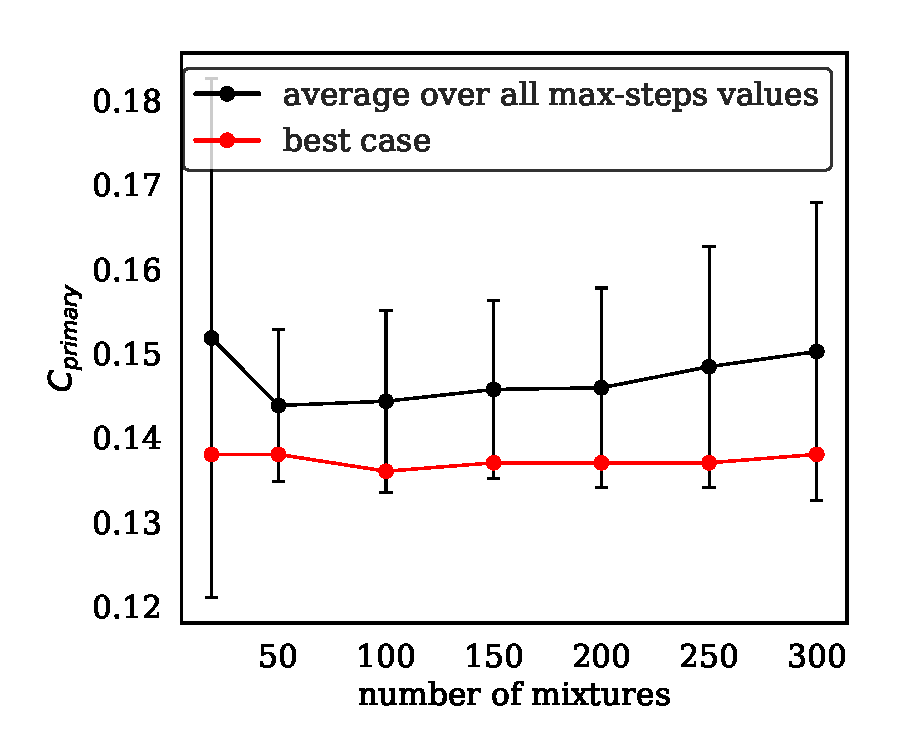
\includegraphics[width=8cm]{../img/logit_mix-up.pdf}
      \vspace*{-1em}
      \caption{Evaluation set $C_{primary}$ varying with the number of mixture components of the classifier.}
      \label{fig:logit_mix-up}
    \end{figure}
    \begin{figure}[h!]
      \centering
      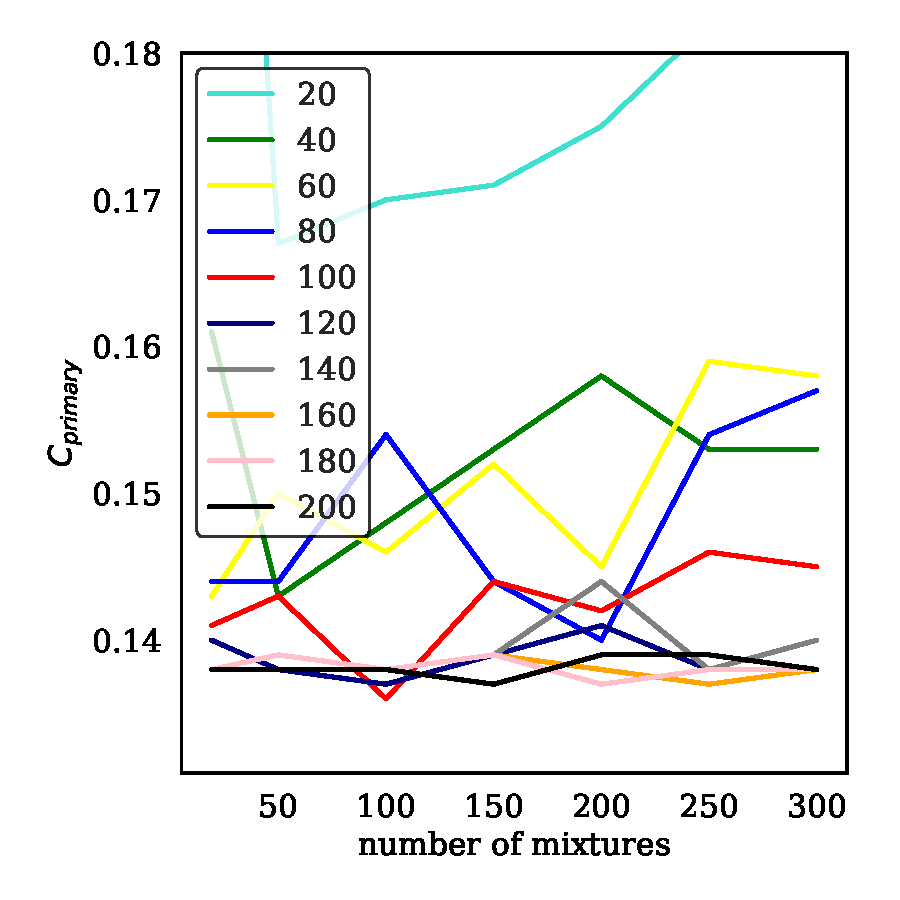
\includegraphics[width=8cm]{../img/logit_max-steps_vs_mix-up.pdf}
      \vspace*{-1em}
      \caption{Evaluation set $C_{primary}$ varying with the number of mixture components for each explored number of training steps.}
      \label{fig:logit_max-steps_vs_mix-up}
    \end{figure}
    Fixing this parameter and plotting just the performance against the number of mixture components \verb|mix-up| (see \autoref{fig:logit_mix-up}) led me to the conclusion that \verb|mix-up| should be chosen as 50 or 100. Further plotting the performance as varying with the number of mixture components for each number of training iterations separately (\autoref{fig:logit_max-steps_vs_mix-up}) shows how not just worse but also unstable the performance is for lower number of iterations. Thus, I decided to use \verb|max-steps|=200 and -- even though it seems to not make a big difference -- I fixed \verb|mix-up| at the best performing value of 100.

    Then, I tuned $E$. In particular, I wanted to reach a reasonable compromise between too long training runtimes and too low evaluation set performance. $E$ was tuned in the baseline condition, i.e. using MFCC features and 10s evaluation segments. The system was evaluated end-to-end, using the optimal values of the classifier established above. The results are summarised in \autoref{fig:num-epochs}. Clearly, the early epochs are the most important, but the performance (in terms of $C_{primary}$) also plateaus fairly quickly: beyond 10 training epochs and, when measured by accuracy, it even starts becoming worse, indicating that the TDNN probably starts to overfit the training data. AS the compromise value of $E$, I decided to use the "elbow" point of the $C_{primary}$ plot in \autoref{fig:num-epochs}, where $E=7$. This implies the training runtime of around 19 hours to train a single x-vector TDNN.
    \begin{figure}[h!]
      \centering
      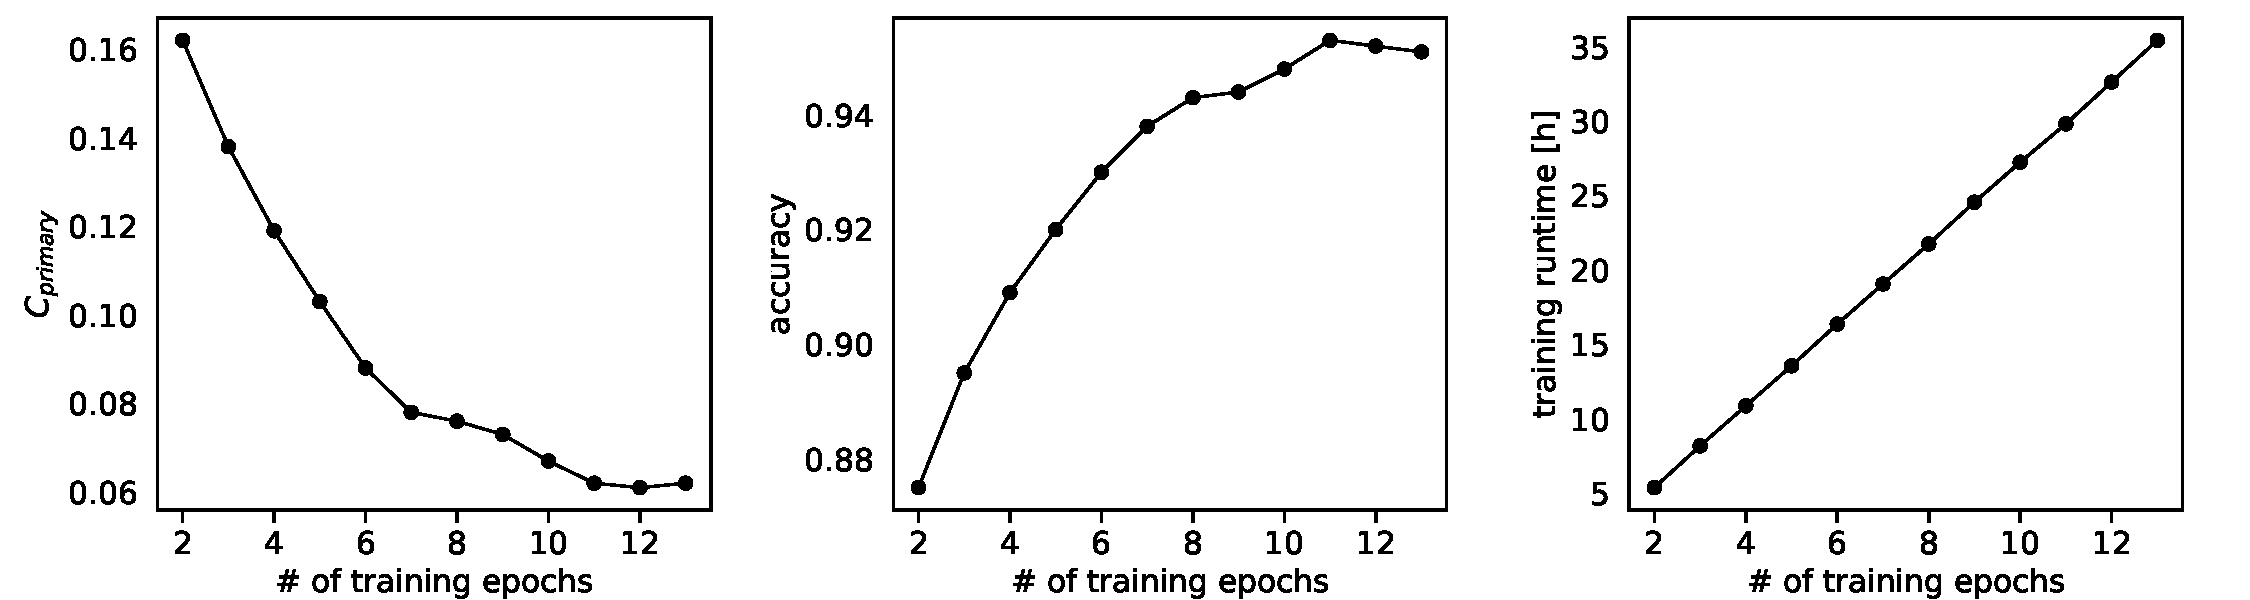
\includegraphics[width=14.9cm]{../img/num-epochs.pdf}
      \vspace*{-1em}
      \caption{Evaluation set performance and training runtime for varying number of training epochs $E$ of the TDNN.}
      \label{fig:num-epochs}
    \end{figure}
  }
}

% TO-DO: mention and explain C-primary and why I use it!
\chapter{Experiments and discussed results}{
  \label{chap:Experiments}

  In this chapter, I describe the experiments that I carried out, in the order they were designed. I provide raw results followed by a discussion of the experiment. For overall discussion, focusing more on relating my work to past studies and suggesting the directions for further research, see \autoref{chap:discussion-and-conclusions}. However, my ability to compare my results with those of others is limited: To the best of my knowledge, this is the first work using the GlobalPhone corpus for LID, and the commonly used NIST LRE corpora differ in many ways (as discussed in \autoref{chap:Data}).

  The aims of my experiments can be summarised into the following key points:
  \begin{enumerate}
    % - compare acoustic feats, see if deltas or context aggregation with SDCs can help (TDNN should be able to do it on its own)
    \item {Compare the different types of acoustic features in the context of the x-vector system. Dynamic features -- be it simple delta terms or the more sophisticated SDCs -- were designed primarily to help frame-level models to capture temporal contexts. The x-vector TDNN, on the other hand, does capture such contexts explicitly. Therefore, a question I ask is whether the more sophisticated acoustic features can still improve performance compared to simple MFCCs.}
    
    % - see how prosodic features on their own perform, and also combined (early and intermediate fusion)
    \item {Evaluate the usefulness of prosodic features alone. Even though there is no good reason to use only the prosody (i.e. to not consider acoustic features at all), I believe that building a system that uses only prosodic features can help me better understand and analyse the nature and value of the prosodic information.}
    
    % - see how well prosodic+acoustic features work (early and intermediate fusion)
    \item {This is my ultimate aim: to evaluate the effect of using both acoustic and prosodic information -- combined in different ways.}
  \end{enumerate}

  % Evaluation metric: $C_{primary}$, consistent with NIST LREs (TO-DO: mentioned in an earlier section?). I also report confusion matrices and accuracy as these are easier to intuitively reason about and analyse.
  Throughout all experiments, I use $C_{primary}$ as the main metric -- staying consistent with the latest LRE 2017 challenge and the work of \citet{Snyder_et_al_2018}. In the tables with results, the best result in terms of the $C_{primary}$ value is always put in bold face. Additionally, I also report accuracy and later show confusion matrices as these are easier to intuitively grasp and reason about.

  \section{The setup}{
    \label{sec:exp-setup}
    % definitions of features (dimensionalities)
    As for the feature type, the default was the MFCC features of 23 dimensions without energy (same as \citet{Snyder_et_al_2018}). The other two acoustic features were derived from the computed MFCCs and designed such that their dimensionalities would be roughly the same (for a fairer comparison):
    \begin{itemize}
      \item {the MFCC+$\Delta$+$\Delta\Delta$ features were 69-dimensional, using 23 first-order and 23 second-order delta terms,}
      \item {the SDC features were 72-dimensional, using the 9-1-3-7 configuration, i.e. computed at 7 locations using the first 9 cepstral coefficients and discarding the rest of the coefficients.}
    \end{itemize}
    I made the decision to compute the MFCC features using the Kaldi default of 23 Mel filters, and on the frequency range of 20-7800Hz inspired by the Kaldi manual\footnote{\url{http://kaldi-asr.org/doc/feat.html\#feat_mfcc}}.

    As for the prosodic features, the energy was computed from the MFCCs and was simply a 1-dimensional feature vector per frame. The Kaldi pitch was 5-dimensional, computed using the default parameter values of the Kaldi \verb|compute-kaldi-pitch-feats| binary, in particular using $B=7000$ (see \autoref{eq:nccf}), the penalty factor for frequency jumps of 0.1, and \verb|min-f0|$=50$Hz. I changed the \verb|max-f0| from the default of 400Hz to 500Hz, same as the upper $F_0$ limit used by \citet{Lin_et_al_2005}.

    In addition to the default 10s condition (i.e. testing segments being of length $\leq10\textrm{s}$), I also evaluate the systems on $\leq3$s testing segments (the 3s condition). On these shorter segments, the systems will certainly perform worse, but the results are important because optimising LID performance on short segments is valuable and important for: online processing (where we want to identify the language as soon as possible), low-resource settings, settings with frequent code switching, and similar scenarios where the segment to be processed is very short.
  }

  \section{Comparing acoustic features}{
    \label{sec:exp-acoustic}

    In this experiment, I compare systems trained on the three types of acoustic features and evaluated on the testing segments in both the 10s and the 3s conditions.

    % MFCC & 0.0660 & 0.9426 & 0.1477 & 0.8746 \\
    % MFCC+$\Delta$+$\Delta\Delta$ & 0.0567 & 0.9522 & 0.1380 & 0.8855 \\
    % SDC & 0.0543 & 0.9526 & 0.1575 & 0.8677 \\
    \begin{table}[h!tb]
      \centering
      \begin{sc}
        \footnotesize
        \begin{tabular}{l|cc|cc}
                  & \multicolumn{2}{c|}{10s}  & \multicolumn{2}{c}{3s} \\
          feature & $C_{primary}$ & accuracy & $C_{primary}$ & accuracy \\
          \hline
          MFCC & 0.0660 & 0.943 & 0.148 & 0.875 \\
          MFCC+$\Delta$+$\Delta\Delta$ & 0.0567 & 0.952 & \textbf{0.138} & 0.886 \\
          SDC & \textbf{0.0543} & 0.953 & 0.158 & 0.868 \\
        \end{tabular}
      \end{sc}
      \caption{Comparing the systems trained on acoustic features.}
      \label{tab:results-acoustic}
    \end{table}

    The results are presented in \autoref{tab:results-acoustic}. Just looking at the accuracy values (all above 85\%), all systems perform very well (remember that naive majority class guessing would yield accuracy of only roughly $1/19=5.3\%$).
    % context of MFCC: 15f, MFCC+deltas: 19f, SDC: 3x(7-1)+15=33
    % deltas improve performance by 14\% (7\%), sdcs by 18\% (worse by 7\%)
    Clearly, both simple deltas and SDCs improve on the performance achieved by simple MFCCs in the 10s condition -- in this case by 14\% and 18\%, respectively. The relative gain is smaller in the 3s condition. 
    % one might think that dynamic feats won't help much
    % dynamic feats were designed to mitigate the limitations of frame-level systems
    % but widening the temporal context seems to still help
    The observed improvement answers my earlier question about the usefulness of dynamic features in the era of models which process sequences of frames: Clearly, these features still have something to offer. If nothing else, extending the temporal context by the means of dynamic features may remain a computationally cheaper alternative to increasing the context by changing the TDNN architecture.

    Interestingly, SDCs make the performance worse in the 3s condition. I hypothesise that this can be attributed to the relatively big temporal context of SDCs. To compute the SDC feature vector for a frame, a context of -1 and +19 frames\footnote{for a $N$-$d$-$p$-$k$ SDC configuration, the context is -$d$ and +$(p\times(k-1)+d)$} is required, while computing the simple deltas only requires a context of $\pm$2 frames. This means that -- for a $\leq$3s segment -- a big portion of the SDC vectors will be only partially computed: For a 200-frame segment (roughly 2s), the SDCs are incomplete for 20 frames (10\%) while MFCC+$\Delta$+$\Delta\Delta$ will be incomplete only for 4 frames (2\%). Although this hypothesis would require further research, for now I conclude that, for very short segments, dynamic features computed over long contexts should be used with care. Ideally, features requiring shorter contexts -- such as simple deltas or even MFCCs without deltas -- would be used.    
  }

  \section{Comparing and combining prosodic features}{
    \label{sec:exp-prosodic}

    This experiment focuses on comparing systems trained on the two prosodic features, as well as systems where the Kaldi pitch and energy was combined via early and intermediate fusion.
    % pitch & 0.3269 & 0.7324 & 0.5260 & 0.5752\\
    % energy & 0.3067 & 0.7484 & 0.5196 & 0.5776\\
    % pitch+energy (early) & 0.1535 & 0.8717 & 0.3142 & 0.7427\\
    % pitch+energy (intermediate) & 0.1801 & 0.8506 & 0.3470 & 0.7155\\
    \begin{table}[h!tb]
      \centering
      \begin{sc}
        \footnotesize
        \begin{tabular}{l|cc|cc}
                  & \multicolumn{2}{c|}{10s}  & \multicolumn{2}{c}{3s} \\
          feature & $C_{primary}$ & accuracy & $C_{primary}$ & accuracy \\
          \hline
          pitch & 0.327 & 0.732 & 0.526 & 0.575\\
          energy & 0.307 & 0.748 & 0.520 & 0.578\\
          pitch + energy (early) & \textbf{0.154} & 0.872 & \textbf{0.314} & 0.743\\
          pitch + energy (intermediate) & 0.180 & 0.851 & 0.347 & 0.712\\
        \end{tabular}
      \end{sc}
      \caption{Comparing the systems trained on prosodic features and their combinations.}
      \label{tab:results-prosodic}
    \end{table}

    % conclude that. early fusion improves separate prosodic features by around 50\% (40\%) but still performs 183\% (128\%) worse than the best acoustic system
    In line with the results of \citet{Lin_et_al_2005} and \citet{Martinez_et_al_2012}, prosodic information on its own is enough for a relatively well performing LID system -- in this case, achieving accuracy of over 87\% on 10s segments and over 74\% on 3s segments.
    % prosodic accuracy is impressive: imagine a human trying to distinguish between languages without understanding any of the words (or without even being able to perceive the different phones produced!)
    Even though the $C_{primary}$ score is worse by around 150\% compared to the best acoustic system, it is still impressive: Imagine a human trying to distinguish between languages just from "how they sound" -- without being able to comprehend any of the words or even phones produced.
    Unsurprisingly, energy and pitch seem to be capturing different and complementary information, which results in big performance improvements when the two features are combined (relative improvement of roughly 50\% and 40\% for the 10s and 3s conditions, respectively, when compared to the use of energy or pitch in isolation).
    
    % duration is modelled implicitly (whether with energy or with pitch) and cannot be isolated. but looks like even energy and pitch are best utilised when combined at the lowest level (feature vectors). this corresponds to their tight relationship in real prosody!
    The early fusion gains consistently better results than intermediate fusion. I relate this observation to the fact that pitch and energy are inherently tied in the realisation of prosodic variables like stress and intonation. As a result of this tight relationship, extracting x-vectors from pitch and energy information separately (in the case of the intermediate fusion) can be compared to doing extraction from two incomplete contours: Naturally, both of the resulting two x-vector kinds will be of poor quality, and fusing them will change little about this. Extracting x-vectors from the pitch and energy information combined, on the other hand, can be thought of as extracting more abstract information from one complete contour (complete in that it contains both the pitch and the energy component of the intonation and stress patterns), thus resulting in good quality x-vectors.

    \begin{figure}[h!]
      \centering
      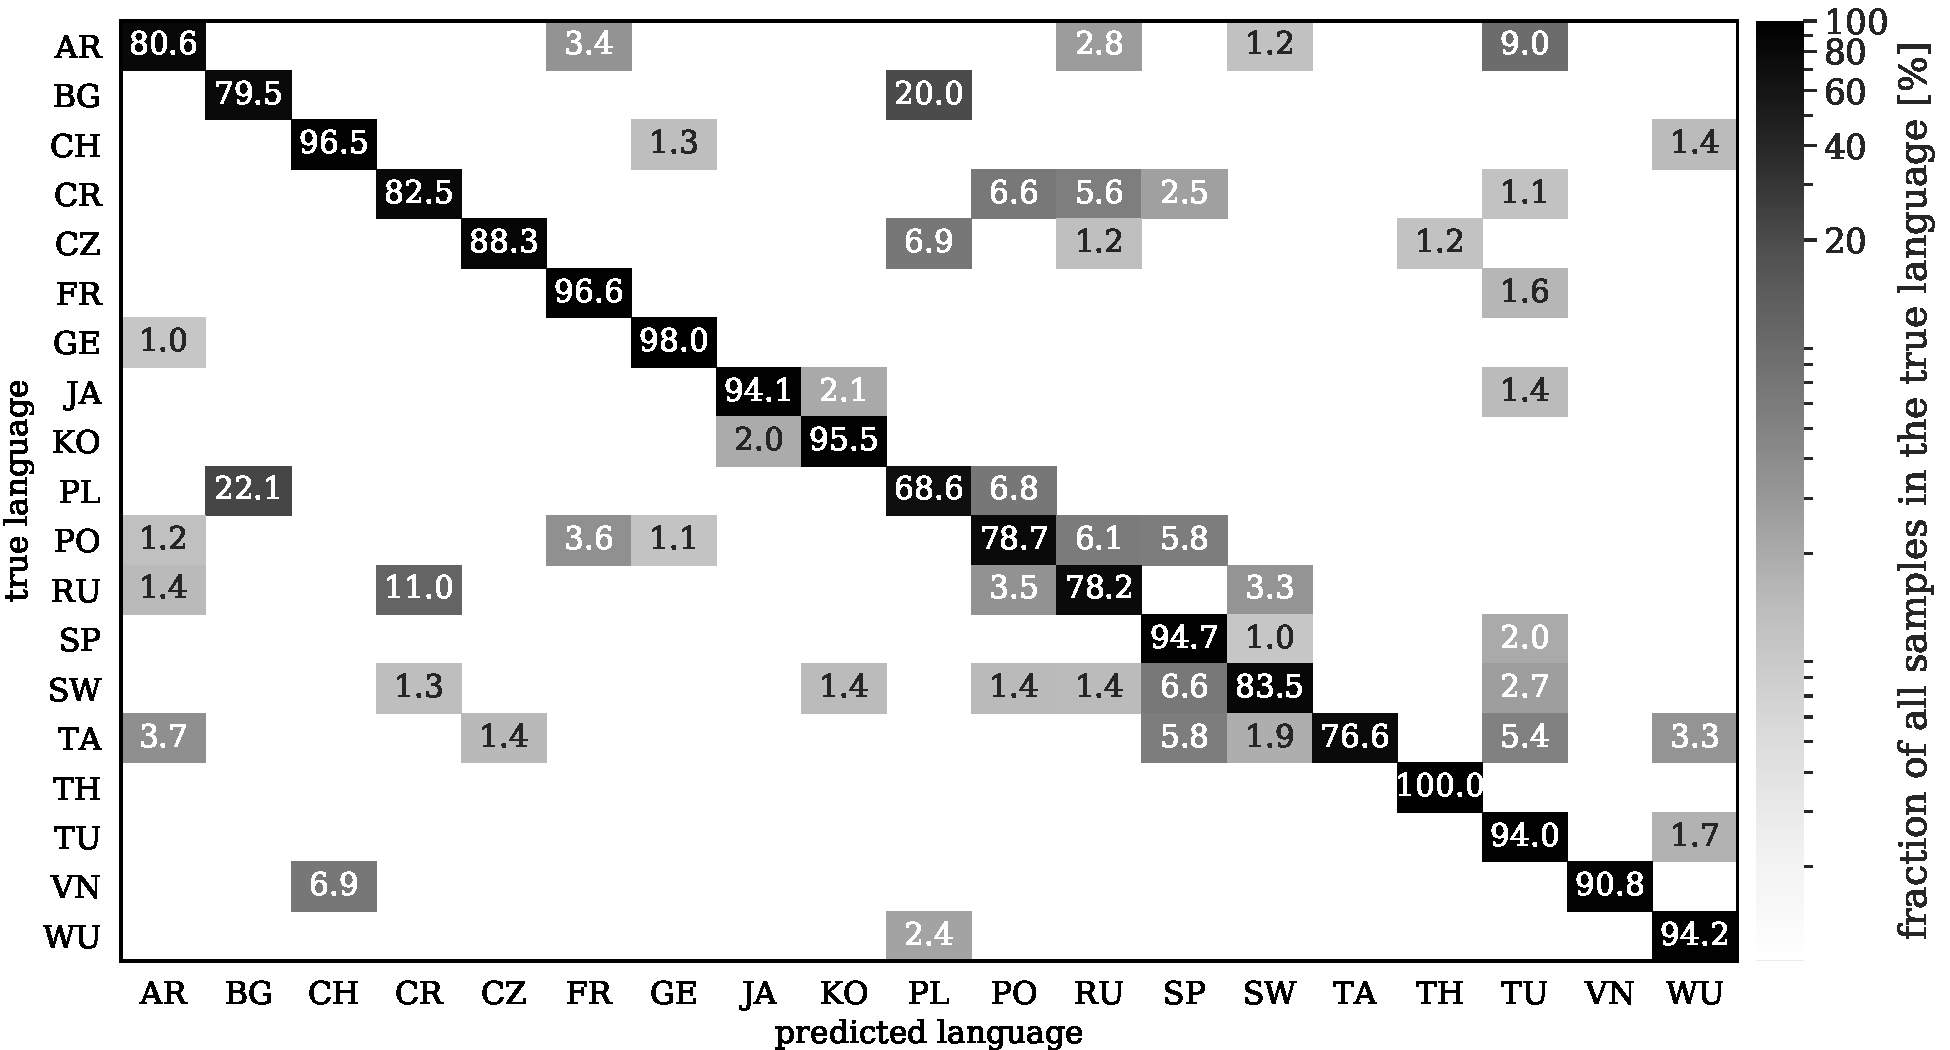
\includegraphics[width=\textwidth]{../img/cfmtrx_pitch_energy.pdf}
      \caption{The confusion matrix for the best prosodic system (energy + pitch combined using early fusion) in the 10s condition. Each cell shows the fraction of all segments labelled as the true language which were classified as the predicted language. Values under 1\% are not shown and logarithmic colour scale is used for better readability.}
      \label{fig:cfmtrx_pitch_energy-10s}
    \end{figure}

    To analyse the prosodic features in more detail, I visualise the confusion matrix for the best-performing prosodic system in the 10s condition (see \autoref{fig:cfmtrx_pitch_energy-10s}). Among the most easily confused language pairs (with the matrix entries above 5\%), most can be explained by their shared language genus\footnote{Genus denotes a language grouping more fine-grained than language families; for instance, the Slavic genus is part of the Indo-European language family.}: pairs of Slavic languages (Polish-Bulgarian, Bulgarian-Polish, Russian-Croatian, Czech-Polish, Croatian-Russian), Chinese languages (Mandarin-Wu), and Romance languages (Portuguese-Spanish). An interesting example is Portuguese being confused with Slavic languages like Polish, Russian or Croatian -- corresponding to the known phenomenon of Portuguese "sounding like" Slavic languages. This can be related to the similar characteristic use of sibilant sounds, vowel reduction (resulting in clusters of consonants) and stress-timed rhythm in Portugal as well as the Slavic languages\footnote{To a curious reader I recommend this video focusing on phonological similarities between Portuguese and Russian/Polish: \url{https://www.youtube.com/watch?v=Pik2R46xobA}}. Still, a good number of confused pairs is difficult to explain phonologically, mainly Arabic-Turkish, Swedish-Spanish, and Tamil being confused for Spanish and Turkish. For these cases, I go back to \autoref{fig:logit-priors} and hypothesise that the reason is the high scaling of priors for Turkish and Spanish (along with other languages such as Croatian, Arabic, and Wu), which can surface in the classifier being biased in favour of these languages.

    \begin{figure}[h!]
      \centering
      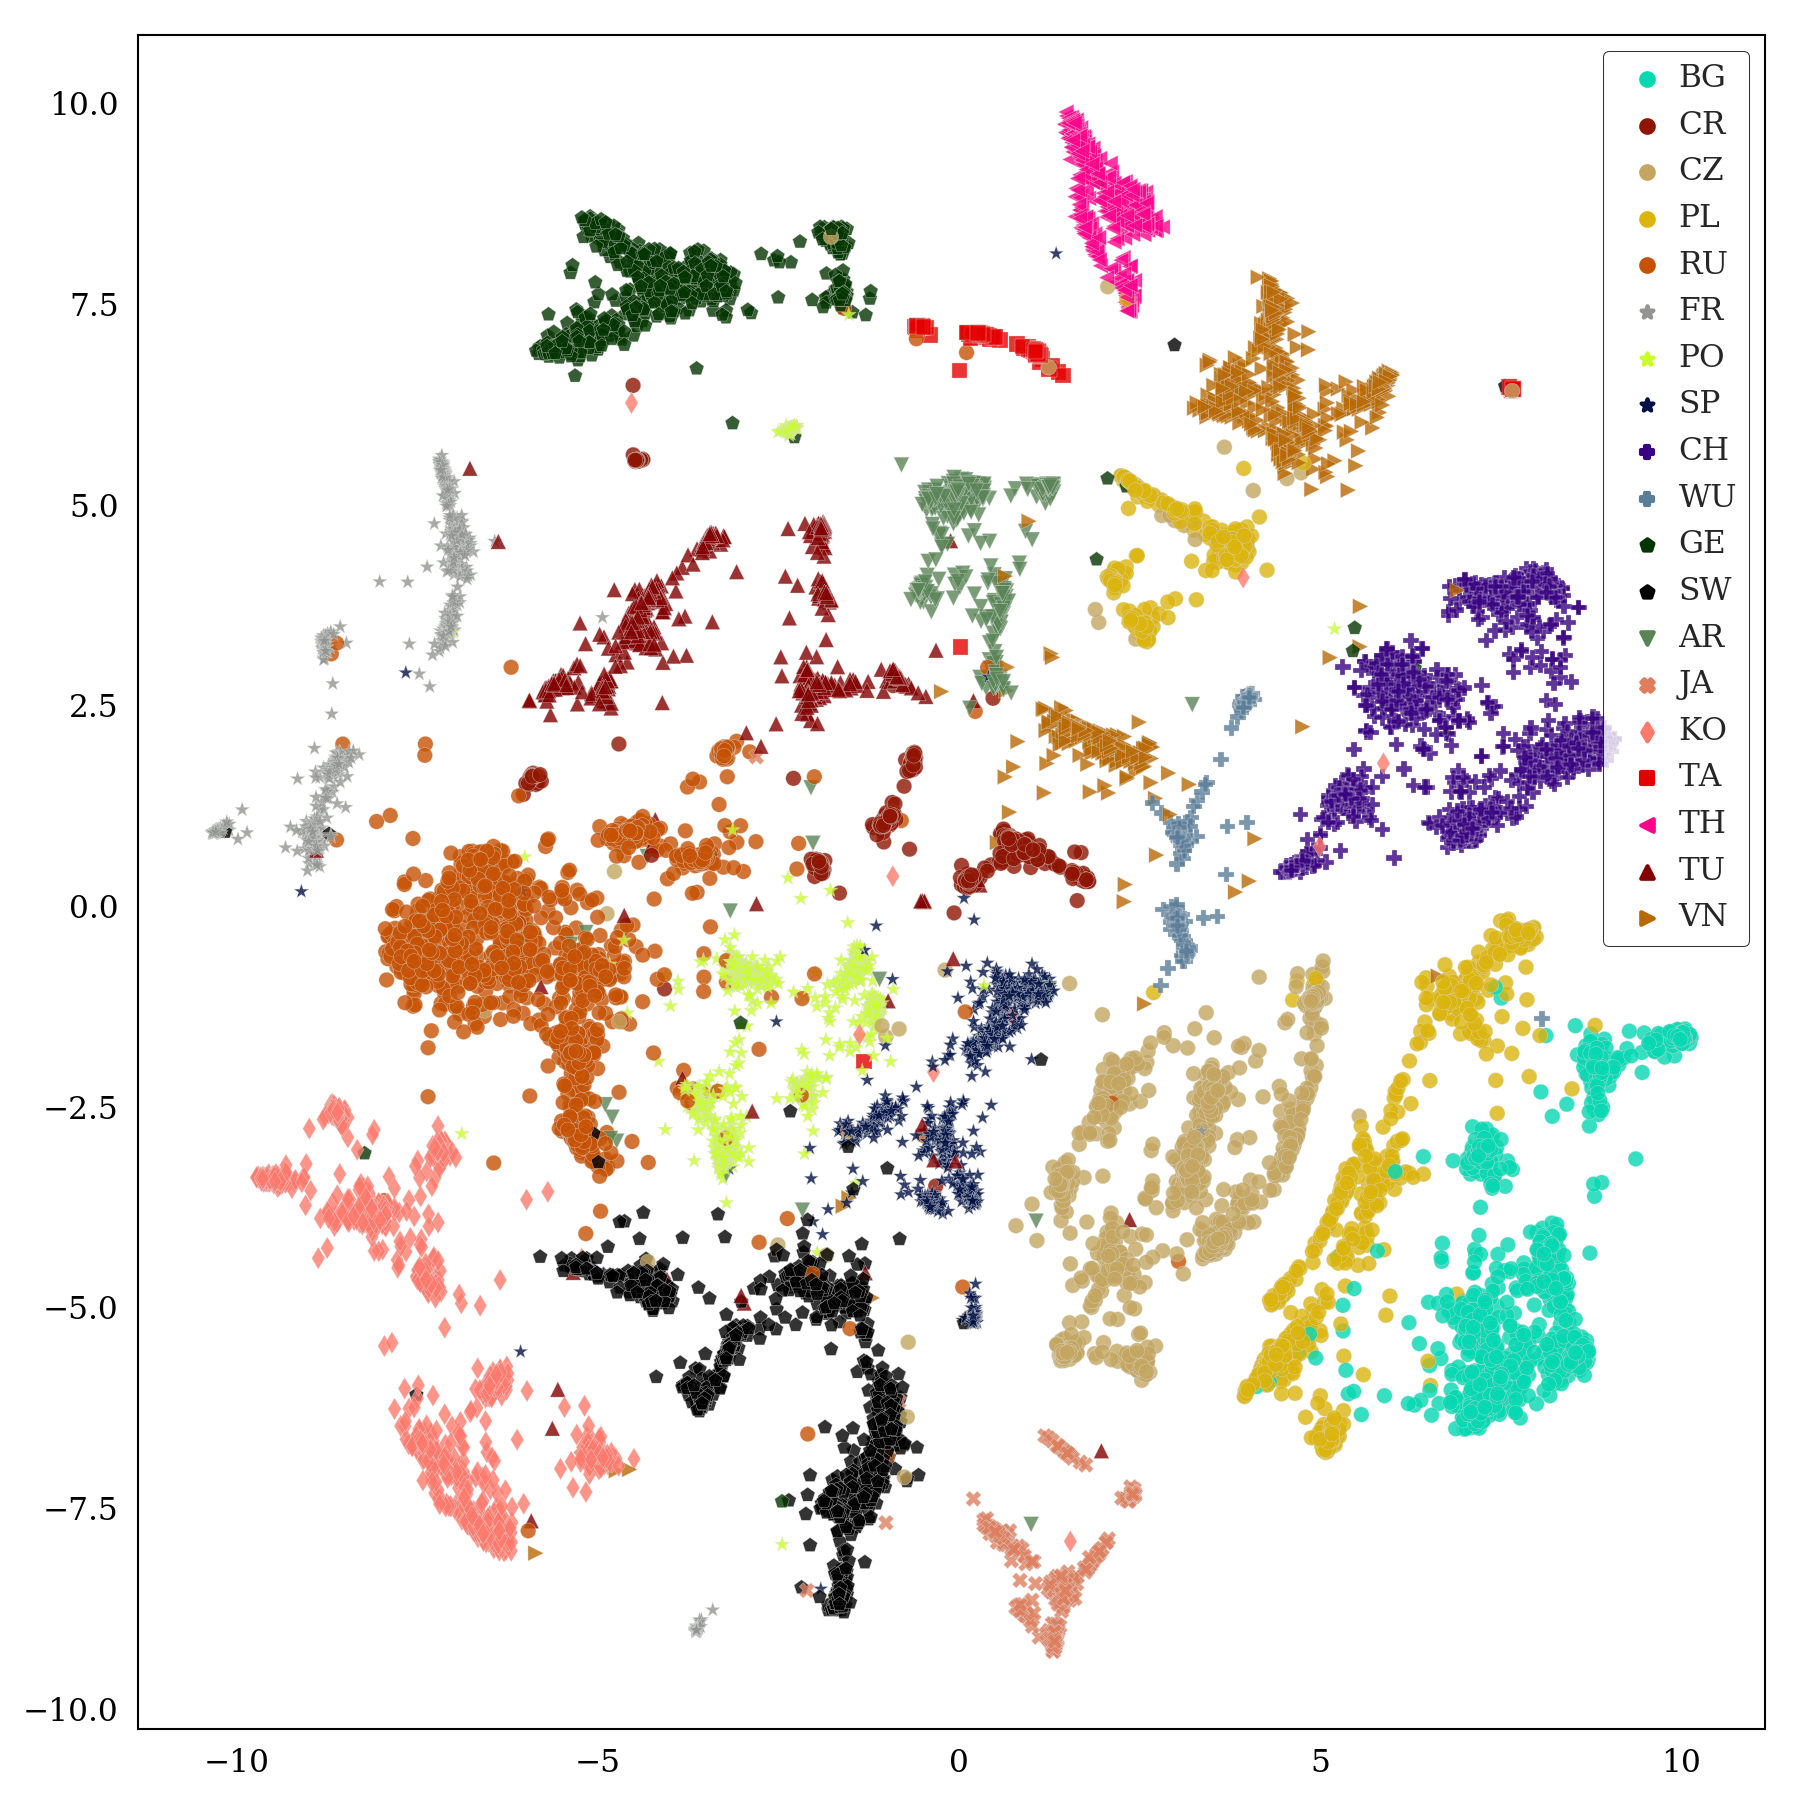
\includegraphics[width=\textwidth]{../img/tsne-pitch_energy.png}
      \caption{Visualisation of the space of the testing set x-vectors extracted from the best prosodic TDNN. Languages from the same genus use the same shape: circle -- Slavic, star -- Romance, cross -- Chinese, pentagon -- Germanic.}
      \label{fig:tsne-pitch_energy}
    \end{figure}
    For added insights into the nature of the prosodic x-vector representation space, I use the t-Distributed Stochastic Neighbour Embedding (t-SNE) technique\footnote{Originally proposed by \citet{Maaten_Hinton_2008}, but I use the implementation from the scikit-learn toolkit: \url{https://scikit-learn.org/stable/modules/generated/sklearn.manifold.TSNE.html}.} to visualise the testing set x-vectors (in the 10s condition) extracted from the best prosodic TDNN, see \autoref{fig:tsne-pitch_energy}. In particular, the way the language clusters are split into visible sub-clusters very strongly correlates with the number of different dominant dialects present in the GlobalPhone data for the given language\footnote{I gathered the dialect information from the speaker metadata files of the GlobalPhone corpus. Note that no dialect details were present for Bulgarian, Wu, Czech, French, German, Polish, Russian, Tamil and Thai}: The Northern and Southern Vietnamese dialects; the Smaalaendska, Goeteborgska and Oelaendska Swedish dialects; the Anatolian and Standard Turkish dialects; the Seoul and Chonnam Korean dialects; the Bosnian, Standard Croatian, and Zagreb Croatian; and the numerous Mandarin and Japanese dialects. This observation suggests that the prosodic features are useful for \textit{dialect identification}. After all, it comes as no surprise: As I mentioned earlier, intonation -- among other prosodic variables -- often characterises the different dialects of a language.

  }

  \section{Combining acoustic and prosodic features}{
    \label{sec:exp-acoustic+prosodic}

    Having shown the individual performances of acoustic and prosodic systems, this experiment finds out whether -- and to what extent -- the acoustic and prosodic information is complementary, i.e. leading to improved performance when combined. For each acoustic feature type, I combined it with (one or both) prosodic features using either early or intermediate fusion. Notice that -- for obvious reasons -- the pipeline does not allow the two prosodic features to be fused at the intermediate (x-vector) level and then combined with an acoustic system at the early level. However, three feature types can be combined all at the feature level (early fusion), or the two prosodic features (combined at any of the two levels) can be combined with an acoustic system at the intermediate level.

    \begin{table}[h!tb]
      \centering
      \begin{sc}
        \footnotesize
        \begin{tabular}{ll|cc|cc}
          &         & \multicolumn{2}{c|}{10s}  & \multicolumn{2}{c}{3s} \\
          \multicolumn{2}{c|}{feature combination} & $C_{primary}$ & accuracy & $C_{primary}$ & accuracy \\
          \hline
          \multirow{3}{*}{\rotatebox[origin=c]{90}{\makecell{MFCC\\ \\+}}}
          & pitch & 0.0693 & 0.941 & 0.153 & 0.871 \\
          & energy & 0.0581 & 0.952 & 0.137 & 0.888 \\
          & pitch + energy & 0.0562 & 0.954 & 0.136 & 0.889 \\
          \hline
          \multirow{3}{*}{\rotatebox[origin=c]{90}{\makecell{MFCC+\\$\Delta$+$\Delta\Delta$\\+}}}
          & pitch & 0.0577 & 0.950 & 0.134 & 0.886 \\
          & energy & 0.0523 & 0.957 & 0.129 & 0.895 \\
          & pitch + energy & 0.0544 & 0.956 & 0.139 & 0.888 \\
          \hline
          \multirow{3}{*}{\rotatebox[origin=c]{90}{\makecell{SDC\\ \\+}}}
          & pitch & 0.0559 & 0.952 & 0.159 & 0.867 \\
          & energy & \textbf{0.0401} & 0.967 & \textbf{0.128} & 0.896 \\
          & pitch + energy & 0.0484 & 0.960 & 0.137 & 0.888 \\
        \end{tabular}
      \end{sc}
      \caption{Combining acoustic and prosodic features (early fusion used in all instances).}
      \label{tab:results-combined-early}
    \end{table}

    \begin{table}[h!tb]
      \centering
      \begin{sc}
        \footnotesize
        \begin{tabular}{ll|cc|cc}
          &         & \multicolumn{2}{c|}{10s}  & \multicolumn{2}{c}{3s} \\
          \multicolumn{2}{c|}{feature combination} & $C_{primary}$ & accuracy & $C_{primary}$ & accuracy \\
          \hline
          \multirow{4}{*}{\rotatebox[origin=c]{90}{\makecell{MFCC\\ \\+}}}
          & pitch & 0.0624 & 0.950 & 0.138 & 0.886 \\
          & energy & 0.0556 & 0.956 & 0.149 & 0.878 \\
          & pitch + energy (early) & 0.0382 & 0.968 & 0.107 & 0.910 \\
          & pitch + energy (intermediate) & 0.0501 & 0.958 & 0.132 & 0.890 \\
          \hline
          \multirow{4}{*}{\rotatebox[origin=c]{90}{\makecell{MFCC+\\$\Delta$+$\Delta\Delta$\\+}}}
          & pitch & 0.0467 & 0.961 & 0.120 & 0.900 \\
          & energy & 0.0508 & 0.960 & 0.140 & 0.886 \\
          & pitch + energy (early) & \textbf{0.0343} & 0.971 & \textbf{0.0993} & 0.918 \\
          & pitch + energy (intermediate) & 0.0511 & 0.959 & 0.129 & 0.895 \\
          \hline
          \multirow{4}{*}{\rotatebox[origin=c]{90}{\makecell{SDC\\ \\+}}}
          & pitch & 0.0622 & 0.949 & 0.142 & 0.881 \\
          & energy & 0.0674 & 0.947 & 0.167 & 0.864 \\
          & pitch + energy (early) & 0.0376 & 0.968 & 0.114 & 0.906 \\
          & pitch + energy (intermediate) & 0.0545 & 0.954 & 0.139 & 0.883 \\

        \end{tabular}
      \end{sc}
      \caption{Combining acoustic and prosodic systems using intermediate fusion (the combinations of 2 prosodic features used early or intermediate fusion).}
      \label{tab:results-combined-intermediate}
    \end{table}

    \autoref{tab:results-combined-early} shows the results for systems in which an acoustic system and a prosodic one were combined using early fusion, while \autoref{tab:results-combined-intermediate} refers to the systems in which acoustic and prosodic information was combined at the intermediate (x-vector) level. Regardless of the fusion type, combining acoustic and prosodic information clearly improves the performance. The best system uses \textit{both} prosodic features combined as a pair at the feature level (early fusion), which is not surprising, having compared the prosody-only systems in \autoref{sec:exp-prosodic}.
    % prosody and acoustic representations best combined at x-vector level: it may be that they are difficult for the TDNN to combine since they bear so different information
    For combining acoustic information with prosody, however, intermediate fusion improves on early fusion by 14\% and 22\% in the 10s and 3s conditions, respectively.
    While this phenomenon needs to be investigated further, I hypothesise that the TDNN was not able to combine acoustic and prosodic features well because of their different nature: Besides representing very different properties of speech, the features also differ in their level of abstraction. While the pitch and energy features are very close to the raw values capturing the corresponding prosodic contours, MFCCs (and derived features) have gone through many sophisticated transforms in order to be low-dimensional and decorrelated. To investigate this hypothesis, an acoustic feature much closer to the original power spectrum could be used, such as the Mel filter bank features (in essence, these are an intermediate stage features in the MFCC pipeline, see \autoref{fig:mfcc}).
    
    % huge improvement compared to acoustic systems
    Most importantly, the best acoustic system is largely outperformed by the best combined system: the relative improvement in terms of $C_{primary}$ is 37\% and 28\% for the 10s and 3s conditions, respectively. This is more than twice the improvement reported by \citet{Martinez_et_al_2012} after fusing a prosodic i-vector system modelling pitch, energy and duration with a then state-of-the-art acoustic i-vector system (they report the relative improvement of 15.24\% and 10.93\% for the 10s and 3s conditions).
    % naturally, architectures like x-vectors provide good opportunities for prosody, since they can aggregate temporal contexts (no longer the need for hacks like Legendre polynomials, duration numbers or other implicit time capturing)
    I attribute this big difference in improvements primarily to the better suitability and power of a temporal context aggregating model like TDNN. Remember that the i-vector system applies the bag-of-frames approach, which has to be compensated for by more sophisticated feature engineering: In this case, \citeauthor{Martinez_et_al_2012} for each frame approximated the local pitch and energy contours by Legendre polynomials, whose coefficients served as the feature values for the given frame.

    I hypothesise that another possible reason why prosody improved performance much more in my case is the channel difference between the NIST LRE 2009 dataset\footnote{\url{https://catalog.ldc.upenn.edu/LDC2014S06}} used by \citeauthor{Martinez_et_al_2012} and the GlobalPhone corpus I used. The lower sampling rate (8kHz) of the LRE data should not make a big difference -- the usual pitch range is $\leq$500Hz. The varied and noisy recording environment (the LRE 2009 data consists of telephone speech and radio broadcast conversations), on the other hand, can in my opinion pose a challenge for extracting good-quality prosodic information, and I plan to explore this phenomenon in my future work.

    My last point relates to the decision to not use energy as part of the MFCC features (in line with the work of \citet{Snyder_et_al_2018}). One could object that energy is often used with MFCCs and excluding it makes the prosodic systems perform worse. My results confirm this: When comparing the MFCC results from \autoref{tab:results-acoustic} and the corresponding results of MFCCs with energy added at feature level (\autoref{tab:results-combined-early}), the energy brings a relative improvement of 12\% (7.4\% in the 3s condition). This improvement suggests significant usefulness of energy on top of the information captured by the 0\textsuperscript{th} cepstral coefficient. I believe, however, that my decision to use MFCC features without energy was justified as I wanted to analyse how much useful information the different prosodic features capture when compared to acoustic features.
  }
}

\chapter{Overall discussion and conclusions}{
  \label{chap:discussion-and-conclusions}

  In this chapter, I provide an overall discussion of my results and findings in the context of past research, elaborate more on the limitations of my work, and draw conclusions.

  \begin{figure}[h!]
    \centering
    \begin{minipage}{0.49\textwidth}
      \centering
      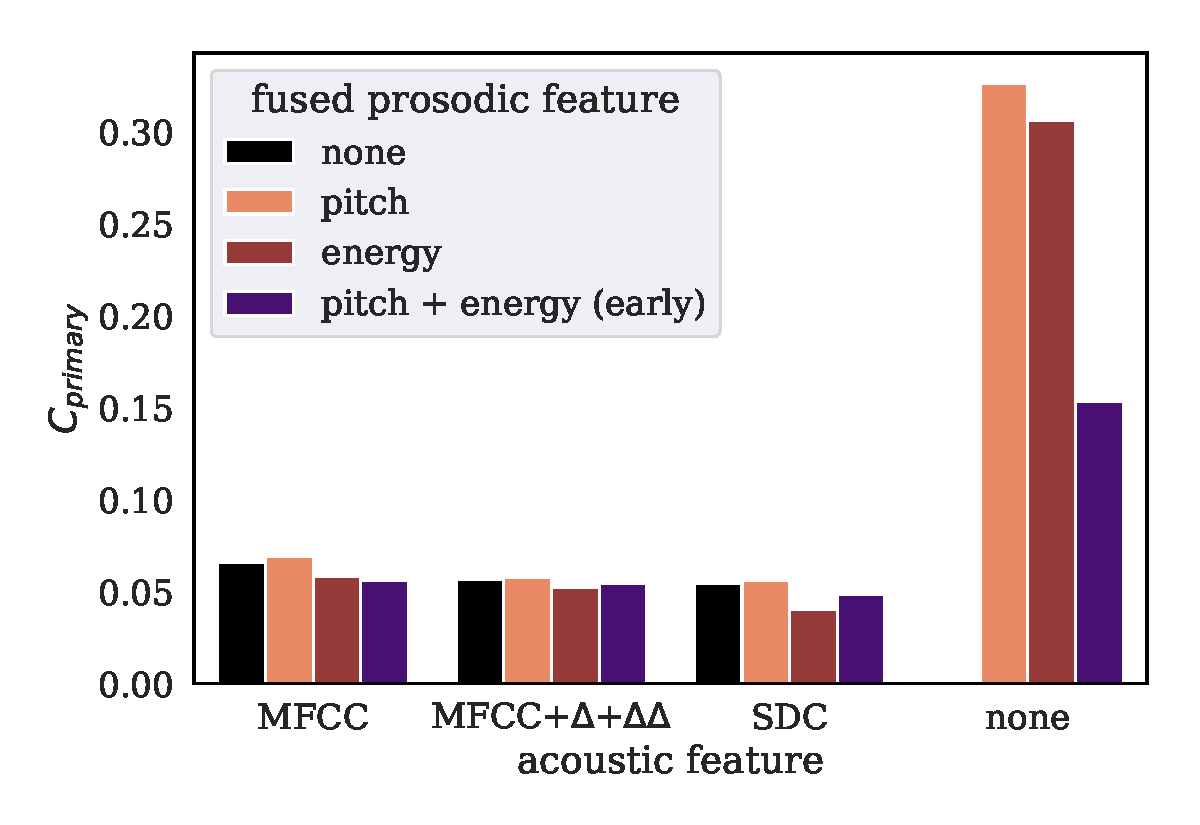
\includegraphics[width=\textwidth]{../img/summary-early-10s.pdf}
      \subcaption{Early fusion, 10s condition.}
      \label{fig:summary-early-10s}
    \end{minipage}
    \begin{minipage}{0.49\textwidth}
      \centering
      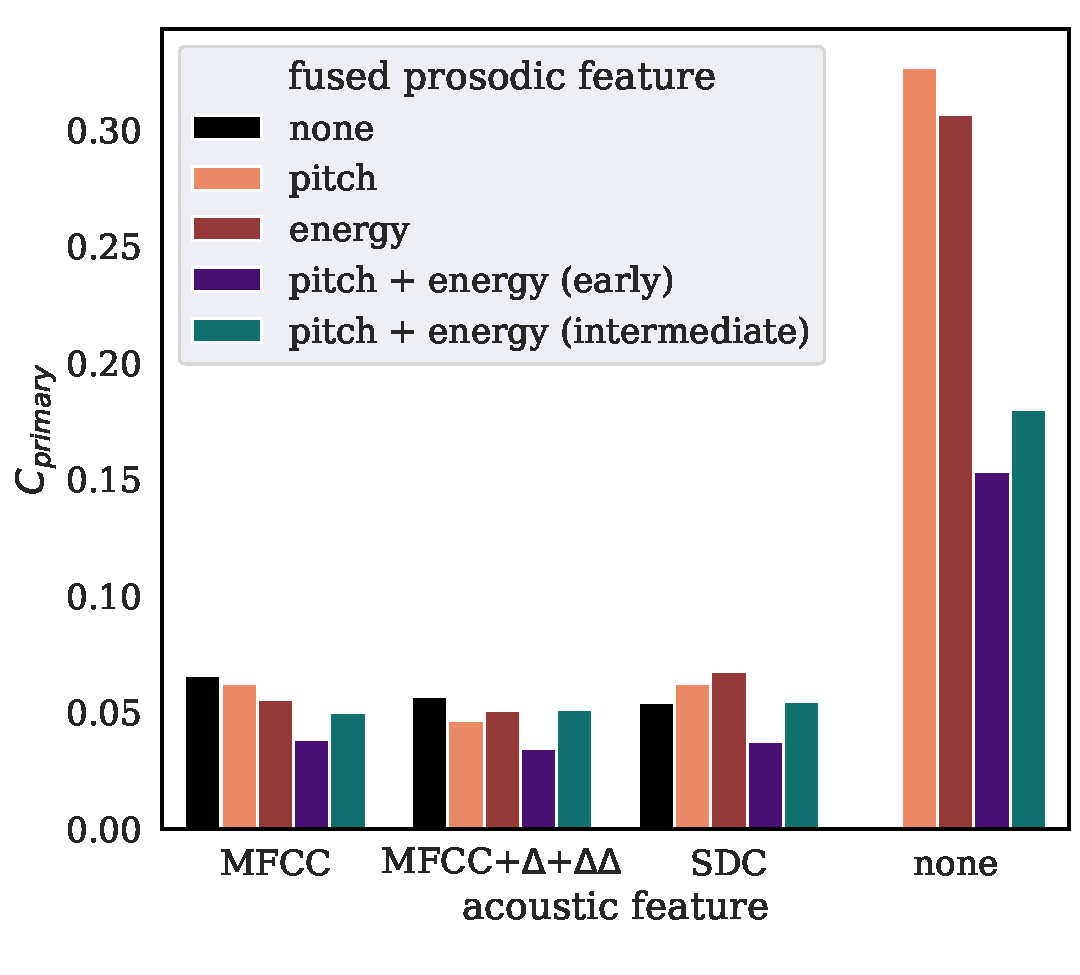
\includegraphics[width=\textwidth]{../img/summary-intermediate-10s.pdf}
      \subcaption{Intermediate fusion, 10s condition.}
      \label{fig:summary-intermediate-10s}
    \end{minipage}
    \begin{minipage}{0.49\textwidth}
      \centering
      \vspace*{1.5em}      
      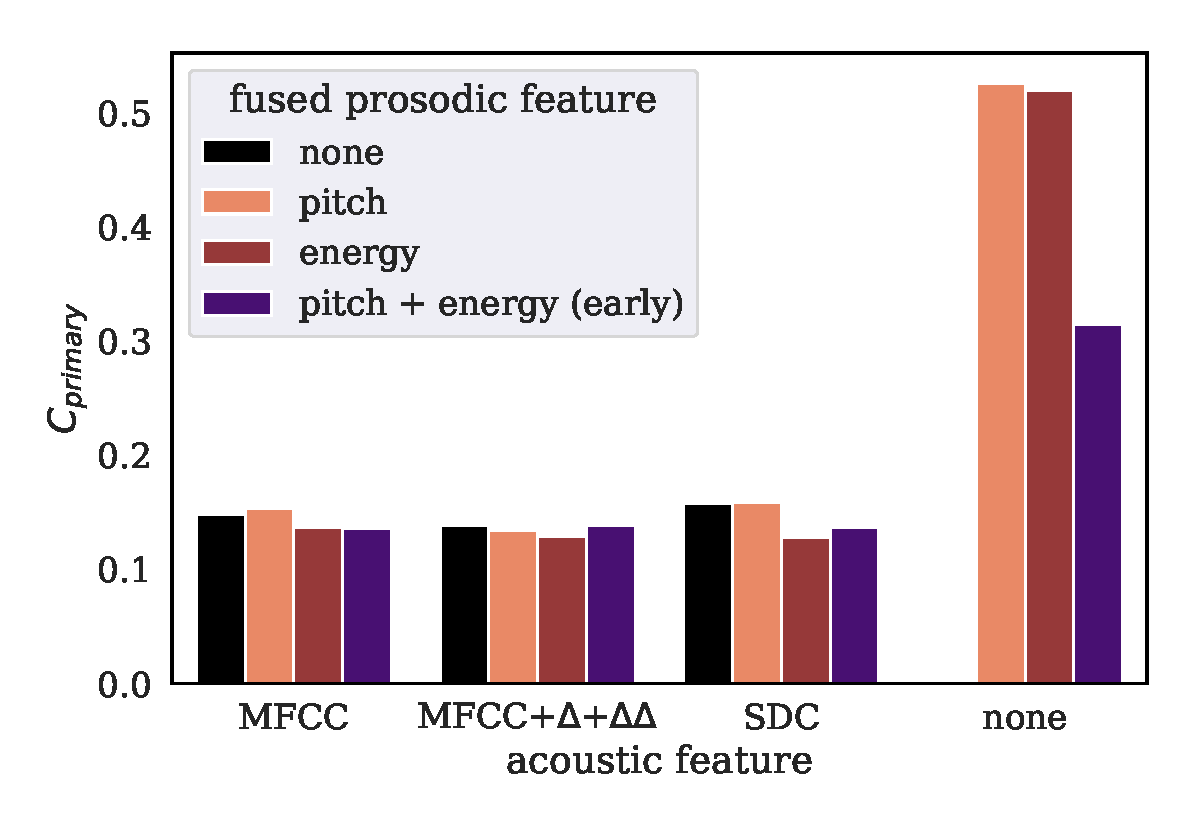
\includegraphics[width=\textwidth]{../img/summary-early-3s.pdf}
      \subcaption{Early fusion, 3s condition.}
      \label{fig:summary-early-3s}
    \end{minipage}
    \begin{minipage}{0.49\textwidth}
      \centering
      \vspace*{1.5em} 
      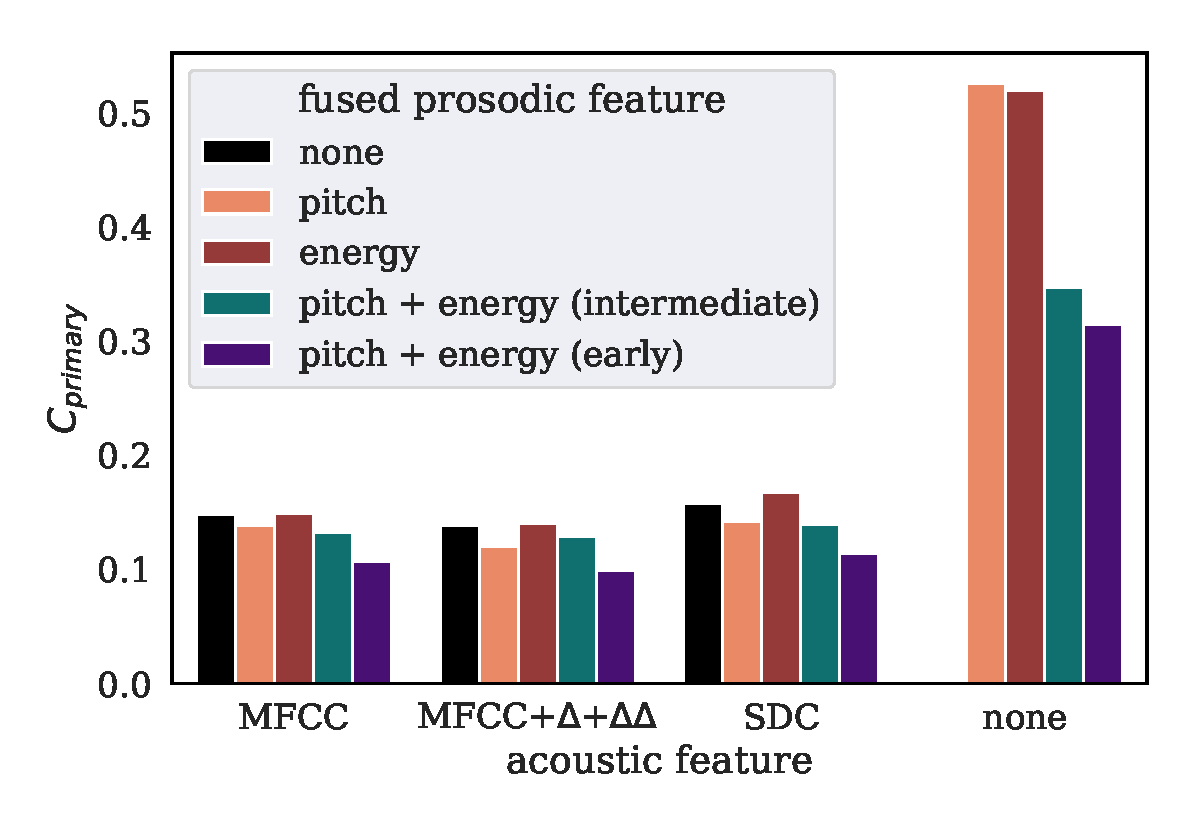
\includegraphics[width=\textwidth]{../img/summary-intermediate-3s.pdf}
      \subcaption{Intermediate fusion, 3s condition.}
      \label{fig:summary-intermediate-3s}
    \end{minipage}
    \caption{Final comparison of all acoustic+prosodic combinations in the 10s (top) and 3s (bottom) condition, where the acoustic and prosodic information is combined at the feature (early) level (left) and at the x-vector (intermediate) level (right).}
    \label{fig:summary-barplots}
  \end{figure}


  %%% comment on the overall comparisons between combinations of features
  pitch+energy (early) by far the biggest improvement (choice of acoustic feature doesn't matter too much strictly speaking). this is very good because prosodic tdnn can be trained spearately, the clssifier then retrained and here we go!
  relative improvements smaller on short segments; usual thing observed in Snyder and Martinez as well...
  tdnn unable to process pitch with acoustic info well (same or slightly worse performance in early fusion).
  interestingly, sdc tdnn struggling with pitch and energy in intermediate fusion! (when isolated)


  %%% comment on language-specific performance of the best model
  % languages with information on sex: AR, BG, WU, CR, CZ, FR, GE, JA, KO, CH, PL (only 1/3), PO, RU, SP, SW, TH, TU, VN. without: TA, PL (partial),
  confusing pairs:
  PO-SP
  CR-PO
  PL-BG
  CZ-PL
  WU-CH
  PO-RU
  SW-SP
  spanish preferred by the classifier (unfair!). but then simply romance, slavic and chinese pairs confused (good), and portuguese with slavic languages (fair, discussed earlier)
  
  F1
  best languages: CH, FR, GE, TA, TH
  worst languages: PO, CR, SP, PL
  cannot be easily attributed to sex imbalance
  
  let's plot eval/test imbalance to see if adjusting the prior was unfair for some languages
  - most heavy adjustments were made for: AR, CR, SP, TU, WU, vs JA, VN
  - most of these languages have eval and test distribution similar, except WU and VN, but these were recognised fine! (95.7 and 99.5)
  remarkable: just 1h of training data and 0.8h of enrollment was enough for the TDNN and classifier and we have 0.992 F1!

  \begin{figure}[h!]
    \centering
    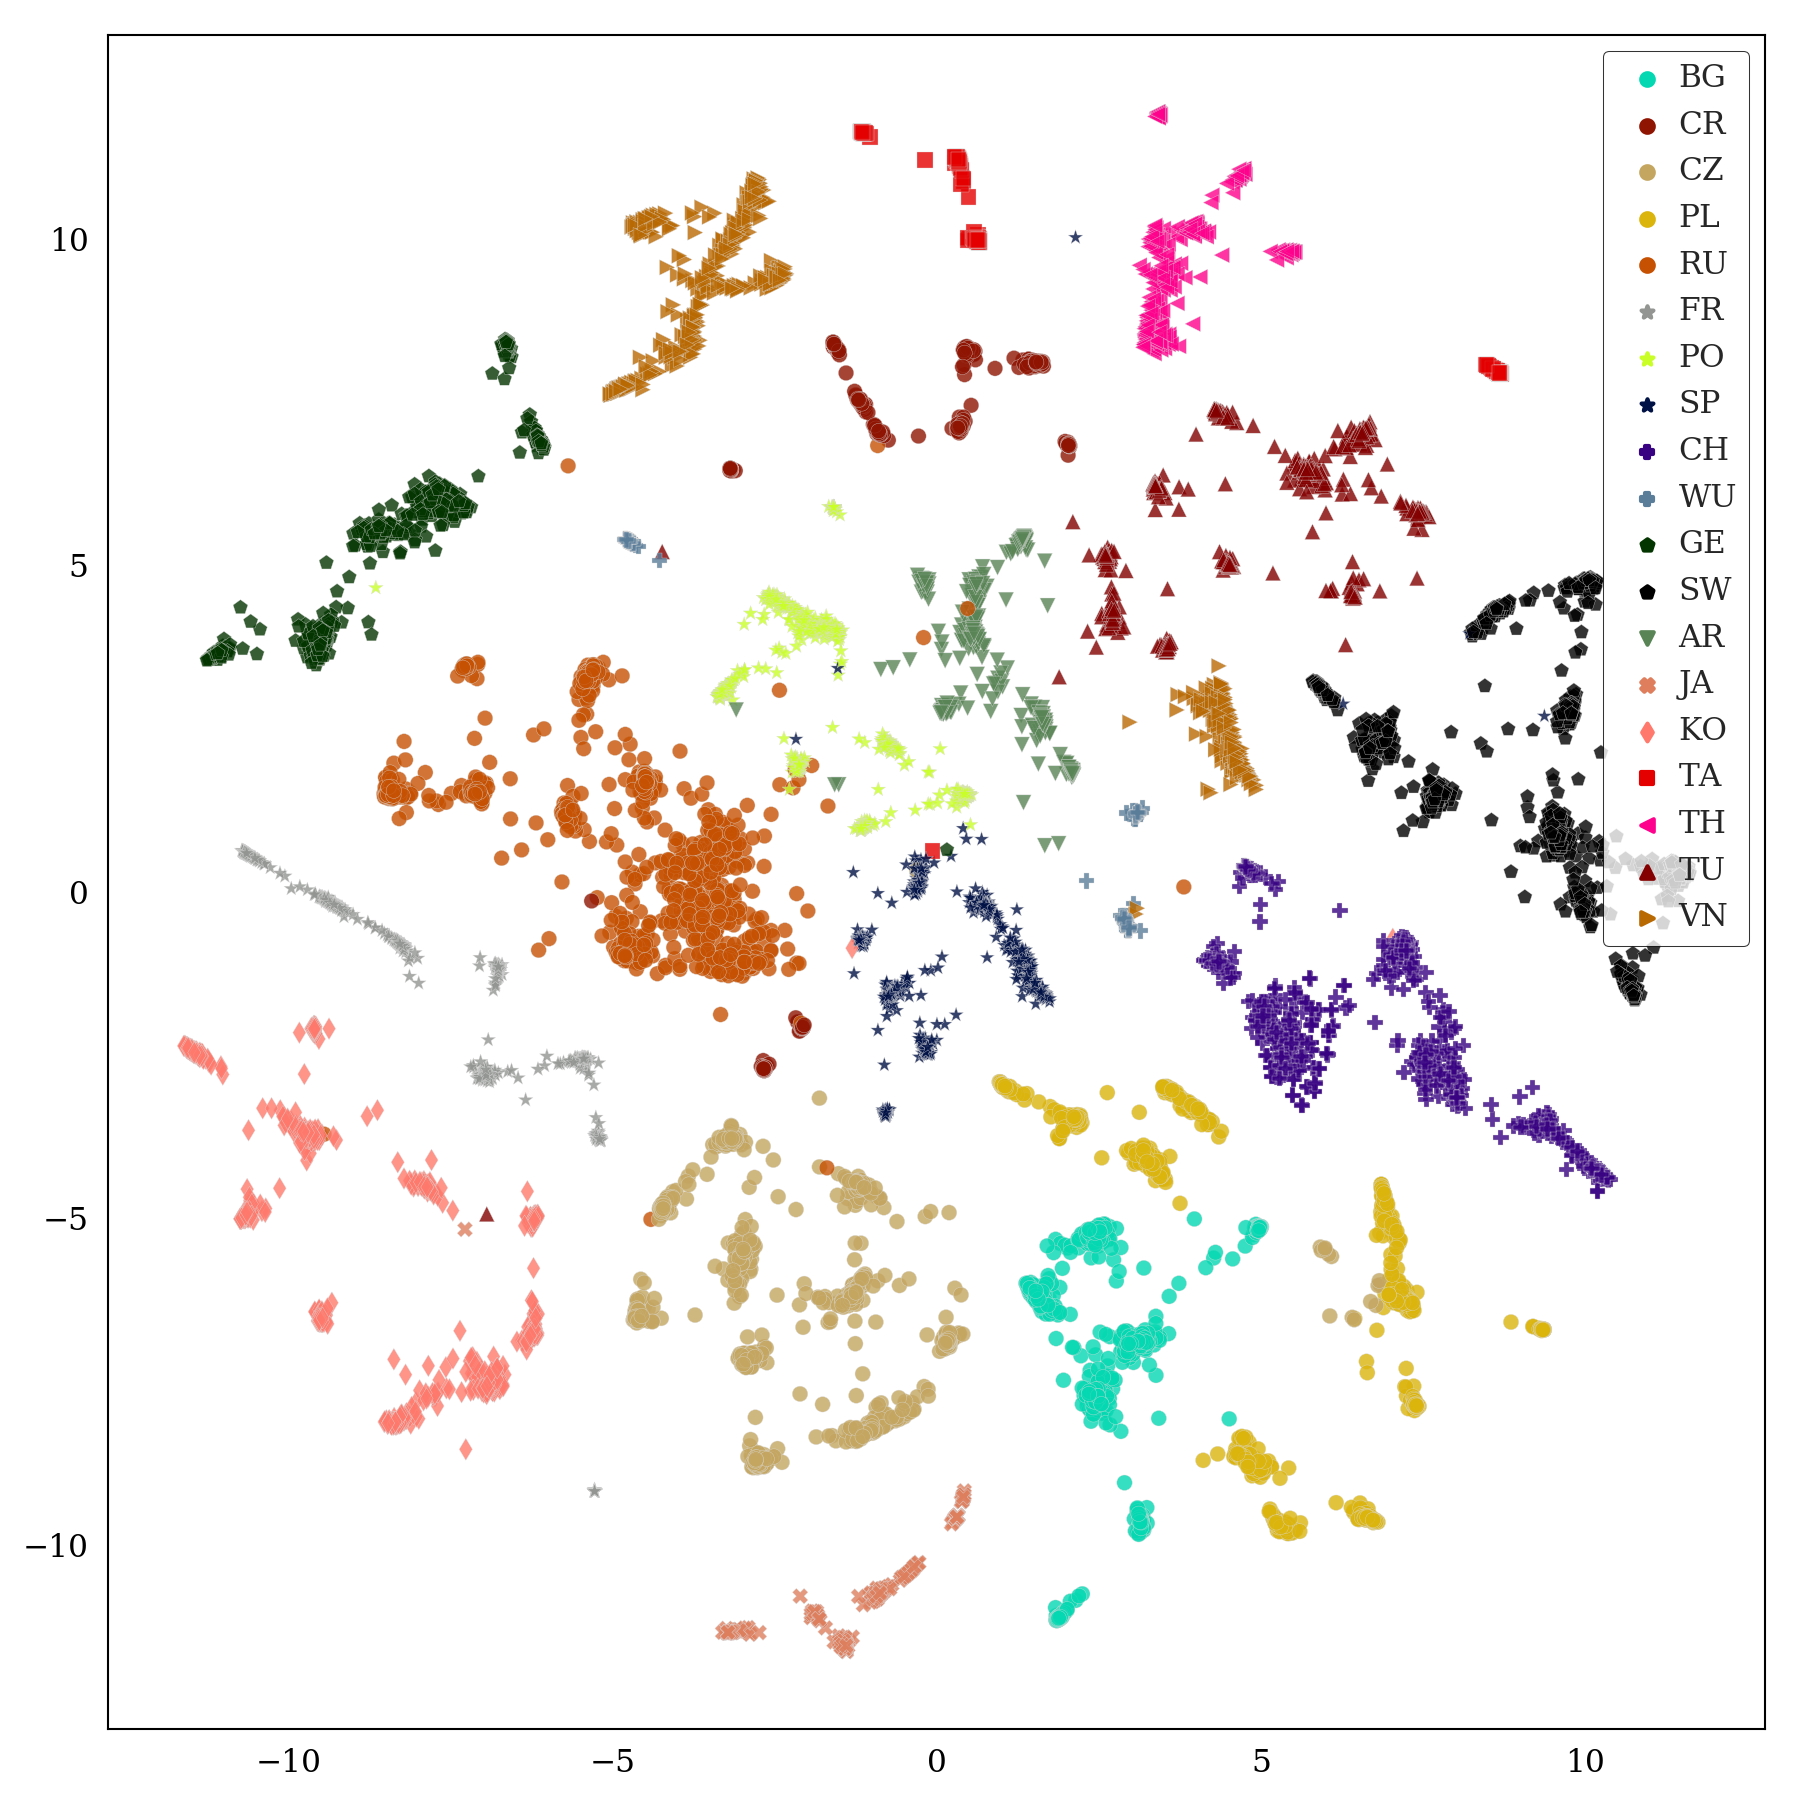
\includegraphics[width=\textwidth]{../img/tsne-mfcc_deltas_pitch_energy.png}
    \caption{Early fusion, 10s condition.}
    \label{fig:summary-early-10s}
  \end{figure}

  \begin{figure}[h!]
    \centering
    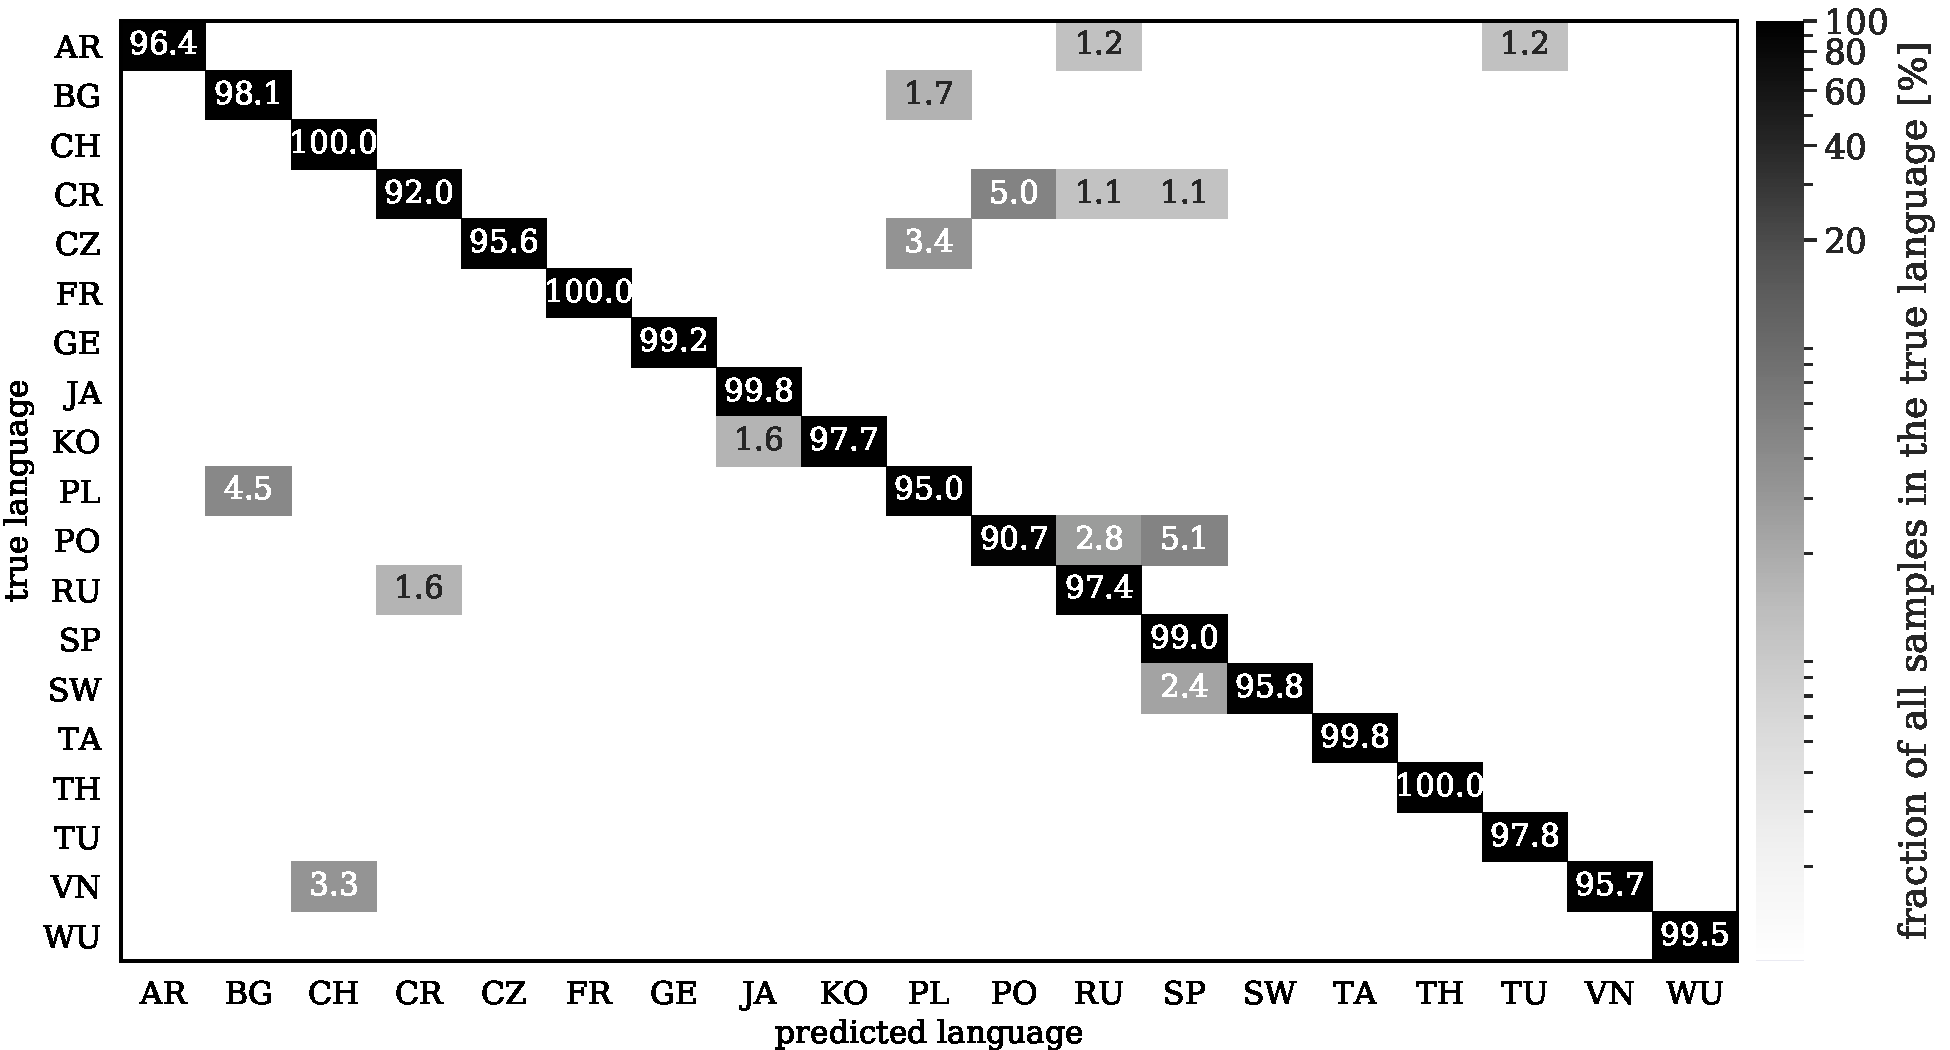
\includegraphics[width=\textwidth]{../img/cfmtrx_fusion_mfcc_deltas+pitch_energy.pdf}
    \caption{Early fusion, 10s condition.}
    \label{fig:summary-early-10s}
  \end{figure}


  %%% comment on language-specific trends w.r.t prosody
  where does prosody struggle the most? difference between best and prosodic only
  where is prosody most helpful? difference between best and acoustic only


  %%% conclusions
  prosody helps a lot (as much as 37 and 28\%)
  pitch and energy are hugely complementary and should be used together. duration is captured for free when using x-vectors :-)
  prosody better modelled with x-vectors than with i-vectors, and the features are simpler
  energy has a lot to offer on top of C0
  Martinez (2013) mention that in "Continuous Prosodic Features and Formant Modeling with Joint Factor Analysis for Speaker Verication" formants on top of acoustic system don't help (haha, surprise), but in their work they do help: with added formants (on top of prosody), the improvement is 17.79\% (14.92\%) compared to then SOTA acoustic i-vector system without prosody or formants
  I ignore BNFs (as used by Snyder and some others). In essence, they're computed from acoustic features. I just wanna know how much the prosodic information can help when combined with acoustic information.
}

\chapter{Future work}{
  \label{chap:future-work}

  \section{Possible directions}{
    Everything that is sensible but unlikely in Year 5.

    compute VAD correctly

    explore segment boundary effects (but note that uniform segmentation shown to work well: Steve mentioned speaker diarization, I have \citet{Martinez_et_al_2013} that show the same...)

    try late (score) fusion

    try bottleneck features instead of acoustic ones and see how much prosody can help

    use more noisy data or narrowband to see how well the energy and Kaldi pitch can be extracted there
  }

  \section{Plan for Part 2 of the MInf project}{

  }
}

\chapter{Conclusions}{
  \label{chap:conclusions}
  ...
}

\bibliographystyle{apalike}
\bibliography{s1513472-minf1}

\appendix

\chapter{Partitioning of the dataset}{
  \begin{sc}
    \centering
    \footnotesize
    \begin{longtable}{p{0.5cm}|p{0.8cm}|p{3.9cm}|p{3.5cm}|p{3.5cm}}
      & train. & enrollment & evaluation & testing \\
      \hline
      AR & 57 & 017, 023, 056, 104, 105, 114, 135 & 014, 030, 047, 067, 109, 115, 137 & 011, 012, 027, 050, 051, 055, 066 \\
      \hline
      BG & 56 & 042, 048, 056, 065, 088, 104, 107 & 051, 055, 058, 084, 090, 100, 106 & 040, 059, 063, 068, 095, 109, 110 \\
      \hline
      CH & 98 & 004, 005, 012, 034, 035, 036, 045, 048, 052, 053, 057, 120, 126 & 028, 029, 030, 031, 032, 039, 040, 041, 042, 043, 044 & 080, 081, 082, 083, 084, 085, 086, 087, 088, 089 \\
      \hline
      CR & 63 & 001, 010, 018, 026, 029, 032, 074, 092, 093 & 033, 034, 035, 036, 046, 048, 051, 053, 054, 057 & 037, 038, 039, 040, 041, 042, 043, 044, 045, 047 \\
      \hline
      CZ & 72 & 005, 009, 031, 033, 034, 036, 053, 061, 071, 072 & 083, 085, 087, 089, 091, 093, 095, 097, 099, 101 & 084, 086, 088, 090, 092, 094, 096, 098, 100, 102 \\
      \hline
      FR & 74 & 009, 028, 030, 031, 033, 052, 064, 065, 070, 076 & 082, 083, 084, 085, 086, 087, 088, 089 & 091, 092, 093, 094, 095, 096, 097, 098 \\
      \hline
      GE & 58 & 015, 017, 046, 056, 058, 065, 074 & 001, 002, 003, 004, 008, 010 & 018, 020, 021, 026, 029, 073 \\
      \hline
      JA & 119 & 002, 021, 037, 048, 051, 053, 057, 064, 086, 201, 202, 206, 209, 221 & 009, 031, 046, 081, 091 & 006, 025, 045, 047, 088, 101 \\
      \hline
      KO & 70 & 018, 030, 043, 044, 057, 065, 074, 078, 079, 090 & 006, 012, 025, 040, 045, 061, 084, 086, 091, 098 & 019, 029, 032, 042, 051, 064, 069, 080, 082, 088 \\
      \hline
      PL & 70 & 008, 018, 032, 076, 083, 085, 088, 096, 099 & 005, 011, 012, 030, 040, 041, 046, 063, 090, 097 & 001, 004, 009, 023, 031, 033, 043, 044, 050, 098 \\
      \hline
      PO & 75 & 070, 071, 106, 109, 117, 120, 128, 146, 148, 150 & 064, 072, 102, 103, 104, 132, 133, 134 & 135, 137, 138, 139, 142, 143, 312 \\
      \hline
      RU & 84 & 017, 023, 035, 041, 088, 101, 114, 115, 119, 121, 123 & 005, 033, 042, 065, 078, 097, 103, 106, 110, 122 & 002, 027, 036, 063, 069, 092, 102, 104, 109, 112 \\
      \hline
      SP & 72 & 037, 041, 048, 059, 060, 064, 074, 083, 098, 099 & 001, 002, 003, 004, 005, 006, 007, 008, 009, 010 & 011, 012, 013, 014, 015, 016, 017, 018 \\
      \hline
      SW & 70 & 001, 013, 023, 070, 072, 077, 078, 080, 084 & 045, 046, 047, 048, 049, 066, 067, 068, 069 & 040, 041, 042, 043, 044, 060, 061, 062, 063, 064 \\
      \hline
      TA & 35 & 022, 028, 038, 047 & 003, 030, 035, 039 & 001, 005, 033, 037 \\
      \hline
      TH & 73 & 001, 005, 027, 031, 041, 065, 067, 077, 083 & 023, 025, 028, 037, 045, 061, 073, 085 & 101, 102, 103, 104, 105, 106, 107, 108 \\
      \hline
      TU & 69 & 010, 017, 044, 048, 049, 051, 064, 091, 093, 096 & 001, 002, 003, 005, 006, 008, 013, 014, 015, 016, 019 & 025, 030, 031, 032, 037, 039, 041, 046, 056, 063 \\
      \hline
      VN & 103 & 012, 029, 031, 036, 043, 050, 053, 070, 077, 118, 119, 128 & 200, 201, 202, 203, 204, 205, 206, 207, 208 & 102, 103, 106, 110, 113 \\
      \hline
      WU & 6 & 008, 011, 013, 015 & 002, 004, 006, 017 & 001, 003, 005, 009 \\
      \hline
      \multicolumn{3}{l}{} \\[-7pt]
      \caption{The partitioning of each language's speakers into the 4 partitions. For enrollment, evaluation and testing sets, speaker IDs are shown. For the training set, the rest of the speakers was used and only the number of speakers is shown.}
      \label{tab:partitioning}
    \end{longtable}
  \end{sc}
}

\end{document}
